\documentclass[letterpaper,twoside,onecolumn,openright,final]{memoir}
%    vs.       others...   oneside twocolumn openleft  draft showtrims
%                          twoside onecolumn openany   ms
%                                            openright final 
\input lumos_common
\begin{document}
\newcommand\z[1]{{\ttfamily #1}}
\newcommand{\colorbitbox}[3]{%
  \rlap{\bitbox{#2}{\color{#1}\rule{\width}{\height}}}%
  \bitbox{#2}{#3}}
\newenvironment{BF}{\begin{center}\begin{bytefield}{8}\bitheader{0-7}\\}{\end{bytefield}\end{center}}
\definecolor{lightgray}{gray}{0.8}
\frontmatter
  \def\lightxbase{0}
  \def\light#1#2{%
    % \light{A/G/Y/R/G2/Y2/R2}{on/off/}   at \y
    % A  G  Y  R            -- both 48 AND 24
    % A1 G1 Y1 R1 G2 Y2 R2  -- 48 only
    % A0 G0 Y0 R0           -- 24 only
    \ifthenelse{\equal{#1}{A}}{\def\lightx{0}\def\lightc{yellow}\def\lighty{.3}\def\lightxx{1.8}\def\lightyy{.45}}{%
      \ifthenelse{\equal{#1}{G}}{\def\lightx{.3}\def\lightc{green}\def\lighty{.3}\def\lightxx{1.5}\def\lightyy{.3}}{%
        \ifthenelse{\equal{#1}{Y}}{\def\lightx{.6}\def\lightc{yellow}\def\lighty{.3}\def\lightxx{1.8}\def\lightyy{.15}}{%
          \ifthenelse{\equal{#1}{R}}{\def\lightx{.9}\def\lightc{red}\def\lighty{.3}\def\lightxx{1.5}\def\lightyy{0}}{%
            \ifthenelse{\equal{#1}{G2}}{\def\lightx{.3}\def\lightc{green}\def\lighty{0}\def\lightxx{}\def\lightyy{}}{%
              \ifthenelse{\equal{#1}{Y2}}{\def\lightx{.6}\def\lightc{yellow}\def\lighty{0}\def\lightxx{}\def\lightyy{}}{%
                \ifthenelse{\equal{#1}{R2}}{\def\lightx{.9}\def\lightc{red}\def\lighty{0}\def\lightxx{}\def\lightyy{}}{%
		  \ifthenelse{\equal{#1}{G1}}{\def\lightx{.3}\def\lightc{green}\def\lighty{.3}\def\lightxx{}\def\lightyy{}}{%
		    \ifthenelse{\equal{#1}{Y1}}{\def\lightx{.6}\def\lightc{yellow}\def\lighty{.3}\def\lightxx{}\def\lightyy{}}{%
		      \ifthenelse{\equal{#1}{R1}}{\def\lightx{.9}\def\lightc{red}\def\lighty{.3}\def\lightxx{}\def\lightyy{}}{%
		        \ifthenelse{\equal{#1}{A1}}{\def\lightx{0}\def\lightc{yellow}\def\lighty{.3}\def\lightxx{}\def\lightyy{}}{%
		          \ifthenelse{\equal{#1}{G0}}{\def\lightx{1.5}\def\lightc{green}\def\lighty{.3}\def\lightxx{}\def\lightyy{}}{%
		            \ifthenelse{\equal{#1}{Y0}}{\def\lightx{1.8}\def\lightc{yellow}\def\lighty{.15}\def\lightxx{}\def\lightyy{}}{%
		              \ifthenelse{\equal{#1}{R0}}{\def\lightx{1.5}\def\lightc{red}\def\lighty{0}\def\lightxx{}\def\lightyy{}}{%
		                \ifthenelse{\equal{#1}{A0}}{\def\lightx{1.8}\def\lightc{yellow}\def\lighty{.45}\def\lightxx{}\def\lightyy{}}{%
		                }%
        		      }%
        		    }%
        		  }%
		        }%
		      }%
		    }%
		  }%
		}%
              }%
            }%
          }%
        }%
      }%
    }
    \draw [fill, color=\lightc] (\lightx+\lightxbase,\y+\lighty) circle (.1);
    \lightstate{#2}{\lightx+\lightxbase}{\lighty}
    \ifthenelse{\equal{\lightxx}{}}{}{%
      \draw [fill, color=\lightc] (\lightxx+\lightxbase,\y+\lightyy) circle (.1);
      \lightstate{#2}{\lightxx+\lightxbase}{\lightyy}
    }%
  }%
  \def\lightstate#1#2#3{%
    \ifthenelse{\equal{#1}{on}}{\draw [thick] (#2,\y+#3) circle (.1);}{%
      \ifthenelse{\equal{#1}{off}}{\draw [thick, fill, color=gray] (#2,\y+#3) circle (.1);}{%
        \ifthenelse{\equal{#1}{sfd}}{\draw [thick, dashed] (#2,\y+#3) circle (.1);}{%
          \ifthenelse{\equal{#1}{x}}{\draw [thick, fill, color=white] (#2,\y+#3) circle (.1);\draw (#2,\y+#3) -- +(-.1,-.1) -- +(.1,.1) -- +(0,0) -- +(-.1,.1) -- +(.1,-.1);}{%
            \ifthenelse{\equal{#1}{sfl}}{\draw [thick, dotted] (#2,\y+#3) circle (.1);}{%
              \ifthenelse{\equal{#1}{ffl}}{\draw [thick, dotted] (#2,\y+#3) circle (.1);\draw [thick] (#2,\y+#3) circle (.05);}{%
                \ifthenelse{\equal{#1}{blk}}{\draw [thick] (#2,\y+#3) circle (.1); \draw [thick] (#2,\y+#3) -- +(-.1,0) -- +(.1,0) -- +(0,0) -- +(0,-.1) -- +(0,.1);}{%
                  \ifthenelse{\equal{#1}{ffd}}{\draw [thick, dashed] (#2,\y+#3) circle (.1); \draw [thick] (#2,\y+#3) circle (.05);}{%
                    \ifthenelse{\equal{#1}{sss}}{\draw [thick, dashed] (#2,\y+#3) circle (.1); \draw [thick] (#2,\y+#3) circle (.02);}{%
 		    }%
		  }%
	        }%
  	      }%
 	    }%
 	  }%
  	}%
      }%
    }%
  }%

\thispagestyle{empty}
\ThisLLCornerWallPaper{1}{images/cover}
%\strut 
%\vfill
\begin{center}
{\fontfamily{ppl}\fontseries{b}\fontsize{48}{50}\selectfont
Using the\\Lumos\TM\\SSR\\Controllers\\\strut

\vfill
}
\end{center}

\newpage
\begin{center}
\LLimg[width=1in]{danger-generic}

%DANGER! 

\mc{RISK OF FIRE, ELECTROCUTION, SERIOUS INJURY OR DEATH!} 
\end{center}

This circuit design, including but not limited to any associated plans, schematics, designs, board layouts, documentation, 
and/or components, is \mc{EXPERIMENTAL} and for \mc{EDUCATIONAL} purposes only. It is not a finished consumer-grade product.
It is assumed that you have the necessary understanding and skill to assemble and/or use electronic circuits.

Proceed \mc{ONLY} if you know exactly what you are doing, understand the proper procedures for working with the high voltage present on the components and PC boards, and understand that you do so \mc{ENTIRELY AT YOUR OWN RISK.}

The author makes \mc{NO} representation as to suitability or fitness for any purpose whatsoever, and disclaims any and all liability or warranty to the full extent permitted by applicable law.
\index{warranty, limitation of}
\index{danger warnings}
\index{warnings}

\strut\vfill
\noindent Edition 2.0, for Lumos controllers with \acronym{ROM} version 3.0.

\smallskip


\noindent Copyright \copyright\ 2013 by Steven L. Willoughby,
Aloha, Oregon, USA.  All Rights Reserved.  
This document is released under the terms and conditions of the 
Creative Commons ``Attribution-NoDerivs 3.0 Unported'' license.  
In summary, you are free to use, reproduce, and redistribute this 
document provided you give full attribution to its author and do not
alter it or create derivative works from it.  See
\URL{http://creativecommons.org/licenses/by\-nd\-/\-3.0/} for the full
set of licensing terms.

\begin{center}
\LLimg[width=.5in]{cc}\LLimg[width=.5in]{by}\LLimg[width=.5in]{nd}
\end{center}

\newpage
\tableofcontents

\mainmatter

\chapter{Introduction}
\LLstart{C}{ongratulations}{on joining} the many computer-controlled
Christmas light enthusiasts, \ix{theatrical lighting} technicians, electronics hobbyists,
\index{Christmas lights}
and home automation innovators who are experimenting with new ways to have computers
control lights and other electronic devices.

This manual details the software controls implemented by the Lumos controllers
and the communication protocols they use with the host PC.

\section{Intended Audience}
This is an ``advanced'' level do-it-yourself electronic circuit project.  It is not
an off-the-shelf consumer-ready product.  It is only designed for educational and experimental
use by experienced hobbyists and professionals who possess the skill to construct electronic
\marginpar{\centerline{\LLimg[height=.5in]{danger-sign}}}
circuits, to understand how they function, troubleshoot problems with them, and to use them safely.

This manual provides
basic usage and configuration instructions suitable for all users of
Lumos controllers.

Some of the information in this manual gives a level of technical detail suited to advanced
users and software developers who need to understand the workings of Lumos controllers
to write applications which interace with them.  

\section{Limitation of Warranty}
\index{danger warnings}
\index{warnings}
\index{warranty, limitation of}
Since this is a do-it-yourself project, the quality of the final product, and whether it 
functions as intended, is largely a result of your own efforts in building it.  As such, we
cannot offer to troubleshoot, repair, or replace a board we did not assemble for you.  Accordingly,
\marginpar{\centerline{\LLimg[height=.5in]{danger-sign}}}
these instructions, and all accompanying plans, schematics, software, hardware, and other
project materials are provided to you ``\mc{AS-IS}'' at no cost, as a courtesy between 
\acronym{DIY} hobbyists with \mc{NO WARRANTY} of any kind expressed or implied.  If you proceed
to build and/or use this unit, you do so \mc{ENTIRELY AT YOUR OWN RISK}.

If you purchased hardware materials from us (such as a PC board or programmed controller chip),
we will---at our sole discretion---replace, repair, or refund the cost of those materials if they were defective in manufacture
as shipped to you, up to 90~days from the date they were shipped to you,
but are not liable for damage caused by your handling or assembly of the unit.
Otherwise, we make no representation of suitability or fitness for any particular purpose and disclaim
all other warranty or liability of any kind to the full extent permitted by law.

\section{How to Use this Manual}
Start with the information in the first part of the manual to learn how to operate and configure
your Lumos controller, and how to use the host PC to alter its configuration settings.

If you need to koow the low-level details concerning how the board communicates with the PC,
continue reading the more advanced material which comprises the remainder of this manual.

\section{The Name of the Game}
\index{Lumos, the name}
The name ``Lumos'' is a combination of \emph{lumen}, the Latin word for ``light,''
and the initial letters of ``Orchestration System.''  Hence, ``Light Orchestration System''
which is the most common application for which the Lumos hardware and software are used---running
computerized lighting displays.

\section{Getting Additional Help}
The \ix{product website} at \URL{www.alchemy.com/lumos} contains additional documentation,
\index{website}
pointers, hints, and tips to assist you further.  If that doesn't answer all your questions,
there is an \ix{online forum} where you may submit questions for help.


\chapter{Safety Information}\label{ch:safety}

\LLstart{B}{efore}{you use} your Lumos controller, please take the time to
carefully read the following \ix{safety precautions}.  Failure to follow this advice could
result in death or serious injury, damage to the Lumos controller unit, and/or damage
to the other devices plugged into the controller.
\index{danger warnings}
\index{warnings}

\section{Small Part Danger}
This board contains small parts which could pose a \ix{choking hazard} to small children.
This product is not a toy and is not intended for use by children in any circumstance.
The small parts on the product can be swallowed by children under 4~years of age. Keep
\marginpar{\centerline{\LLimg[height=.5in]{danger-generic}}}
out of reach of children.

\section{Hazardous Voltage}
Exercise care when working with any electrical system, including one such as the Lumos DC
controllers (even though in theory they deal with low voltages).  The power supplies of the
loads plugged into the Lumos controller, and even the power loads being controlled, may present
\marginpar{\centerline{\LLimg[width=.5in]{danger-shock}}}
a \ix{shock hazard} if not wired and handled using standard safety protocols.  Never touch or work
with live circuits. Always disconnect the power source before working on your Lumos controller.

When working with loads outdoors, be sure all supplies are plugged into \acronym{GFIC}-protected
circuits.

\section{Electrostatic Discharge (ESD) Warning}
Many of the components used in this project are sensitive to static electricity.  Always use a proper
\acronym{ESD}-safe work environment when handling them, or these parts may be permanently damaged.  If
a part is damaged in this way, 
\marginpar{\centerline{\LLimg[height=.5in]{esd_symbol_l}}}
it is impossible to tell by looking at the part, and you won't necessarily
feel the \ix{static discharge} which caused the damage.  Never take the risk of handling sensitive components
without \acronym{ESD} protection in place.
\index{danger warnings}
\index{warnings}

These parts include all transistors (Q0--Q23), voltage regulators (U6--U8 and U11), diodes (D0--D11),
and integrated circuits (U0--U5, U9--U10, and U12--U13).

\section{Circuit Loading}
Always respect the maximum voltage and current capacity of the board and your wiring.  Overloading any
\index{overloaded circuits}
\index{maximum limits}
of these may result serious injury, death, fire, and/or severe damage to any or all of the devices in use.

Each block of eight controlled loads may not exceed 
\marginpar{\centerline{\LLimg[height=.5in]{danger-sign}}}
10\,A total for the block.  
Each single output channel
may not exceed 5\,A.  These should be considered \emph{absolute maximum} tolerances.  The board was designed
to operate at sustained levels below those limits.

Also note that the Lumos output circuits were designed to control simple resistive loads such as
incandescent lights.  They are not appropriate for all kinds of loads.  Some inductive loads
(for example, electromagnetic relays and motors) may require a protective ``snubber'' circuit
which would be a custom modification to the Lumos circuit requiring qualified engineering work.
%
%between the Lumos output and the load to avoid damage to the Lumos board and/or the attached load.
%(See Figure~\ref{fig:snubber} on page~\pageref{fig:snubber}.)

Do not plug any load into a Lumos board which cannot be dimmed.

\chapter{Overview of the Lumos Controller Models}
\LLstart{T}{here}{are currently} four different hardware projects which are part of the Lumos
family of controllers, which are the subject of this manual:
\section{48-Channel Controller}
\begin{figure}
  \begin{center}
    \LLimg{48ctl}
  \end{center}
  \caption{Lumos 48-Channel Controller}
\end{figure}
This board controls 48 channels of outputs but does not contain any actual relay circuits of its own.
The \acronym{TTL}-level outputs are designed to be sent directly to a 24-channel relay board (AC, DC,
or one of each), although of course they could be connected to another compatible circuit.
\index{Lumos 48-channel controller}

The controller supports only half-duplex RS-485 communications.
It occupies a single address for the Lumos command protocol.  When in \acronym{DMX512} mode, it consumes
48 slots beginning at an arbitrarily-configured starting slot number.

This board contains its own power supply.  It accepts a 120\,V~AC input (with provision for an
optional power switch built-in).  This power source provides the +5\,V~DC supply for the controller
itself as well as the logic-side components of the relay boards to which it is connected.  The controller
also uses this AC supply to pick up the power waveform's zero-crossing point for AC relay board
dimmer synchronization.  This means that it is necessary that the AC power supplied to the controller
be in phase with the power supply to the relays' loads (or exactly 180$^\circ$ out of phase).  This should
be the case in any standard residential or commercial office environment.

\emph{Although a few prototypes of this board have been built and used successfully, it has not yet been
released as an open-hardware project.  We may do so in the future, possibly with an enhanced circuit
design.}

\section{48-Channel Front Panel}
\begin{figure}
  \begin{center}
    %\LLimg{IMG393}
    \LLimg{fp-assembled}
  \end{center}
  \caption{Lumos 48-Channel Front Panel}
\end{figure}
\index{Lumos front panel}
Designed to work with the Lumos 48-Channel controller, this panel is connected to the controller's outputs
in parallel with the relay boards.  It provides an \acronym{LED} for each output channel, allowing you
to see at a glance the activity and state of all outputs.  Additionally, it has \acronym{LED}s which show
that power is being sent to the relays, cable check \acronym{LED}s to show that the cables are plugged in
the entire length of the network, and serial I/O status indicators. It allows for the controller's status
\acronym{LED}s to be displayed on the front panel as well.

This board also contains a pair of RS-232-to-\ix{RS-485 converters@\acronym*{RS-485} converters}, one \ix{full-duplex} and one \ix{half-duplex}.
These may be switched between two modes: one where the host PC is always holding the bus to transmit
constantly (or at least at will), and the other where the PC can turn the transmitter on or off by
changing the state of the \acronym{DTR} line.

\emph{Although a few prototypes of this board have been built and used successfully, it has not yet been
released as an open-hardware project.  We may do so in the future, possibly with an enhanced circuit
design.}

\section{24-Channel AC Relay}
\begin{figure}
  \begin{center}
    \LLimg{24ac}
  \end{center}
  \caption{Lumos 24-Channel AC Relay}
\end{figure}
\index{Lumos 24-channel AC SSR}
This board controls 24 output channels of 120\,V~AC, arranged in three separate blocks of 8~channels.
Each block is separately powered and completely isolated from the other blocks and from the low-voltage
logic side of the board (which connects to the controller).  Each block is designed to supply up to
5\,A per channel, with a maximum of 8\,A total per block at any given time.

\emph{Although a few prototypes of this board have been built and used successfully, it has not yet been
released as an open-hardware project.  We may do so in the future, possibly with an enhanced circuit
design.}
\section{24-Channel DC Controller/Relay}
\begin{figure}
  \begin{center}
    \LLimg{lumosboard}
  \end{center}
  \caption{Lumos 24-Channel DC Controller/Relay}
\end{figure}
\index{Lumos 24-channel DC SSR}
This board controls 24 output channels for low-voltage~DC loads, arranged in three separate blocks 
of 8~channels.  Each block is separately powered and completely isolated from the other blocks and 
from the logic side of the board (i.e., the on-board controller or connection to an external
controller).  Each block may be powered with +5\,V~DC or a voltage from +8 to +24\,V~DC and
is designed to supply up to 5\,A per channel, with a maximum of 10\,A total per block at any 
given time.

Unlike the AC relay board described above, this may be constructed as a relay-only board (and attached
to something like the Lumos 48-Channel controller) or as a stand-alone controller itself.  In the latter
configuration, it uses one address for Lumos-protocol communication, or 24 \acronym{DMX512} slots.
Communications options (selected permanently at the time the controller is assembled) include
RS-232, full-duplex RS-485, and half-duplex RS-485.

By sacrificing one or more of the on-board diagnostic \acronym{LED}s, 1--4 input signals may be 
monitored by the controller, triggering user-programmed actions.  This allows for things like
a light sensor to trigger nighttime lighting which turns off in the daytime, or to announce the
arrival of guests when a door sensor is opened.


\chapter{Operating the Board Controls}
\LLstart{T}{he}{Lumos controllers include} two front-panel \ix{buttons} labeled ``\acronym{OPTION}'' and ``\acronym{RESET}.''
This chapter will describe how to use these buttons to control the board manually.  We will assume the
\acronym{RESET} button is red and the \acronym{OPTION} button is green.  Depending on components chosen when building the
board, these colors may vary.

\section{Resetting the Board}
The red \acronym{RESET} button is connected directly to the microcontroller's $\overline{\hbox{\mc{MCLR}}}$ input.
As long as the button is pressed, the \acronym{CPU} will be halted.  No operations of the controller
will be active at this time.  

When the button is released, the \acronym{CPU} will reboot as if powered up.  This restores the ability
to enter configuration mode, resets all output channels to be fully off, 
% XXX FUTURE clears sequences stored in normal \acronym{RAM} memory, 
clears all faults and error conditions, and re-initializes all the hardware
and software components.

\section{Entering Configuration Mode}\label{sec:configmode}
\index{configuration mode}
Some functions are only enabled when the controller is in a special ``configuration'' mode\footnote{In
some places in other documentation, including the controller's firmware source code, this is also
referred to as ``privileged mode''.  This term is deprecated. The preferred term is now
``configuration mode.''} to prevent potentially harmful effects such as accidentally changing
the device's address, \ix{baud rate}, or other configuraiton parameters.

To initiate configuration mode, press and hold the green \acronym{OPTION} button until the \acronym{LED}s start
flashing rapidly (approximately 2~seconds).  Then release the \acronym{OPTION} button until the \acronym{LED}s
fade to a state where the green \acronym{LED}(s) are flashing rapidly.\footnote{In normal run mode,
the green \acronym{LED}(s) are slowly fading up and down.}

The board is now in configuration mode and can be instructed by the host PC to change critical
settings.

To leave configuration mode, the host PC may issue a command to cancel the mode, or you may press
the red \acronym{RESET} button (which also has the effect of rebooting the system).

\section{Running a Test Pattern}
\index{test pattern}
When setting up a board in the field, it may be helpful to manually have the board turn on its
output channels as a test that everything is connected and working properly.

To do this, first place the board in \ix{configuration mode} as described in Section~\ref{sec:configmode}.
After the green light is flashing rapidly and the others are off, press and hold the \acronym{OPTION} button
again %until the lights go off
for another 2 seconds, then release.

The red \acronym{LED} will now be slowly fading up and down (instead of the green \acronym{LED} doing that
as it does in normal run mode).  The controller will turn off all output channels, and turn channel \#0
on fully.  

After a one-second delay, channel \#0 will turn off and \#1 will turn on.  This will continue indefinitely,
each channel turning on in its turn each second.  The panel \acronym{LED}s will display the currently-active
channel number in binary.  Note that 24-channel boards only show the least significant 3 bits, so you
will see which channel within the block (0--7) is active, but not which block.  48-channel controllers
show the entire channel number.  See Figure~\ref{fig:testbin} for a reference chart of the output
codes.
\begin{figure}
  \begin{center}
    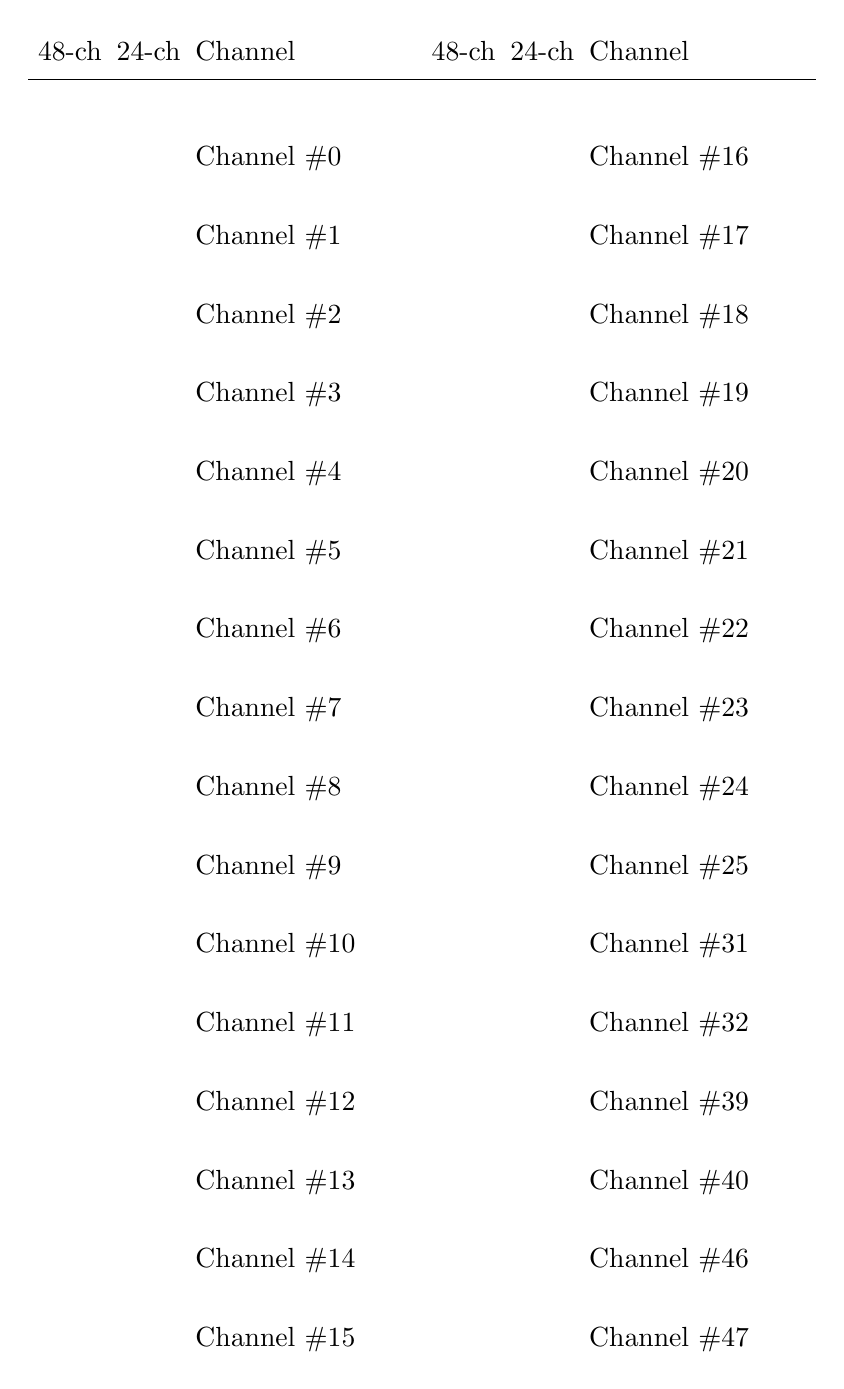
\begin{tikzpicture}
  \node [above right] at (2,11) {\strut Channel};
  \node [above right] at (0,11) {\strut 48-ch};
  \node [above right] at (1,11) {\strut 24-ch};
  \node [above right] at (7,11) {\strut Channel};
  \node [above right] at (5,11) {\strut 48-ch};
  \node [above right] at (6,11) {\strut 24-ch};
  \draw (0,11) -- (10,11);
  \def\y{10}
  \light{A1}{off}\light{G1}{off}\light{Y1}{off}\light{R1}{off}\light{G2}{off}\light{Y2}{off}\light{R2}{sfd}
  \light{A0}{off}\light{G0}{off}\light{Y0}{off}\light{R0}{sfd}
  \node [right] at (2,\y) {Channel \#0};
  \def\y{9}
  \light{A1}{off}\light{G1}{off}\light{Y1}{off}\light{R1}{on}\light{G2}{off}\light{Y2}{off}\light{R2}{sfd}
  \light{A0}{off}\light{G0}{off}\light{Y0}{on}\light{R0}{sfd}
  \node [right] at (2,\y) {Channel \#1};
  \def\y{8}
  \light{A1}{off}\light{G1}{off}\light{Y1}{on}\light{R1}{off}\light{G2}{off}\light{Y2}{off}\light{R2}{sfd}
  \light{A0}{off}\light{G0}{on}\light{Y0}{off}\light{R0}{sfd}
  \node [right] at (2,\y) {Channel \#2};
  \def\y{7}
  \light{A1}{off}\light{G1}{off}\light{Y1}{on}\light{R1}{on}\light{G2}{off}\light{Y2}{off}\light{R2}{sfd}
  \light{A0}{off}\light{G0}{on}\light{Y0}{on}\light{R0}{sfd}
  \node [right] at (2,\y) {Channel \#3};
  \def\y{6}
  \light{A1}{off}\light{G1}{on}\light{Y1}{off}\light{R1}{off}\light{G2}{off}\light{Y2}{off}\light{R2}{sfd}
  \light{A0}{on}\light{G0}{off}\light{Y0}{off}\light{R0}{sfd}
  \node [right] at (2,\y) {Channel \#4};
  \def\y{5}
  \light{A1}{off}\light{G1}{on}\light{Y1}{off}\light{R1}{on}\light{G2}{off}\light{Y2}{off}\light{R2}{sfd}
  \light{A0}{on}\light{G0}{off}\light{Y0}{on}\light{R0}{sfd}
  \node [right] at (2,\y) {Channel \#5};
  \def\y{4}
  \light{A1}{off}\light{G1}{on}\light{Y1}{on}\light{R1}{off}\light{G2}{off}\light{Y2}{off}\light{R2}{sfd}
  \light{A0}{on}\light{G0}{on}\light{Y0}{off}\light{R0}{sfd}
  \node [right] at (2,\y) {Channel \#6};
  \def\y{3}
  \light{A1}{off}\light{G1}{on}\light{Y1}{on}\light{R1}{on}\light{G2}{off}\light{Y2}{off}\light{R2}{sfd}
  \light{A0}{on}\light{G0}{on}\light{Y0}{on}\light{R0}{sfd}
  \node [right] at (2,\y) {Channel \#7};

  \def\y{2}
  \light{A1}{on}\light{G1}{off}\light{Y1}{off}\light{R1}{off}\light{G2}{off}\light{Y2}{off}\light{R2}{sfd}
  \light{A0}{off}\light{G0}{off}\light{Y0}{off}\light{R0}{sfd}
  \node [right] at (2,\y) {Channel \#8};
  \def\y{1}
  \light{A1}{on}\light{G1}{off}\light{Y1}{off}\light{R1}{on}\light{G2}{off}\light{Y2}{off}\light{R2}{sfd}
  \light{A0}{off}\light{G0}{off}\light{Y0}{on}\light{R0}{sfd}
  \node [right] at (2,\y) {Channel \#9};
  \def\y{0}
  \light{A1}{on}\light{G1}{off}\light{Y1}{on}\light{R1}{off}\light{G2}{off}\light{Y2}{off}\light{R2}{sfd}
  \light{A0}{off}\light{G0}{on}\light{Y0}{off}\light{R0}{sfd}
  \node [right] at (2,\y) {Channel \#10};
  \def\y{-1}
  \light{A1}{on}\light{G1}{off}\light{Y1}{on}\light{R1}{on}\light{G2}{off}\light{Y2}{off}\light{R2}{sfd}
  \light{A0}{off}\light{G0}{on}\light{Y0}{on}\light{R0}{sfd}
  \node [right] at (2,\y) {Channel \#11};
  \def\y{-2}
  \light{A1}{on}\light{G1}{on}\light{Y1}{off}\light{R1}{off}\light{G2}{off}\light{Y2}{off}\light{R2}{sfd}
  \light{A0}{on}\light{G0}{off}\light{Y0}{off}\light{R0}{sfd}
  \node [right] at (2,\y) {Channel \#12};
  \def\y{-3}
  \light{A1}{on}\light{G1}{on}\light{Y1}{off}\light{R1}{on}\light{G2}{off}\light{Y2}{off}\light{R2}{sfd}
  \light{A0}{on}\light{G0}{off}\light{Y0}{on}\light{R0}{sfd}
  \node [right] at (2,\y) {Channel \#13};
  \def\y{-4}
  \light{A1}{on}\light{G1}{on}\light{Y1}{on}\light{R1}{off}\light{G2}{off}\light{Y2}{off}\light{R2}{sfd}
  \light{A0}{on}\light{G0}{on}\light{Y0}{off}\light{R0}{sfd}
  \node [right] at (2,\y) {Channel \#14};
  \def\y{-5}
  \light{A1}{on}\light{G1}{on}\light{Y1}{on}\light{R1}{on}\light{G2}{off}\light{Y2}{off}\light{R2}{sfd}
  \light{A0}{on}\light{G0}{on}\light{Y0}{on}\light{R0}{sfd}
  \node [right] at (2,\y) {Channel \#15};

  \def\lightxbase{5}
  \def\y{10}
  \light{A1}{off}\light{G1}{off}\light{Y1}{off}\light{R1}{off}\light{G2}{off}\light{Y2}{on}\light{R2}{sfd}
  \light{A0}{off}\light{G0}{off}\light{Y0}{off}\light{R0}{sfd}
  \node [right] at (7,\y) {Channel \#16};
  \def\y{9}
  \light{A1}{off}\light{G1}{off}\light{Y1}{off}\light{R1}{on}\light{G2}{off}\light{Y2}{on}\light{R2}{sfd}
  \light{A0}{off}\light{G0}{off}\light{Y0}{on}\light{R0}{sfd}
  \node [right] at (7,\y) {Channel \#17};
  \def\y{8}
  \light{A1}{off}\light{G1}{off}\light{Y1}{on}\light{R1}{off}\light{G2}{off}\light{Y2}{on}\light{R2}{sfd}
  \light{A0}{off}\light{G0}{on}\light{Y0}{off}\light{R0}{sfd}
  \node [right] at (7,\y) {Channel \#18};
  \def\y{7}
  \light{A1}{off}\light{G1}{off}\light{Y1}{on}\light{R1}{on}\light{G2}{off}\light{Y2}{on}\light{R2}{sfd}
  \light{A0}{off}\light{G0}{on}\light{Y0}{on}\light{R0}{sfd}
  \node [right] at (7,\y) {Channel \#19};
  \def\y{6}
  \light{A1}{off}\light{G1}{on}\light{Y1}{off}\light{R1}{off}\light{G2}{off}\light{Y2}{on}\light{R2}{sfd}
  \light{A0}{on}\light{G0}{off}\light{Y0}{off}\light{R0}{sfd}
  \node [right] at (7,\y) {Channel \#20};
  \def\y{5}
  \light{A1}{off}\light{G1}{on}\light{Y1}{off}\light{R1}{on}\light{G2}{off}\light{Y2}{on}\light{R2}{sfd}
  \light{A0}{on}\light{G0}{off}\light{Y0}{on}\light{R0}{sfd}
  \node [right] at (7,\y) {Channel \#21};
  \def\y{4}
  \light{A1}{off}\light{G1}{on}\light{Y1}{on}\light{R1}{off}\light{G2}{off}\light{Y2}{on}\light{R2}{sfd}
  \light{A0}{on}\light{G0}{on}\light{Y0}{off}\light{R0}{sfd}
  \node [right] at (7,\y) {Channel \#22};
  \def\y{3}
  \light{A1}{off}\light{G1}{on}\light{Y1}{on}\light{R1}{on}\light{G2}{off}\light{Y2}{on}\light{R2}{sfd}
  \light{A0}{on}\light{G0}{on}\light{Y0}{on}\light{R0}{sfd}
  \node [right] at (7,\y) {Channel \#23};

%         gyAGYR gyAGYR
% 24-31   011000 011111
% 32-39   100000 100111
% 40-47   101000 101111
 
  \def\y{2}
  \light{A1}{on}\light{G1}{off}\light{Y1}{off}\light{R1}{off}\light{G2}{off}\light{Y2}{on}\light{R2}{sfd}
  \node [right] at (7,\y) {Channel \#24};
  \def\y{1}
  \light{A1}{on}\light{G1}{off}\light{Y1}{off}\light{R1}{on}\light{G2}{off}\light{Y2}{on}\light{R2}{sfd}
  \node [right] at (7,\y) {Channel \#25};
  \def\y{0}
  \light{A1}{on}\light{G1}{on}\light{Y1}{on}\light{R1}{on}\light{G2}{off}\light{Y2}{on}\light{R2}{sfd}
  \node [right] at (7,\y) {Channel \#31};
  \def\y{-1}
  \light{A1}{off}\light{G1}{off}\light{Y1}{off}\light{R1}{off}\light{G2}{on}\light{Y2}{off}\light{R2}{sfd}
  \node [right] at (7,\y) {Channel \#32};
  \def\y{-2}
  \light{A1}{off}\light{G1}{on}\light{Y1}{on}\light{R1}{on}\light{G2}{on}\light{Y2}{off}\light{R2}{sfd}
  \node [right] at (7,\y) {Channel \#39};
  \def\y{-3}
  \light{A1}{on}\light{G1}{off}\light{Y1}{off}\light{R1}{off}\light{G2}{on}\light{Y2}{off}\light{R2}{sfd}
  \node [right] at (7,\y) {Channel \#40};
  \def\y{-4}
  \light{A1}{on}\light{G1}{on}\light{Y1}{on}\light{R1}{off}\light{G2}{on}\light{Y2}{off}\light{R2}{sfd}
  \node [right] at (7,\y) {Channel \#46};
  \def\y{-5}
  \light{A1}{on}\light{G1}{on}\light{Y1}{on}\light{R1}{on}\light{G2}{on}\light{Y2}{off}\light{R2}{sfd}
  \node [right] at (7,\y) {Channel \#47};
  \def\lightxbase{0}
    \end{tikzpicture}
  \end{center}
  \caption{Test-mode Channel Indicators\label{fig:testbin}}
\end{figure}

If the \acronym{OPTION} buton is pressed briefly, the pulsing red \acronym{LED} freezes (steady on) and the cycle
pauses on the current output channel.  Pressing the \acronym{OPTION} button again resumes the cycle.
      
\section{Restoring to Factory Settings}\label{ss:factoryreset}
If the board is unresponsive and cannot be reconfigured via the host PC (for example, if you configured
it to use a \ix{baud rate} your host PC can't match), follow these steps to reset the device to its 
factory default settings:
\begin{enumerate}
	\item	Turn off the Lumos controller.
	\item	Disconnect any input sensors and power supply control wire from the Lumos
		controller.
	\item	Install a \ix{jumper} to short pins 4 and 5 of J11 (labeled ``\acronym{ICSP}''
		on the board).
	\item	Power on the Lumos controller.
	\item	When the red, green, and yellow \acronym{LED}s flash rapidly, pull the
		jumper out.
\end{enumerate}

If those steps were carried out exactly as described, %the \acronym{LED}s will all flash rapidly and 
the controller will reboot with the factory settings in place.  This means, among other things,
it will be at address 0, set to use Lumos commands only (not \acronym{DMX512}), and will communicate
at 19,200~baud.

Failure to perform each step at the right time will prevent the factory reset from occurring.

\chapter{Configuring the Board}
\LLstart{T}{here}{are a number of settings} which can be made on the Lumos controllers.  Generally,
this is accomplished by using the \z{lumosctl} com\-mand-line program on the host PC.  The basic configuration
options include such things as setting the device address, communication speed, etc.  These can be set
directly on the command line with \z{lumosctl}.
\index{lumosctl@\z{lumosctl}|(}

In the following examples, the command-line prompt is represented by a `\z{\$}' character.
Text that is typed literally as shown in printed in \z{fixed-width type}, while values which are
to be replaced with a value appropriate for your usage are printed in \Var*{Italics} in angle brackets
(the angle brackets are not actually typed, however).

For every command, you need to include three values:
\begin{itemize}
	\item 	The serial port on the host PC to which the Lumos controller is attached.  This is
		given to \z{lumosctl}'s \z{----port} option, as ``\z{----port=}\Var*{name}''.  On many
		systems, it is enough to say ``\z{----port=0}'' or ``\z{----port=1}'' to specify the first
		or second ``standard'' port.  A specific port name may be given, such as 
		``\z{----port=COM1}'' or ``\z{----port=/dev/ttys0}''.
	\item	The speed (\ix{baud rate}) at which to communicate with the Lumos controller.  This is
		the speed the controller is \emph{currently} using, not the one you want to change it
		to.  This is given as ``\z{----speed=}\Var*{rate}'', such as ``\z{----speed=19200}''.
	\item	The Lumos controller's address, given as ``\z{----address=}\Var*{addr}''.  For example,
		``\z{----addr=0}''.
\end{itemize}

If you aren't sure what device \ix{address}es exist on the serial line, you can have \z{lumosctl} 
probe to discover them all:
\begin{SourceCode}
$ lumosctl --port=COM1 --speed=19200 --probe
Probe discovered 2 devices:
Address 00: lumos48ctl
Address 04: lumos24dc
$ _
\end{SourceCode}

If that doesn't discover everything you thought it should, you can add \z{----verbose} to the command
to see more detail.  Adding more and more \z{----verbose} options increases the amount of information
printed.  The default port is the ``first'' standard port, the default speed is 19,200 bits per second,
and the default address is 0.

If you want to print a full report of the state of a device, include the \z{----report} option:
\begin{SourceCode}
$ lumosctl --port=COM1 --speed=19200 --address=0 --report
\end{SourceCode}

The \z{----port}, \z{----speed}, and \z{----address} options assume a reasonable default value if
they were not specified.  For the sake of simplicity, we'll assume from here on that you either
accept these defaults or are specifying them to have the values you need; we won't explicitly
show them in the examples that follow.

\section{Read-Only Mode}
Sometimes you will use the Lumos board in situations where you can't receive a reply from the device.
This may, for example, happen if you use an \acronym{RS-485} converter which only transmits data, but
doesn't receive any back, or if there is a problem with your PC trying to control the data direction
on a half-duplex network.

In this case, use the \z{----read--only} option to \z{lumosctl}.  This suppresses the features of
\z{lumosctl} which monitor the Lumos board's configuration and current state.  Normally, this helps
confirm that the requested changes took effect, but if your PC is unable to receive information back
from the Lumos board, \z{lumosctl} won't be able to work without the \z{----read-only} option.

\section{Setting the Device Address}
Set a new \ix{address} by giving \z{----set--address=}\Var*{newaddr}.  Don't forget to include the
device's current address with \z{----address=}\Var*{oldaddr}.  For example, to change a board
from address 0 to 12:

\begin{SourceCode}
$ lumosctl --address=0 --set-address=12
\end{SourceCode}

Once the address is set, you'll need to use that value for \z{----address} from that point forward.

\section{Setting the Device Speed}
\index{baud rate}
Set a new speed by giving \z{----set--baud-rate=}\Var*{newspeed}.  Don't forget to include the
device's current speed with \z{----speed=}\Var*{oldspeed}, so it has any hope of seeing the command
to change it.  For example, to change a board
from 19200 to 57600 baud:

\begin{SourceCode}
$ lumosctl --speed=19200 --set-baud-rate=57600
\end{SourceCode}

Once the speed is set, you'll need to use that value for \z{----speed} from that point forward.

\section{Sensors}\label{sec:sensors}

\index{sensors}If your board is built to accommodate sensor inputs, you need to set the \acronym{EEPROM}
settings so the controller stops driving those lines as outputs and starts watching them as
inputs.

To do this, use the \z{----dump--configuration=}\Var*{file} option.  This dumps the device's
configuration state into a text file on the host PC.

\begin{SourceCode}
$ lumosctl --dump-configuration=lumos_board.cfg
\end{SourceCode}

Looking in the \z{lumos\_board.cfg}, find a section beginning with the stanza tag
``\z{[lumos\_device\_settings]}''.
There is a field ``\z{sensors=}\Var*{list}'' which should contain a list of all the sensors 
configured as inputs.  

So if we had lines A and C wired up to sensor inputs instead of \acronym{LED} outputs, we need to 
change this line in the \z{lumos\_board.cfg} file to read:

\begin{SourceCode}
[lumos_device_settings]
sensors=ac
\end{SourceCode}

Leave the other fields alone, just as they are.

\begin{NotImplemented}
For each sensor, we can arrange for an action to take place every time one of them activates.
The actions taken are set up as ``Programmed Sequences'' (see Chapter~\ref{ch:sequences}).
Assuming that the actions we want to carry out are already programmed and loaded as described in
that chapter, we associate those sequences with sensor inputs by introducing a new section
in the \z{lumos\_board.cfg} file called \z{[lumos\_device\_sensor\_}\Var*{x}\z{]}, where 
\Var*{x} is the sensor letter (or we edit that section, if it's already in the file).

For example, to set sensor A to play sequence 100 when it first activates, then continue to loop
sequence 101 as long as the sensor remains active, then finally play sequence 102 as soon as the
sensor stops being active, and assuming we want ``active'' to mean when the signal on that input
is at a logic 1 level (active high), we would put this in the file:

\begin{SourceCode}
[lumos_device_sensor_a]
enabled=yes
mode=while
setup=100
sequence=101
terminate=102
active_low=no
\end{SourceCode}

If we want sensor C to be active low, and trigger sequence 42 one time when it activates, our 
file needs this section added to it:

\begin{SourceCode}
[lumos_device_sensor_c]
enabled=yes
mode=once
sequence=42
active_low=yes
\end{SourceCode}

Once the file is set up with all the configuration changes you wish to make, it may be 
loaded back to the board again with the \z{----load--con\-fig\-ur\-a\-tion=}\Var*{file} option:

\begin{SourceCode}
$ lumosctl --load-configuration=lumos_board.cfg
\end{SourceCode}

Assigning sequences to as sensor-triggered events may also be arranged on the fly via
the \z{lumosctl} program.  The same effects could be performed thus:

\begin{SourceCode}
$ lumosctl --sensor=aw+:100:101:102 --sensor=co::42:
\end{SourceCode}

Note that configuring a sensor line as an input or output \emph{must} be done from the
configuration file.

See Chapter~\ref{ch:sequences} for complete details on how to create sequences and store them
into a Lumos controller.  Full details on the operation of \z{lumosctl} in this and other
areas begins on page~\pageref{ch:lumosctl} in the appendices.
\end{NotImplemented}

\section{Setting a Lumos Controller to Use \acronym{DMX512}}
\begin{NotImplemented*}{The \acronym{DMX512} support in Lumos is experimental and not expected
to work yet.  If you wish to experiment further to refine this feature for a future release of 
the Lumos firmware, contact the author with your findings and recommendations.}
Setting up the controller to be a \acronym{DMX512} device is another task performed via
the configuration file (see Section~\ref{sec:sensors} for instructions about how to dump
and load a configuration file).

First, get the current configuration settings into a file:
\begin{SourceCode}
$ lumosctl --dump-configuration=lumos_board.cfg
\end{SourceCode}
In the \z{[lumos\_device\_settings]} section, add a new field ``\z{dmxchannel=}\Var*{c}'',
where
\Var*{c} is the starting slot number you wish the Lumos controller to use.  This will be 
channel \#0 on this board.  

To cause a 24-channel Lumos board to occupy \acronym*{DMX} slots 200--247, this would be:
\begin{SourceCode}
[lumos_device_settings]
dmxchannel=200
\end{SourceCode}

Now download that configuration into the controller board:
\begin{SourceCode}
$ lumosctl --load-configuration=lumos_board.cfg
\end{SourceCode}

If you want to change the board to be a Lumos-protocol board instead of \acronym{DMX512},
just follow the same process, but \emph{delete} the \z{dmxchannel=}\Var*{c} line completely
before loading the configuration onto the Lumos board.
\end{NotImplemented*}

\section{Canceling Configuration Mode}
When you're finished configuring the controller board, you may use either of these options:
\begin{SourceCode}
$ lumosctl --disable-configuration-mode
$ lumosctl --forbid-configuration-mode
\end{SourceCode}

Either of these returns the board to normal run mode.  The second goes a step further, forbidding
the board from going back into configuration mode again, until the next time the board is reset or
power cycled.
\index{lumosctl@\z{lumosctl}|)}

\chapter{Creating Programmed Sequences}\label{ch:sequences}
\begin{NotImplemented*}{Stored programmed sequences are a planned feature for the Lumos boards but is not
yet implemented.  This chapter will fully describe the programming environment when that feature is
ready for use.}
%% XXX \LLstart{T}{he}{normal operating mode} for a Lumos controller is to receive a stream
%% XXX of real-time commands from the host PC, acting on them as they arrive.  However, it is 
%% XXX also possible to program a number of complex actions into the controller's memory.  The
%% XXX host PC can then send a much smaller command to tell the controller to execute a stored
%% XXX sequence of actions.  If sensor inputs are enabled, the board may be set up to trigger the
%% XXX execution of a stored sequence when sensor activity is detected.
%% XXX 
%% XXX \strong{N.B.: The following information assumes a high-level (if somewhat simple) language
%% XXX to describe sequences, which gets compiled into a more compact bytecode which is loaded onto the
%% XXX device itself.  This language compiler has not yet been written.  Section~\ref{sec:bytecode}
%% XXX below describes the bytecode actually understood by the device.  At the time of this writing,
%% XXX it is necessary to create this bytecode manually and load it into the device as described
%% XXX in that section.  To emphasize that this is speculative documentation about a future feature,
%% XXX the text appears in a lighter type color.}
%% XXX 
%% XXX {\color{gray}
%% XXX These sequences are written using a small, simple programming language.  It is intended to
%% XXX make it possible to describe some basic operations supported by the device, not to create a
%% XXX fully general-purpose programming system.  This, plus the need to design the sequence data
%% XXX to be as compact as possible, drove the design of this language to be optimized toward efficiency
%% XXX and to enable a certain set of common operations.  This optimization means, however, that some
%% XXX other functions are limited or omitted.  We'll point out the major caveats along the way as we
%% XXX describe this system in this chapter.
%% XXX 
%% XXX \section{Basic Sequence Syntax and Structure}
%% XXX Each sequence is numbered with an ID from 0--127.  The sequence begins with a declaration of this
%% XXX ID in the form ``\z{SEQUENCE} \Var*{id}\z{:}'' followed by all the lines of instructions, and ends
%% XXX with the word ``\z{END}'' on the final line.
%% XXX 
%% XXX When writing a sequence of instructions to be stored into the controller, each individual instruction
%% XXX is placed on a line by itself.  For example, if we define sequence~\#1 to set 
%% XXX channel~\#0 on, \#1 to half brightness, and \#2 off,
%% XXX the sequence code would be:
%% XXX \begin{SourceCode}
%% XXX sequence 1:
%% XXX   channel 0 on
%% XXX   channel 1 50%
%% XXX   channel 2 off
%% XXX end
%% XXX \end{SourceCode}
%% XXX % on #0			C1 00
%% XXX % dimmer #1,127		42 01 7F
%% XXX % off #2                41 02
%% XXX 
%% XXX The indentation is simply a convention to make the code more readable; the Lumos system ignores it.
%% XXX Similarly, Lumos sequences are case-insensitive.  The previous sequence could just as well have been
%% XXX written:
%% XXX \begin{SourceCode}
%% XXX SEQUENCE 1:
%% XXX   Channel 0 ON
%% XXX   Channel 1 50%
%% XXX   CHANNEL 2 Off
%% XXX END
%% XXX \end{SourceCode}
%% XXX 
%% XXX \section{Expressions}
%% XXX Anywhere a number is expected, a complex math expression may be used.  Standard algebraic order of
%% XXX operations is enforced on the expression, so parentheses force the enclosed sub-expression to be
%% XXX evaluated first, then multiplication and division, then addition and subtraction.  All of the following
%% XXX instructions turn channel 10 to 1/3 brightness:
%% XXX \begin{SourceCode}
%% XXX channel 10 33.3333333333%
%% XXX channel 2*(2+3) 255/3
%% XXX channel 10 255.0/3.0
%% XXX \end{SourceCode}
%% XXX 
%% XXX \strong{Note:} If the expression is able to be fully interpreted using known values at the time 
%% XXX the source code is compiled on the host PC, it is evaluated with all the precision of floating-point
%% XXX math operations to the extent supported by the PC.  The final result of the calculation, however, 
%% XXX needs to be reduced to (in most cases) an unsigned 8-bit integer value (0--255) for storage on the 
%% XXX Lumos controller.  If the expression must be interpreted at run-time on the Lumos device itself,
%% XXX there's a much more limited expression evaluation system available at that point.  Only addition,
%% XXX subtraction, and multiplication of unsigned 8-bit values is possible there.  The compiler may reject
%% XXX your expression if it can't be handled within those constraints.
%% XXX 
%% XXX The math operators supported are summarized in Figure~\ref{fig:mathop}.
%% XXX \begin{figure}
%% XXX   \begin{center}
%% XXX     \begin{tabular}{|c|l|}\hline
%% XXX 	Expression & Meaning\\\hline\hline
%% XXX 	\Var{x}  \z{+}  \Var{y} & add $x+y$ \\\hline
%% XXX 	\Var{x}  \z{-}  \Var{y} & subtract $x-y$ \\\hline
%% XXX 	\Var{x}  \z{*}  \Var{y} & multiply $x\times y$ \\\hline
%% XXX 	\Var{x}  \z{/}  \Var{y} & divide $x/y$ \\\hline
%% XXX 	\Var{x}  \z{//} \Var{y}& divide $x/y$ using integer division\\\hline
%% XXX 	\Var{x}  \z{\%}  \Var{y}& the remainder when dividing $x/y$ \\\hline
%% XXX     \end{tabular}
%% XXX   \end{center}
%% XXX   \caption{Supported Math Operations\label{fig:mathop}}
%% XXX \end{figure}
%% XXX 
%% XXX \section{Variable Assignment}
%% XXX To a rather limited extent, variables may be defined values and then used in sequences in place
%% XXX of numeric values, like so:
%% XXX \begin{SourceCode}
%% XXX x = 42
%% XXX channel x on
%% XXX channel x+1 on
%% XXX channel x+2 on
%% XXX \end{SourceCode}
%% XXX %
%% XXX % optimized a bit:
%% XXX %
%% XXX % push #42	4F 2A
%% XXX % dup		32
%% XXX % on		81
%% XXX % add		23
%% XXX % dup		32
%% XXX % on		81
%% XXX % add		23
%% XXX % on		81
%% XXX % 
%% XXX % not optimized
%% XXX %
%% XXX % push #42	4F 2A		; SFB+0
%% XXX % push	0	CF 00
%% XXX % on		81
%% XXX % push 	0	CF 00
%% XXX % add		23
%% XXX % on		81
%% XXX % push 	0	CF 00
%% XXX % add	#2	43 02
%% XXX % on		23
%% XXX 
%% XXX \section{Controlling Output Channels}
%% XXX We already saw the \z{CHANNEL} command which can be used to turn a designated channel \z{ON}, 
%% XXX \z{OFF}, or to a given percentage.  It may also be given a raw value from 0--255.  All of the following
%% XXX set channel~\#4 to full brightness:
%% XXX \begin{SourceCode}
%% XXX channel 4 100%
%% XXX channel 4 255
%% XXX cahnnel 4 on
%% XXX \end{SourceCode}
%% XXX 
%% XXX We may also start a channel smoothly fading up or down from its current brightness to either fully
%% XXX on or fully off.  The following instructions cause channel~\#12 to fade to black by reducing its 
%% XXX output value by 2 every .2 seconds.  Simultaneously, channel~\#13 will increase in brightness by 1 step
%% XXX every 1/120\,second.
%% XXX \begin{SourceCode}
%% XXX ramp down 12 by 2 per .2 seconds
%% XXX ramp up 13
%% XXX \end{SourceCode}
%% XXX 
%% XXX There is also a single command for turning all output channels off at once:
%% XXX \begin{SourceCode}
%% XXX blackout
%% XXX \end{SourceCode}
%% XXX 
%% XXX \section{Device State Changes}
%% XXX There are commands \z{SLEEP} and \z{WAKE} to turn on and off sleep mode if desired.
%% XXX These control power-saving features but don't disrupt the interpretation or execution of
%% XXX incoming commands.
%% XXX 
%% XXX There are also \z{SUSPEND} and \z{RESUME} commands.  \z{SUSPEND} causes the controller
%% XXX to ignore any further input, on the premise that the sequence wants to take priority over
%% XXX whatever the host PC wanted the controller to do.  \z{RESUME} allows the board to resume
%% XXX normal operation (acting on received commands from the host PC).
%% XXX 
%% XXX If the command \z{SUSPEND WITH UPDATE} is given, then the device will track changes to
%% XXX channel outputs made by the host PC, but still will not act on them until a \z{RESUME}
%% XXX command (at which point, the output channels will simply change to what would be the
%% XXX final result of all the changes received---it does not ``replay'' all of the changes
%% XXX that were delayed at that point).  
%% XXX 
%% XXX The \z{RESUME WITH FADE} is just like \z{RESUME}, except it will fade all channels to black
%% XXX first, then fade up the channels to their reume values.
%% XXX 
%% XXX For example, if you have a light sensor configured to run sequence 1 once when it senses daylight,
%% XXX and then run sequence 2 when it senses darkness, and you want to inhibit outputs during the daytime
%% XXX but still allow the host PC to set a pattern of channel values which will be displayed immediately
%% XXX upon dusk, the sequences could be coded:
%% XXX \begin{SourceCode}
%% XXX sequence 1:
%% XXX   suspend with update
%% XXX   blackout
%% XXX end
%% XXX 
%% XXX sequence 2:
%% XXX   resume with fade
%% XXX end
%% XXX \end{SourceCode}
%% XXX 
%% XXX \section{Flow Control}
%% XXX In addition to the linear sequence of instructions to change channel outputs, there are
%% XXX a number of instructions which alter the flow of execution itself.  This includes the usual
%% XXX collection including conditionals, loops, and so forth.  
%% XXX 
%% XXX If you want to have sequence 123 turn on channel \#4 if sensor B is active at that moment,
%% XXX or turn it off otherwise, the following code will suffice:
%% XXX \begin{SourceCode}
%% XXX sequence 123:
%% XXX   if sensor b:
%% XXX     channel 4 on
%% XXX   else:
%% XXX     channel 4 off
%% XXX   end
%% XXX end
%% XXX \end{SourceCode}
%% XXX 
%% XXX We can turn on every even numbered channel from \#0--\#10, with a half-second delay up through \#6
%% XXX and then instantly for the rest:
%% XXX \begin{SourceCode}
%% XXX sequence 47:
%% XXX   for ch=0 to 10 by 2:
%% XXX     channel ch on
%% XXX     if channel <= 6:
%% XXX       wait 0.5 seconds
%% XXX     end
%% XXX   end
%% XXX end
%% XXX \end{SourceCode}
%% XXX 
%% XXX We can flash channels \#1 and \#3 repeatedly until our sequence is forced to stop:
%% XXX \begin{SourceCode}
%% XXX sequence 9:
%% XXX   repeat:
%% XXX     channel 1 on
%% XXX     channel 3 on
%% XXX     wait 1 second
%% XXX     channel 1 off
%% XXX     channel 3 off
%% XXX     wait 1 second
%% XXX   end
%% XXX end
%% XXX \end{SourceCode}
%% XXX 
%% XXX Loops can be interrupted using \z{BREAK}, \z{CONTINUE}, and \z{EXIT}.
%% XXX See the \z{lumosctl} documentation (page~\pageref{sh:lumosctl}) for full details.
%% XXX 
%% XXX \section{Subroutines and Sequence Chains}
%% XXX One sequence can invoke another sequence, either as a subroutine (so that the execution
%% XXX temporarily detours into the called sequence, and then the calling sequence resumes where
%% XXX it left off), or as a ``chain'' from one sequence to another (where the calling sequence 
%% XXX stops as the called sequence starts, so there is no returning from that point).
%% XXX 
%% XXX Here we have sequence 12 which calls sequence 13 in a loop:
%% XXX \begin{SourceCode}
%% XXX sequence 12:
%% XXX   repeat 10 times as i:
%% XXX     call 13
%% XXX     wait i seconds
%% XXX   end
%% XXX   execute 14
%% XXX end
%% XXX 
%% XXX sequence 13:
%% XXX   channel 0 on
%% XXX   wait 2
%% XXX   channel 0 off
%% XXX end
%% XXX 
%% XXX sequence 14:
%% XXX   blackout
%% XXX end
%% XXX \end{SourceCode}
%% XXX Note that the \z{EXECUTE} instruction terminated sequence 12 and started
%% XXX sequence 14.  When sequence 14 finishes, nothing further is done.
%% XXX 
%% XXX Sometimes it's valuable to be able to pass parameters to subroutines.  Sequences support
%% XXX up to four parameters which must be declared in both the definition of the sequence and
%% XXX the \z{EXECUTE} or \z{CALL} which invokes it.  Here's a program which turns on each channel
%% XXX from 0--24 repeatedly.
%% XXX \begin{SourceCode}
%% XXX sequence 1:
%% XXX   repeat:
%% XXX     for c=0 to 24:
%% XXX       call 2(c)
%% XXX     end
%% XXX   end
%% XXX end
%% XXX 
%% XXX sequence 2(chan):
%% XXX   channel chan on
%% XXX   wait 1 second
%% XXX   channel chan off
%% XXX end
%% XXX \end{SourceCode}
%% XXX %
%% XXX % 0 loop	0	2A
%% XXX % 1 loop	0	2A
%% XXX % 2 pctr		36
%% XXX % 3 call	$C,#1	48 0C 01
%% XXX % 6 next	1,#24	2B 01 18
%% XXX % 9 next	0	AB 00
%% XXX % b exit		00
%% XXX % c push	0	8F 00
%% XXX % e on			81
%% XXX % f wait	#nn	49 nn
%% XXX %11 push	0	0F 00
%% XXX %13 off			01
%% XXX %14 exit		00
%% XXX 
%% XXX \section{Temporary vs.\ Permanent Sequences}
%% XXX Sequences numbered from 0--63 are stored into non-volatile \acronym{EEPROM} memory and will remain
%% XXX in place until explicitly erased or replaced.  Sequences numbered 64-127 are stored in temporary 
%% XXX \acronym{RAM} and will be lost at the next device reset.  This enables the host PC to download
%% XXX sequences for short-term temporary use.
%% XXX 
%% XXX \section{Storing Sequences into Device Memory}
%% XXX The device files are stored into the Lumos controller using the \z{lumosctl} command:
%% XXX \begin{SourceCode}
%% XXX $ lumosctl --clear-sequences
%% XXX $ lumosctl --load-sequence=my_program_file
%% XXX \end{SourceCode}
%% XXX 
%% XXX The initial \z{----clear--sequences} option is not always needed.  It erases all sequences
%% XXX from memory.  Then each subsequent \z{----load--sequence} option loads a file containing one
%% XXX or more sequences into the device.
%% XXX 
%% XXX If a sequence is loaded which already exists on the device, the old one is replaced with the
%% XXX new one.  Note, however, that Lumos controllers have a very na\"\i ve memory management capability.
%% XXX They are really designed to simply have a set of sequences loaded on them, later erased
%% XXX \emph{en masse} and replaced by a new set.
%% XXX 
%% XXX If replacement sequences are written on top of old ones, it is quite likely that the memory
%% XXX will get fragmented quickly and you'll run out of available memory too early.
%% XXX Simply adding new sequences shouldn't be a problem, however.
%% XXX 
%% XXX You can see how much memory is available by running \z{lumosctl} with the \z{----report} 
%% XXX option.
%% XXX \begin{SourceCode}
%% XXX $ lumosctl --report --address=2
%% XXX ...
%% XXX XXX
%% XXX $ _
%% XXX \end{SourceCode}
%% XXX 
%% XXX \section{Bytecode Reference}\label{sec:bytecode}
%% XXX \emph{This is an advanced reference section most users will never have any reason to 
%% XXX read.}  For the curious, however, we note that when you load a sequence source file
%% XXX into \z{lumosctl}, it compiles the source into bytecode which is what actually gets 
%% XXX sent to the controller, and is what is stored in its memory.  The following reference
%% XXX details the format of that bytecode.
%% XXX 
%% XXX \subsection{Execution Model}
%% XXX The execution model is a small stack-based 
%% XXX \footnote{Several other
%% XXX models were experimented with, but this provided better flexibility with a minimal
%% XXX number of bytes required for the sequence instruction bytes themselves, which need to
%% XXX be stored in a limited space on the controller.} 
%% XXX machine environment, in which
%% XXX each sequence is an independent program which begins at
%% XXX address 0 in its own memory area.  
%% XXX 
%% XXX All memory locations, including program and stacks, are 8~bits wide.  Unless otherwise
%% XXX indicated, data values are unsigned 8-bit integers.
%% XXX 
%% XXX \subsection{Stacks}
%% XXX There are actually three independent stacks used: a call-return stack, data stack, and loop
%% XXX counter stack.
%% XXX 
%% XXX The call-return stack (not illustrated here since it's not directly accessible from your programs) 
%% XXX receives three bytes every time a sequence calls another sequence: the return address, sequence number,
%% XXX and stack frame boundary pointer.
%% XXX %\begin{BF}
%% XXX %  \begin{rightwordgroup}{previous calling sequence}
%% XXX %  \wordbox{1}{return address}\\
%% XXX %  \wordbox{1}{return sequence}\\
%% XXX %  \wordbox{1}{stack frame ptr}
%% XXX %  \end{rightwordgroup}\\
%% XXX %  \begin{rightwordgroup}{calling sequence}
%% XXX %  \wordbox{1}{return address}\\
%% XXX %  \wordbox{1}{return sequence}\\
%% XXX %  \wordbox{1}{stack frame ptr}
%% XXX %  \end{rightwordgroup}\\
%% XXX %  \wordbox[]{1}{$\downarrow$ \\[1ex]}\\
%% XXX %  \wordbox[]{1}{(increasing addresses)}
%% XXX %\end{BF}
%% XXX 
%% XXX We can conceptually picture the stacks as ``piles'' of data values, with the most
%% XXX recently-placed value set on top of the previous ones.  If we ``push'' three values
%% XXX 1, 2, and 3 onto a stack, it would look like this:
%% XXX \begin{center}
%% XXX \begin{bytefield}{8}
%% XXX   \begin{rightwordgroup}{$\leftarrow$Top of Stack}
%% XXX   \wordbox{1}{3}
%% XXX   \end{rightwordgroup}\\
%% XXX   \wordbox{1}{2}\\
%% XXX   \wordbox{1}{1}\\
%% XXX \end{bytefield}
%% XXX \end{center}
%% XXX As we ``pop'' values off the stack, we pull them from the top of the stack, so
%% XXX they are retrieved in the reverse order in which they were pushed onto the
%% XXX stack.
%% XXX 
%% XXX \subsubsection{Loop Counter Stack}
%% XXX The loop counter stack holds all the loop counter values.  %At any given time,
%% XXX %the top of the stack is the counter for the innermost executing loop.  This
%% XXX %value is always referred to as ``\z{\{0\}}'' in the bytecode assembly listings.
%% XXX If the code is executing a nested loop such as:
%% XXX \begin{SourceCode}
%% XXX repeat as outer:
%% XXX   for middle=1 to 10:
%% XXX     repeat 10 as inner:
%% XXX       ...
%% XXX     end
%% XXX   end
%% XXX end
%% XXX \end{SourceCode}
%% XXX 
%% XXX Then the loop stack would look like:
%% XXX \begin{center}
%% XXX \begin{bytefield}[leftcurlyspace=0pt, rightcurlyspace=0pt, leftcurly=., rightcurly=.]{10}
%% XXX   \bitbox[]{2}{} & \bitbox[]{8}{(direction of growth)}\\
%% XXX   \bitbox[]{2}{} & \bitbox[]{8}{$\uparrow$}\\
%% XXX   \bitbox[]{2}{\z{\{0\}}} & \bitbox{8}{\z{inner}}\\
%% XXX   \bitbox[]{2}{\z{\{1\}}} & \bitbox{8}{\z{middle}}\\
%% XXX   \bitbox[]{2}{\z{\{2\}}} & \bitbox{8}{\z{outer}}\\
%% XXX \end{bytefield}
%% XXX \end{center}
%% XXX 
%% XXX At any given time, \z{\{0\}} refers to the top of the loop stack, which is the
%% XXX innermost loop level currently running.  Likewise, \z{\{1\}} is the 
%% XXX counter for the next loop out from there, and so on.
%% XXX 
%% XXX Note that a counter variable is allocated for \emph{every} loop entered,
%% XXX even if the source code didn't associate it with a variable name
%% XXX (e.g., if the innermost was ``\z{REPEAT 10:}'' without the 
%% XXX ``\z{AS INNER}'' part).
%% XXX 
%% XXX \subsubsection{Data Stack}
%% XXX The data stack contains the parameters passed to the current
%% XXX sequence, if any, followed by local variables for the sequence.
%% XXX The remaining room is for working stack space for calculations
%% XXX and values consumed by the opcodes.
%% XXX 
%% XXX At each call, parameters are pushed onto the stack and then the
%% XXX stack frame boundary (\acronym{SFB}) pointer is moved to 
%% XXX point to the first parameter.
%% XXX This way, parameters and local variables are referenced within the
%% XXX sequence as offsets from the frame pointer, while working values
%% XXX are obtained by pushing and popping values from the top of the stack.
%% XXX 
%% XXX \begin{center}
%% XXX \begin{bytefield}{15}%[leftcurlyspace=0pt, rightcurlyspace=0pt, leftcurly=., rightcurly=.]{10}
%% XXX   \begin{leftwordgroup}{Stack Frame}
%% XXX   \begin{rightwordgroup}{working stack}
%% XXX   \bitbox[]{5}{} & \bitbox[]{8}{(increasing addresses)}\\
%% XXX   \bitbox[]{5}{} & \bitbox[]{8}{$\uparrow$}\\
%% XXX   \bitbox[]{5}{\Var{x}} & \bitbox{8}{\Var{d}}\\
%% XXX   \bitbox[]{5}{\Var{y}} & \bitbox{8}{\Var{c}}\\
%% XXX   \bitbox[]{5}{\Var{z}} & \bitbox{8}{\Var{b}}\\
%% XXX   \bitbox[]{5}{}        & \bitbox{8}{\Var{a}}
%% XXX   \end{rightwordgroup}\\
%% XXX   \begin{rightwordgroup}{local variables}
%% XXX   \bitbox[]{5}{\z{[}\Var{n}+\Var{m}--1\z{]}} & \bitbox{8}{\Var{v$_{m-1}$}}\\
%% XXX   \bitbox[]{5}{}        & \bitbox[]{8}{$\vdots$ \\[1ex]}\\
%% XXX   \bitbox[]{5}{\z{[}\Var{n}+1\z{]}} & \bitbox{8}{\Var{v$_1$}}\\
%% XXX   \bitbox[]{5}{\z{[}\Var{n}+0\z{]}} & \bitbox{8}{\Var{v$_0$}}
%% XXX   \end{rightwordgroup}\\
%% XXX   \begin{rightwordgroup}{parameters passed \\ to this sequence}
%% XXX   \bitbox[]{5}{\z{[}\Var{n}--1\z{]}} & \bitbox{8}{\Var{p$_{n-1}$}}\\
%% XXX   \bitbox[]{5}{       } & \bitbox[]{8}{$\vdots$ \\[1ex]}\\
%% XXX   \bitbox[]{5}{\z{[1]}} & \bitbox{8}{\Var{p$_1$}}\\
%% XXX   \bitbox[]{5}{\z{[0]}} & \bitbox{8}{\Var{p$_0$}} & \bitbox[]{2}{$\leftarrow$\acronym{SFB}}
%% XXX   \end{rightwordgroup}
%% XXX   \end{leftwordgroup}\\
%% XXX   %\begin{leftwordgroup}{previous frame}
%% XXX   %\bitbox[]{5}{} &\bitbox{8}{\dots}\\
%% XXX   \bitbox[]{5}{} &\bitbox[]{8}{$\vdots$ \\[1ex]}
%% XXX   %\end{leftwordgroup}\\
%% XXX \end{bytefield}
%% XXX \end{center}
%% XXX 
%% XXX For convenience in our description of the bytecode below, we'll refer to the value on the top of the
%% XXX data stack as \Var{x}, the second value as \Var{y}, and the third as \Var{z}.  In the assembly code,
%% XXX the notation \z{[}\Var{n}\z{]} directly addresses the value \Var{n} bytes from the stack frame boundary
%% XXX (\acronym{SFB}), so the first parameter passed (if any) would be at \z{[0]}, and so on.
%% XXX  
%% XXX \subsection{Instruction Format}
%% XXX 
%% XXX Each instruction is at least one byte long. The first byte is the opcode which always
%% XXX has the general format:
%% XXX %\newcommand\zh{\bitheader{0-7}}
%% XXX \begin{BF}
%% XXX   \bitbox{1}{\Var{f}} & \bitbox{1}{\Var{i}} & \bitbox{1}{\Var{d}} & \bitbox{5}{\Var*{cmd}}
%% XXX \end{BF}
%% XXX Where:
%% XXX \begin{itemize}
%% XXX 	\item[\Var{f}=] Instruction-specific flag.
%% XXX 	\item[\Var{i}=] Data values are given as immediate bytes (\Var{i}=1) instead of being popped
%% XXX 		from the stack (\Var{i}=0).
%% XXX 	\item[\Var{d}=] Take default values for some or all of the arguments (\Var{d}=1).
%% XXX \end{itemize}
%% XXX Note that these are generalizations; individual command opcode patterns vary.
%% XXX 
%% XXX Following the opcode byte are any direct addressing bytes (generally, addresses of locations
%% XXX on the stack for data values, or addresses to jump to) which must be constants at runtime.
%% XXX 
%% XXX After that are zero or more data bytes providing the values needed by the instruction, if the immediate
%% XXX addressing mode is used (bit \Var{i}=1).  Otherwise they will be popped from the data stack as needed.
%% XXX 
%% XXX \subsection{Addressing Modes}
%% XXX The following addressing modes are supported:
%% XXX \begin{itemize}
%% XXX 	\item[--] \emph{Default addressing} means that some or all data values are omitted, 
%% XXX 		(which may be omitted depends on the instruction), so
%% XXX 		the instruction should assume
%% XXX 		a useful default value instead.  Denoted below as either the lack of argument, or
%% XXX 		an explicit mention of the default value (in which case the assembler would convert
%% XXX 		the instruction to the default form and avoid the argument.
%% XXX 	\item[\Var{a}] \emph{Direct addressing} specifies a memory location as a constant value following
%% XXX 		the opcode.  Examples include jump and loop instructions which directly name an
%% XXX 		instruction address within the sequence, and operations which specify a local
%% XXX 		variable or parameter as a constant offset from the stack frame pointer.  Note
%% XXX 		that some instructions mandate a direct argument even if others are pulled from
%% XXX 		the stack, memory, or take defaults.  Denoted below as a number (or name
%% XXX 		defined as a number) without other punctuation.
%% XXX 	\item[\z\#\Var{v}] \emph{Immediate addressing} mode means that the values needed by the instruciton are
%% XXX 		provided as constant bytes following the opcode, rather than being taken from the
%% XXX 		stack.  Denoted below as a value prefixed by a pound sign (\z\#).
%% XXX 	\item[{\z[\Var{a}\z]}] \emph{Indirect addressing} is used when a data value needed by an operation is
%% XXX 		specified, but that value specifies an address in memory (specifically, the value
%% XXX 		is an unsigned integer added to the stack frame pointer).  
%% XXX 		Denoted by square brackets around the argument value.
%% XXX 	\item[{\z{[\$]}}] \emph{Indirect Stack} values are obtained by popping an address from the stack and
%% XXX 		then using it as the location for the value to use.  Noted by square brackets
%% XXX 		and dollar sign together (\z{[\$]}).
%% XXX 	\item[--] \emph{Inherent} means that the instruction simply needs no further values to perform
%% XXX 		its operation; the data is inerent in the instruction itself.
%% XXX 	\item[\z\$] \emph{Stack addressing} means that the data values are popped from the stack.  These are
%% XXX 		popped in the order they would appear if given as immediate bytes, so they would
%% XXX 		need to be pushed in opposite order to that.  Denoted by a dollar sign (\z\$) as
%% XXX 		the argument to the instruction.
%% XXX 	\item[\z\{\Var{v}\z\}] \emph{Loop addressing} accesses loop counter values.  \z{\{0\}} is the
%% XXX 		innermost loop counter (the top of the loop stack), \z{\{1\}} is the next loop out from
%% XXX 		there, etc.  This can be combined with some other modes.  For example, \z{\{\$\}}
%% XXX 		pops a value from the stack, uses that as the loop depth number, and fetches the
%% XXX 		loop counter at that level.
%% XXX \end{itemize}
%% XXX 
%% XXX The addressing mode is selected by various bits in the opcode byte.
%% XXX 
%% XXX For example, the instruction to set the dimmer output level for a channel (mnemonic ``\z{dimmer}'', 
%% XXX base hex opcode \z{0x02}) may have the following forms:
%% XXX 
%% XXX % dimmer #1,16	42 01 10
%% XXX % dimmer 	02
%% XXX % push	 #9	4F 09
%% XXX % push	9	8F 09
%% XXX % push  #0	2F
%% XXX % pctr	2	66 02
%% XXX 
%% XXX \begin{center}
%% XXX \begin{bytefield}[leftcurlyspace=0pt, rightcurlyspace=0pt, leftcurly=., rightcurly=.]{24}
%% XXX 	\bitbox[]{8}{\footnotesize byte 0} &
%% XXX 	\bitbox[]{8}{\footnotesize byte 1} &
%% XXX 	\bitbox[]{8}{\footnotesize byte 2} \\
%% XXX 
%% XXX 	\begin{leftwordgroup}{immed.}
%% XXX 	\begin{rightwordgroup}{\z{dimmer \#1,\#16}}
%% XXX 	\bitbox{1}{\z0} & \bitbox{1}{\z1} & \bitbox{1}{\z0} & \bitbox{5}{\z{0x02}} &
%% XXX 	\bitbox{8}{\z{0x01}} & \bitbox{8}{\z{0x10}}
%% XXX 	\end{leftwordgroup}
%% XXX 	\end{rightwordgroup} \\
%% XXX 
%% XXX 	\begin{leftwordgroup}{stack}
%% XXX 	\begin{rightwordgroup}{\z{dimmer \$,\$}}
%% XXX 	\bitbox{1}{\z0} & \bitbox{1}{\z0} & \bitbox{1}{\z0} & \bitbox{5}{\z{0x02}} &
%% XXX 	\bitbox[]{8}{} & \bitbox[]{8}{}
%% XXX 	\end{leftwordgroup}
%% XXX 	\end{rightwordgroup} \\
%% XXX \end{bytefield}
%% XXX \end{center}
%% XXX 
%% XXX In the first case, the \z{dimmer} command takes the channel number (1) and level (16) as 
%% XXX immediate values in the sequence program itself.  In the second case, it pops two values
%% XXX off the stack, the first number popped being the channel number and the second one being
%% XXX the value.
%% XXX 
%% XXX Consider the \z{push} command as well:
%% XXX 
%% XXX \begin{center}
%% XXX \begin{bytefield}[leftcurlyspace=0pt, rightcurlyspace=0pt, leftcurly=., rightcurly=.]{16}
%% XXX 	\bitbox[]{8}{\footnotesize byte 0} &
%% XXX 	\bitbox[]{8}{\footnotesize byte 1} \\
%% XXX %0F
%% XXX 	\begin{leftwordgroup}{inherent}
%% XXX 	\begin{rightwordgroup}{\z{dup}}
%% XXX 	\bitbox{1}{\z0} & \bitbox{1}{\z0} & \bitbox{1}{\z0} & \bitbox{5}{\z{0x0F}} &
%% XXX 	\bitbox[]{8}{}
%% XXX 	\end{leftwordgroup}
%% XXX 	\end{rightwordgroup}\\
%% XXX %2F
%% XXX 	\begin{leftwordgroup}{default}
%% XXX 	\begin{rightwordgroup}{\z{push \#0}}
%% XXX 	\bitbox{1}{\z0} & \bitbox{1}{\z0} & \bitbox{1}{\z1} & \bitbox{5}{\z{0x0F}} &
%% XXX 	\bitbox[]{8}{}
%% XXX 	\end{leftwordgroup}
%% XXX 	\end{rightwordgroup}\\
%% XXX %4F
%% XXX 	\begin{leftwordgroup}{immediate}
%% XXX 	\begin{rightwordgroup}{\z{push \#9}}
%% XXX 	\bitbox{1}{\z0} & \bitbox{1}{\z1} & \bitbox{1}{\z0} & \bitbox{5}{\z{0x0F}} &
%% XXX 	\bitbox{8}{\z{0x09}}
%% XXX 	\end{leftwordgroup}
%% XXX 	\end{rightwordgroup} \\
%% XXX %6F
%% XXX 	\begin{leftwordgroup}{loop default}
%% XXX 	\begin{rightwordgroup}{\z{push \{0\}}}
%% XXX 	\bitbox{1}{\z0} & \bitbox{1}{\z1} & \bitbox{1}{\z1} & \bitbox{5}{\z{0x0F}} &
%% XXX 	\bitbox[]{8}{}
%% XXX 	\end{leftwordgroup}
%% XXX 	\end{rightwordgroup}\\
%% XXX %8F
%% XXX 	\begin{leftwordgroup}{indirect stack}
%% XXX 	\begin{rightwordgroup}{\z{push [\$]}}
%% XXX 	\bitbox{1}{\z1} & \bitbox{1}{\z0} & \bitbox{1}{\z0} & \bitbox{5}{\z{0x0F}} &
%% XXX 	\bitbox[]{8}{}
%% XXX 	\end{leftwordgroup}
%% XXX 	\end{rightwordgroup}\\
%% XXX %AF
%% XXX 	\begin{leftwordgroup}{indirect default}
%% XXX 	\begin{rightwordgroup}{\z{push [0]}}
%% XXX 	\bitbox{1}{\z1} & \bitbox{1}{\z0} & \bitbox{1}{\z1} & \bitbox{5}{\z{0x0F}} &
%% XXX 	\bitbox[]{8}{}
%% XXX 	\end{leftwordgroup}
%% XXX 	\end{rightwordgroup}\\
%% XXX %CF
%% XXX 	\begin{leftwordgroup}{indirect}
%% XXX 	\begin{rightwordgroup}{\z{push [9]}}
%% XXX 	\bitbox{1}{\z1} & \bitbox{1}{\z1} & \bitbox{1}{\z0} & \bitbox{5}{\z{0x0F}} &
%% XXX 	\bitbox{8}{\z{0x09}}
%% XXX 	\end{leftwordgroup}
%% XXX 	\end{rightwordgroup} \\
%% XXX %EF
%% XXX 	\begin{leftwordgroup}{loop stack}
%% XXX 	\begin{rightwordgroup}{\z{push \{\$\}}}
%% XXX 	\bitbox{1}{\z1} & \bitbox{1}{\z1} & \bitbox{1}{\z1} & \bitbox{5}{\z{0x0F}} &
%% XXX 	\bitbox[]{8}{}
%% XXX 	\end{leftwordgroup}
%% XXX 	\end{rightwordgroup}\\
%% XXX \end{bytefield}
%% XXX \end{center}
%% XXX Some of these combinations are special only for the \z{PUSH} and \z{POP} commands.
%% XXX %, which is the only command
%% XXX %to have eight modes.
%% XXX The first mode is somewhat special as well.  Since ``\z{PUSH \$}'' would
%% XXX not do anything particularly useful---pop a value from the stack and then put it right back 
%% XXX again---this opcode was reassigned to a similar but more useful operation.  Renamed \z{DUP},
%% XXX it takes the value on the top of the stack and pushes another copy of it.
%% XXX 
%% XXX \subsection{Using the Value Stack}
%% XXX The operation of the loop stack and call stack take place behind the scenes where you don't
%% XXX really need to be too concerned about them.  The data stack, on the other hand, is important
%% XXX to understand if you'll be writing sequences at the low level of the bytecodes described here.
%% XXX 
%% XXX The stack has a maximum depth of 256 bytes.  Values are pushed onto it (usually via the \z{PUSH}
%% XXX instruction) and those values are consumed by other instructions as needed.  A \z\$ appearing in
%% XXX an instruction's argument list means to pop a value off the stack for that parameter.
%% XXX 
%% XXX Consider the following sequence of instructions:
%% XXX \begin{SourceCode}
%% XXX base=2
%% XXX for x=1 to 20:
%% XXX   on x
%% XXX   dimmer x+10+base 6*x+12
%% XXX   wait 100
%% XXX   base *= 3
%% XXX end
%% XXX \end{SourceCode}
%% XXX 
%% XXX This would be compiled into the following sequence bytecode:
%% XXX \begin{SourceCode}
%% XXX ADDR BYTES          LINE SOURCE CODE
%% XXX ---- -------------- ---- ------------------------
%% XXX 0000 4F 02          0002      PUSH   #2
%% XXX 0002 AA             0003 L:   LOOP   #1
%% XXX 0003 6F             0004      PUSH   {0}
%% XXX 0004 81             0005      ON     $
%% XXX 0005 6F             0006      PUSH   {0}
%% XXX 0006 52 06          0007      MUL    $,#6
%% XXX 0008 53 0C          0008      ADD    $,#12
%% XXX 000A 6F             0009      PUSH   {0}
%% XXX 000B 53 0A          0010      ADD    $,#10
%% XXX 000D AF             0011      PUSH   [0]
%% XXX 000E 13             0012      ADD    $,$
%% XXX 000F 02             0013      DIMMER $,$
%% XXX 0010 49 64          0014      WAIT   #100
%% XXX 0012 AF             0015      PUSH   [0]
%% XXX 0013 52 03          0016      MUL    $,#3
%% XXX 0015 B0             0017      POP    [0]
%% XXX 0016 6B 02 14       0018      NEXT   L,#1,#20
%% XXX \end{SourceCode}
%% XXX 
%% XXX When executed, this is the sequence of steps carried out, and the stack's contents
%% XXX at each step.  Here's the initial state:
%% XXX 
%% XXX \begin{bytefield}{32}
%% XXX   \bitbox[]{8}{Instruction:} 
%% XXX   & \bitbox[]{2}{} & \bitbox[]{2}{} 
%% XXX   & \bitbox[]{8}{Value Stack:} & \bitbox[]{4}{} 
%% XXX   & \bitbox[]{2}{}
%% XXX   & \bitbox[]{8}{Loop Stack:}\\
%% XXX   \bitbox[]{8}{} 
%% XXX   & \bitbox[]{2}{\z{[0]}} & \bitbox[]{2}{\Var{x}}
%% XXX   & \bitbox{8}{(empty)} & \bitbox[]{4}{$\leftarrow$\acronym{SFB}} 
%% XXX   & \bitbox[]{2}{\z{\{0\}}} & \bitbox{8}{(empty)}
%% XXX \\
%% XXX \end{bytefield}
%% XXX 
%% XXX Now we begin execution.  First, we create a local variable ``\z{base}'' by pushing
%% XXX its initial value (2) onto the stack.  This will be at address zero (relative to the
%% XXX base stack frame pointer), so ``\z{[0]}'' will directly reference this storage location.
%% XXX 
%% XXX \begin{bytefield}{32}
%% XXX   \bitbox[]{8}{\z{PUSH \#2}} 
%% XXX   & \bitbox[]{2}{\z{[0]}} & \bitbox[]{2}{\Var{x}}
%% XXX   & \bitbox{8}{2} & \bitbox[]{4}{$\leftarrow$\acronym{SFB}} 
%% XXX   & \bitbox[]{2}{\z{\{0\}}} & \bitbox{8}{(empty)}
%% XXX \\
%% XXX \end{bytefield}
%% XXX 
%% XXX A new loop context is created with an initial counter value of 1 (now the top of the loop
%% XXX stack).
%% XXX 
%% XXX \begin{bytefield}{32}
%% XXX   \bitbox[]{8}{\z{LOOP \#1}} 
%% XXX   & \bitbox[]{2}{\z{[0]}} & \bitbox[]{2}{\Var{x}}
%% XXX   & \bitbox{8}{2} & \bitbox[]{4}{$\leftarrow$\acronym{SFB}} 
%% XXX   & \bitbox[]{2}{\z{\{0\}}} & \bitbox{8}{1}
%% XXX \\
%% XXX \end{bytefield}
%% XXX 
%% XXX Next we turn on the channel specified by the value of the loop counter, which is on the 
%% XXX loop stack at \z{\{0\}}.  We push that counter onto the data stack then use that as the
%% XXX argument to the \z{ON} instruction.
%% XXX 
%% XXX \begin{bytefield}{32}
%% XXX   \bitbox[]{8}{} 
%% XXX   & \bitbox[]{2}{\z{[1]}} & \bitbox[]{2}{\Var{x}}
%% XXX   & \bitbox{8}{1} & \bitbox[]{4}{}
%% XXX   & \bitbox[]{2}{} & \bitbox[]{8}{}
%% XXX \\
%% XXX   \bitbox[]{8}{\z{PUSH \{0\}}} 
%% XXX   & \bitbox[]{2}{\z{[0]}} & \bitbox[]{2}{\Var{y}}
%% XXX   & \bitbox{8}{2} & \bitbox[]{4}{$\leftarrow$\acronym{SFB}} 
%% XXX   & \bitbox[]{2}{\z{\{0\}}} & \bitbox{8}{1}
%% XXX \\
%% XXX \end{bytefield}
%% XXX 
%% XXX Since the value at the top of the stack (\Var{x}) is~1, the
%% XXX instruction \z{ON \$} pops that value and turns on channel~1.
%% XXX 
%% XXX \begin{bytefield}{32}
%% XXX   \bitbox[]{8}{\z{ON \$}} 
%% XXX   & \bitbox[]{2}{\z{[0]}} & \bitbox[]{2}{\Var{x}}
%% XXX   & \bitbox{8}{2} & \bitbox[]{4}{$\leftarrow$\acronym{SFB}} 
%% XXX   & \bitbox[]{2}{\z{\{0\}}} & \bitbox{8}{1}
%% XXX \\
%% XXX \end{bytefield}
%% XXX 
%% XXX Now we need to evaluate \z{6*x+12}.
%% XXX 
%% XXX \begin{bytefield}{32}
%% XXX   \bitbox[]{8}{} 
%% XXX   & \bitbox[]{2}{\z{[1]}} & \bitbox[]{2}{\Var{x}}
%% XXX   & \bitbox{8}{1} & \bitbox[]{4}{}
%% XXX   & \bitbox[]{2}{} & \bitbox[]{8}{}
%% XXX \\
%% XXX   \bitbox[]{8}{\z{PUSH \{0\}}} 
%% XXX   & \bitbox[]{2}{\z{[0]}} & \bitbox[]{2}{\Var{y}}
%% XXX   & \bitbox{8}{2} & \bitbox[]{4}{$\leftarrow$\acronym{SFB}} 
%% XXX   & \bitbox[]{2}{\z{\{0\}}} & \bitbox{8}{1}
%% XXX \\
%% XXX \end{bytefield}
%% XXX 
%% XXX The 1 on the top of the stack is popped off, multiplied by 6, and the
%% XXX product pushed back onto the stack:
%% XXX 
%% XXX \begin{bytefield}{32}
%% XXX   \bitbox[]{8}{} 
%% XXX   & \bitbox[]{2}{\z{[1]}} & \bitbox[]{2}{\Var{x}}
%% XXX   & \bitbox{8}{6} & \bitbox[]{4}{}
%% XXX   & \bitbox[]{2}{} & \bitbox[]{8}{}
%% XXX \\
%% XXX   \bitbox[]{8}{\z{MUL \$,\#6}} 
%% XXX   & \bitbox[]{2}{\z{[0]}} & \bitbox[]{2}{\Var{y}}
%% XXX   & \bitbox{8}{2} & \bitbox[]{4}{$\leftarrow$\acronym{SFB}} 
%% XXX   & \bitbox[]{2}{\z{\{0\}}} & \bitbox{8}{1}
%% XXX \\
%% XXX \end{bytefield}
%% XXX   
%% XXX The product is popped, added to 12 and the sum pushed back:
%% XXX 
%% XXX \begin{bytefield}{32}
%% XXX   \bitbox[]{8}{} 
%% XXX   & \bitbox[]{2}{\z{[1]}} & \bitbox[]{2}{\Var{x}}
%% XXX   & \bitbox{8}{18} & \bitbox[]{4}{}
%% XXX   & \bitbox[]{2}{} & \bitbox[]{8}{}
%% XXX \\
%% XXX   \bitbox[]{8}{\z{ADD \$,\#12}} 
%% XXX   & \bitbox[]{2}{\z{[0]}} & \bitbox[]{2}{\Var{y}}
%% XXX   & \bitbox{8}{2} & \bitbox[]{4}{$\leftarrow$\acronym{SFB}} 
%% XXX   & \bitbox[]{2}{\z{\{0\}}} & \bitbox{8}{1}
%% XXX \\
%% XXX \end{bytefield}
%% XXX 
%% XXX Now that we have the value to be set on the channel (18),
%% XXX we calculate the channel number as \z{x+10+base}:
%% XXX 
%% XXX \begin{bytefield}{32}
%% XXX   \bitbox[]{8}{} 
%% XXX   & \bitbox[]{2}{\z{[2]}} & \bitbox[]{2}{\Var{x}}
%% XXX   & \bitbox{8}{1} & \bitbox[]{4}{}
%% XXX   & \bitbox[]{2}{} & \bitbox[]{8}{}
%% XXX \\
%% XXX   \bitbox[]{8}{} 
%% XXX   & \bitbox[]{2}{\z{[1]}} & \bitbox[]{2}{\Var{y}}
%% XXX   & \bitbox{8}{18} & \bitbox[]{4}{}
%% XXX   & \bitbox[]{2}{} & \bitbox[]{8}{}
%% XXX \\
%% XXX   \bitbox[]{8}{\z{PUSH \{0\}}} 
%% XXX   & \bitbox[]{2}{\z{[0]}} & \bitbox[]{2}{\Var{z}}
%% XXX   & \bitbox{8}{2} & \bitbox[]{4}{$\leftarrow$\acronym{SFB}} 
%% XXX   & \bitbox[]{2}{\z{\{0\}}} & \bitbox{8}{1}
%% XXX \\
%% XXX \end{bytefield}
%% XXX 
%% XXX \begin{bytefield}{32}
%% XXX   \bitbox[]{8}{} 
%% XXX   & \bitbox[]{2}{\z{[2]}} & \bitbox[]{2}{\Var{x}}
%% XXX   & \bitbox{8}{11} & \bitbox[]{4}{}
%% XXX   & \bitbox[]{2}{} & \bitbox[]{8}{}
%% XXX \\
%% XXX   \bitbox[]{8}{} 
%% XXX   & \bitbox[]{2}{\z{[1]}} & \bitbox[]{2}{\Var{y}}
%% XXX   & \bitbox{8}{18} & \bitbox[]{4}{}
%% XXX   & \bitbox[]{2}{} & \bitbox[]{8}{}
%% XXX \\
%% XXX   \bitbox[]{8}{\z{ADD \$,\#10}} 
%% XXX   & \bitbox[]{2}{\z{[0]}} & \bitbox[]{2}{\Var{z}}
%% XXX   & \bitbox{8}{2} & \bitbox[]{4}{$\leftarrow$\acronym{SFB}} 
%% XXX   & \bitbox[]{2}{\z{\{0\}}} & \bitbox{8}{1}
%% XXX \\
%% XXX \end{bytefield}
%% XXX 
%% XXX The value of the local variable \z{base} is at local address
%% XXX 0 (i.e., \acronym{SFB}+0, also known as ``\z{[0]}''), so we push that onto
%% XXX the stack then add it to our sum.
%% XXX 
%% XXX \begin{bytefield}{32}
%% XXX   \bitbox[]{8}{} 
%% XXX   & \bitbox[]{2}{\z{[3]}} & \bitbox[]{2}{\Var{x}}
%% XXX   & \bitbox{8}{2} & \bitbox[]{4}{}
%% XXX   & \bitbox[]{2}{} & \bitbox[]{8}{}
%% XXX \\
%% XXX   \bitbox[]{8}{} 
%% XXX   & \bitbox[]{2}{\z{[2]}} & \bitbox[]{2}{\Var{y}}
%% XXX   & \bitbox{8}{11} & \bitbox[]{4}{}
%% XXX   & \bitbox[]{2}{} & \bitbox[]{8}{}
%% XXX \\
%% XXX   \bitbox[]{8}{} 
%% XXX   & \bitbox[]{2}{\z{[1]}} & \bitbox[]{2}{\Var{z}}
%% XXX   & \bitbox{8}{18} & \bitbox[]{4}{}
%% XXX   & \bitbox[]{2}{} & \bitbox[]{8}{}
%% XXX \\
%% XXX   \bitbox[]{8}{\z{PUSH [0]}} 
%% XXX   & \bitbox[]{2}{\z{[0]}} & \bitbox[]{2}{}
%% XXX   & \bitbox{8}{2} & \bitbox[]{4}{$\leftarrow$\acronym{SFB}} 
%% XXX   & \bitbox[]{2}{\z{\{0\}}} & \bitbox{8}{1}
%% XXX \\
%% XXX \end{bytefield}
%% XXX 
%% XXX \begin{bytefield}{32}
%% XXX   \bitbox[]{8}{} 
%% XXX   & \bitbox[]{2}{\z{[2]}} & \bitbox[]{2}{\Var{x}}
%% XXX   & \bitbox{8}{13} & \bitbox[]{4}{}
%% XXX   & \bitbox[]{2}{} & \bitbox[]{8}{}
%% XXX \\
%% XXX   \bitbox[]{8}{} 
%% XXX   & \bitbox[]{2}{\z{[1]}} & \bitbox[]{2}{\Var{y}}
%% XXX   & \bitbox{8}{18} & \bitbox[]{4}{}
%% XXX   & \bitbox[]{2}{} & \bitbox[]{8}{}
%% XXX \\
%% XXX   \bitbox[]{8}{\z{ADD \$,\$}} 
%% XXX   & \bitbox[]{2}{\z{[0]}} & \bitbox[]{2}{\Var{z}}
%% XXX   & \bitbox{8}{2} & \bitbox[]{4}{$\leftarrow$\acronym{SFB}} 
%% XXX   & \bitbox[]{2}{\z{\{0\}}} & \bitbox{8}{1}
%% XXX \\
%% XXX \end{bytefield}
%% XXX 
%% XXX Now we pop the channel number and level off the stack
%% XXX so channel~13 is set to dimmer level~18.
%% XXX 
%% XXX \begin{bytefield}{32}
%% XXX   \bitbox[]{8}{\z{DIMMER \$,\$}} 
%% XXX   & \bitbox[]{2}{\z{[0]}} & \bitbox[]{2}{\Var{x}}
%% XXX   & \bitbox{8}{2} & \bitbox[]{4}{$\leftarrow$\acronym{SFB}} 
%% XXX   & \bitbox[]{2}{\z{\{0\}}} & \bitbox{8}{1}
%% XXX \\
%% XXX \end{bytefield}
%% XXX 
%% XXX Now we wait, which doesn't affect the stack.
%% XXX 
%% XXX \begin{bytefield}{32}
%% XXX   \bitbox[]{8}{\z{WAIT \#100}} 
%% XXX   & \bitbox[]{2}{\z{[0]}} & \bitbox[]{2}{\Var{x}}
%% XXX   & \bitbox{8}{2} & \bitbox[]{4}{$\leftarrow$\acronym{SFB}} 
%% XXX   & \bitbox[]{2}{\z{\{0\}}} & \bitbox{8}{1}
%% XXX \\
%% XXX \end{bytefield}
%% XXX 
%% XXX To update the value of the variable \z{base}, we push its
%% XXX current value from memory location \z{[0]}, multiply it by 3
%% XXX to get the new value, and the pop that result back into 
%% XXX memory location \z{[0]} again.\footnote{``Wait a moment,'' you may be asking yourself
%% XXX at this point, ``The value of \z{base} is sitting \emph{right there} on the stack,
%% XXX why not just execute the single instruction \z{MUL \#3} and accomplish the same
%% XXX thing in one step?'' The answer is that you can, in this particular case.  In some sequences,
%% XXX though, there may be other variables in the way, so the approach outlined here will
%% XXX work in the general case.  If you're hand-compiling your own bytecode, you can make
%% XXX optimizations like that.}
%% XXX 
%% XXX \begin{bytefield}{32}
%% XXX   \bitbox[]{8}{} 
%% XXX   & \bitbox[]{2}{\z{[1]}} & \bitbox[]{2}{\Var{x}}
%% XXX   & \bitbox{8}{2} & \bitbox[]{4}{}
%% XXX   & \bitbox[]{2}{} & \bitbox[]{8}{}
%% XXX \\
%% XXX   \bitbox[]{8}{\z{PUSH [0]}} 
%% XXX   & \bitbox[]{2}{\z{[0]}} & \bitbox[]{2}{\Var{y}}
%% XXX   & \bitbox{8}{2} & \bitbox[]{4}{$\leftarrow$\acronym{SFB}} 
%% XXX   & \bitbox[]{2}{\z{\{0\}}} & \bitbox{8}{1}
%% XXX \\
%% XXX \end{bytefield}
%% XXX   
%% XXX \begin{bytefield}{32}
%% XXX   \bitbox[]{8}{} 
%% XXX   & \bitbox[]{2}{\z{[1]}} & \bitbox[]{2}{\Var{x}}
%% XXX   & \bitbox{8}{6} & \bitbox[]{4}{}
%% XXX   & \bitbox[]{2}{} & \bitbox[]{8}{}
%% XXX \\
%% XXX   \bitbox[]{8}{\z{MUL \$,\#3}} 
%% XXX   & \bitbox[]{2}{\z{[0]}} & \bitbox[]{2}{\Var{y}}
%% XXX   & \bitbox{8}{2} & \bitbox[]{4}{$\leftarrow$\acronym{SFB}} 
%% XXX   & \bitbox[]{2}{\z{\{0\}}} & \bitbox{8}{1}
%% XXX \\
%% XXX \end{bytefield}
%% XXX   
%% XXX \begin{bytefield}{32}
%% XXX   \bitbox[]{8}{\z{POP [0]}} 
%% XXX   & \bitbox[]{2}{\z{[0]}} & \bitbox[]{2}{\Var{x}}
%% XXX   & \bitbox{8}{6} & \bitbox[]{4}{$\leftarrow$\acronym{SFB}} 
%% XXX   & \bitbox[]{2}{\z{\{0\}}} & \bitbox{8}{1}
%% XXX \\
%% XXX \end{bytefield}
%% XXX   
%% XXX We then start the next iteration.
%% XXX 
%% XXX \begin{bytefield}{32}
%% XXX   \bitbox[]{8}{\z{NEXT L,\#1,\#20}} 
%% XXX   & \bitbox[]{2}{\z{[0]}} & \bitbox[]{2}{\Var{x}}
%% XXX   & \bitbox{8}{6} & \bitbox[]{4}{$\leftarrow$\acronym{SFB}} 
%% XXX   & \bitbox[]{2}{\z{\{0\}}} & \bitbox{8}{2}
%% XXX \\
%% XXX \end{bytefield}
%% XXX 
%% XXX \dots\ and so on, until we reach the end of the final iteration:
%% XXX 
%% XXX \begin{bytefield}{32}
%% XXX   \bitbox[]{8}{\z{}}
%% XXX   & \bitbox[]{2}{\z{[0]}} & \bitbox[]{2}{\Var{x}}
%% XXX   & \bitbox{8}{34} & \bitbox[]{4}{$\leftarrow$\acronym{SFB}} 
%% XXX   & \bitbox[]{2}{\z{\{0\}}} & \bitbox{8}{20}
%% XXX \\
%% XXX \end{bytefield}
%% XXX 
%% XXX (Note that the value in \z{[0]}---the local variable ``\z{base}''---is multiplied
%% XXX by 3$\times$ every iteration, so although the value in the 8-bit memory location is
%% XXX currently 34, it's overflowed 13~times already.  Remember that you are working with
%% XXX only 8-bit values on the Lumos device.)
%% XXX 
%% XXX When the \z{NEXT} instruction is executed, it determines that the loop exit
%% XXX condition has been met, and destroys the loop context, does \emph{not} jump to
%% XXX the top of the loop, and execution will continue on past the loop now.
%% XXX 
%% XXX \begin{bytefield}{32}
%% XXX   \bitbox[]{8}{\z{NEXT 2,\#1,\#20}} 
%% XXX   & \bitbox[]{2}{\z{[0]}} & \bitbox[]{2}{\Var{x}}
%% XXX   & \bitbox{8}{34} & \bitbox[]{4}{$\leftarrow$\acronym{SFB}} 
%% XXX   & \bitbox[]{2}{\z{\{0\}}} & \bitbox{8}{(empty)}
%% XXX \\
%% XXX \end{bytefield}
%% XXX 
%% XXX \subsection{Subroutine Calls and Parameter Passing}
%% XXX The basic unit of execution is a sequence itself, so when we speak of calling a ``subroutine''
%% XXX we really mean one sequence is calling another sequence (or recursively calling itself).
%% XXX 
%% XXX A number of parameters may be passed to the called sequence, which will appear as local
%% XXX variables to it.  This is done by pushing their values onto the stack before making the
%% XXX call.  Part of the call itself moves the stack frame boundary so that location \z{[0]}
%% XXX refers to the first parameter.  The other parameters, if any, follow.  If the called
%% XXX sequence sets up local variables, they'll be pushed after the parameters (which means
%% XXX it is important that the sequences all agree about how many parameters are being passed
%% XXX and received).
%% XXX 
%% XXX To illustrate this, consider the following pair of sequences:
%% XXX 
%% XXX \begin{SourceCode}
%% XXX sequence 1:
%% XXX   delay=10
%% XXX   for i=0 to 255 by 4:
%% XXX     for j=20 to 10 by -1:
%% XXX       call 5(i,j)
%% XXX       wait delay
%% XXX     end
%% XXX     delay += 10
%% XXX   end
%% XXX end
%% XXX  
%% XXX sequence 5(val,ch):
%% XXX   foo=0x42
%% XXX   dimmer ch, val
%% XXX   on ch+20
%% XXX   off ch+20
%% XXX end
%% XXX \end{SourceCode}
%% XXX 
%% XXX This compiles into the following bytecode:
%% XXX 
%% XXX \label{src:2seq}
%% XXX \begin{SourceCode}
%% XXX SEQUENCE #1 ASSEMBLY LISTING
%% XXX ADDR BYTES          LINE SOURCE CODE
%% XXX ---- -------------- ---- -----------------------------
%% XXX 0000 4F 0A          0002 	PUSH    #10
%% XXX 0002 2A             0003 I_LOOP: LOOP    #0
%% XXX 0003 4A 14          0004 J_LOOP:	LOOP    #20
%% XXX 0005 4F 01          0005 	PUSH    #1
%% XXX 0007 EF             0006 	PUSH    {$}
%% XXX 0008 6F             0007 	PUSH    {0}
%% XXX 0009 48 05 02       0008 	CALL    #5,#2
%% XXX 000C AF             0009 	PUSH    [0]
%% XXX 000D 09             0010 	WAIT    $
%% XXX 000E 75 03 0A       0011 	NEXTDEC J_LOOP,#1,#10
%% XXX 0011 AF             0012 	PUSH    [0]
%% XXX 0012 53 0A          0013 	ADD     $,#10
%% XXX 0014 B0             0014 	POP     [0]
%% XXX 0015 4B 02 04 FF    0015 	NEXT    I_LOOP,#4,#255
%% XXX 0019 00             0016 	EXIT
%% XXX 
%% XXX SEQUENCE #5 ASSEMBLY LISTING
%% XXX ADDR BYTES          LINE SOURCE CODE
%% XXX ---- -------------- ---- -----------------------------
%% XXX 0000 40 02          0019 	SSFB    #2
%% XXX 0002 4F 42          0020 	PUSH    #0x42
%% XXX 0004 AF             0021 	PUSH    [0]
%% XXX 0005 CF 01          0022 	PUSH    [1]
%% XXX 0007 02             0023 	DIMMER  $,$
%% XXX 0008 CF 01          0024 	PUSH    [1]
%% XXX 000A 53 14          0025 	ADD     $,#20
%% XXX 000C 0F             0026 	DUP
%% XXX 000D 81             0027 	ON      $
%% XXX 000E 01             0028 	OFF     $
%% XXX 000F 00             0029 	EXIT
%% XXX \end{SourceCode}
%% XXX 
%% XXX We'll step through the execution of these routines to show how the stack frames
%% XXX look between calls.
%% XXX 
%% XXX First, sequence~1 starts running, pushes its local variable to the stack, and enters
%% XXX its loops:
%% XXX 
%% XXX \begin{bytefield}{32}
%% XXX   \bitbox[]{8}{\z{PUSH \#10}} 
%% XXX   & \bitbox[]{2}{\z{[0]}} & \bitbox[]{2}{\Var{x}}
%% XXX   & \bitbox{8}{10} & \bitbox[]{4}{$\leftarrow$\acronym{SFB}} 
%% XXX   & \bitbox[]{2}{\z{\{0\}}} & \bitbox{8}{(empty)}
%% XXX \\
%% XXX \end{bytefield}
%% XXX 
%% XXX \begin{bytefield}{32}
%% XXX   \bitbox[]{8}{\z{LOOP \#0}} 
%% XXX   & \bitbox[]{2}{\z{[0]}} & \bitbox[]{2}{\Var{x}}
%% XXX   & \bitbox{8}{10} & \bitbox[]{4}{$\leftarrow$\acronym{SFB}} 
%% XXX   & \bitbox[]{2}{\z{\{0\}}} & \bitbox{8}{0}
%% XXX \\
%% XXX \end{bytefield}
%% XXX 
%% XXX \begin{bytefield}{32}
%% XXX   \bitbox[]{8}{}
%% XXX   & \bitbox[]{2}{} & \bitbox[]{2}{}
%% XXX   & \bitbox[]{8}{} & \bitbox[]{4}{}
%% XXX   & \bitbox[]{2}{\z{\{0\}}} & \bitbox{8}{20}
%% XXX \\
%% XXX   \bitbox[]{8}{\z{LOOP \#20}} 
%% XXX   & \bitbox[]{2}{\z{[0]}} & \bitbox[]{2}{\Var{x}}
%% XXX   & \bitbox{8}{10} & \bitbox[]{4}{$\leftarrow$\acronym{SFB}} 
%% XXX   & \bitbox[]{2}{\z{\{1\}}} & \bitbox{8}{0}
%% XXX \\
%% XXX \end{bytefield}
%% XXX 
%% XXX We push the two parameters onto the stack in the order shown in the source code
%% XXX (i.e., the deepest value will be the first parameter).  Since the call is
%% XXX ``\z{CALL 5(x,y)}'' we need to push the outer loop counter \z{x} (which is 
%% XXX at position \z{\{1\}} on the loop stack), then the inner loop counter \z{y}
%% XXX (which is at position \z{\{0\}}).
%% XXX 
%% XXX \begin{bytefield}{32}
%% XXX   \bitbox[]{8}{}
%% XXX   & \bitbox[]{2}{\z{[1]}} & \bitbox[]{2}{\Var{x}}
%% XXX   & \bitbox{8}{1} & \bitbox[]{4}{}
%% XXX   & \bitbox[]{2}{\z{\{0\}}} & \bitbox{8}{20}
%% XXX \\
%% XXX   \bitbox[]{8}{\z{PUSH \#1}}
%% XXX   & \bitbox[]{2}{\z{[0]}} & \bitbox[]{2}{\Var{y}}
%% XXX   & \bitbox{8}{10} & \bitbox[]{4}{$\leftarrow$\acronym{SFB}} 
%% XXX   & \bitbox[]{2}{\z{\{1\}}} & \bitbox{8}{0}
%% XXX \\
%% XXX \end{bytefield}
%% XXX 
%% XXX \begin{bytefield}{32}
%% XXX   \bitbox[]{8}{}
%% XXX   & \bitbox[]{2}{\z{[1]}} & \bitbox[]{2}{\Var{x}}
%% XXX   & \bitbox{8}{0} & \bitbox[]{4}{}
%% XXX   & \bitbox[]{2}{\z{\{0\}}} & \bitbox{8}{20}
%% XXX \\
%% XXX   \bitbox[]{8}{\z{PUSH \{\$\}}}
%% XXX   & \bitbox[]{2}{\z{[0]}} & \bitbox[]{2}{\Var{y}}
%% XXX   & \bitbox{8}{10} & \bitbox[]{4}{$\leftarrow$\acronym{SFB}} 
%% XXX   & \bitbox[]{2}{\z{\{1\}}} & \bitbox{8}{0}
%% XXX \\
%% XXX \end{bytefield}
%% XXX 
%% XXX \begin{bytefield}{32}
%% XXX   \bitbox[]{8}{}
%% XXX   & \bitbox[]{2}{\z{[2]}} & \bitbox[]{2}{\Var{x}}
%% XXX   & \bitbox{8}{20} & \bitbox[]{4}{}
%% XXX   & \bitbox[]{2}{} & \bitbox[]{8}{}
%% XXX \\
%% XXX   \bitbox[]{8}{}
%% XXX   & \bitbox[]{2}{\z{[1]}} & \bitbox[]{2}{\Var{y}}
%% XXX   & \bitbox{8}{0} & \bitbox[]{4}{}
%% XXX   & \bitbox[]{2}{\z{\{0\}}} & \bitbox{8}{20}
%% XXX \\
%% XXX   \bitbox[]{8}{\z{PUSH \{0\}}}
%% XXX   & \bitbox[]{2}{\z{[0]}} & \bitbox[]{2}{\Var{z}}
%% XXX   & \bitbox{8}{10} & \bitbox[]{4}{$\leftarrow$\acronym{SFB}} 
%% XXX   & \bitbox[]{2}{\z{\{1\}}} & \bitbox{8}{0}
%% XXX \\
%% XXX \end{bytefield}
%% XXX 
%% XXX Now we make the call.  The first parameter to \z{CALL} is the sequence number
%% XXX we're calling, and the second is the number of parameters being passed (2 in this
%% XXX case).
%% XXX 
%% XXX \begin{bytefield}{32}
%% XXX   \bitbox[]{8}{}
%% XXX   & \bitbox[]{2}{\z{[1]}} & \bitbox[]{2}{\Var{x}}
%% XXX   & \bitbox{8}{20} & \bitbox[]{4}{}
%% XXX   & \bitbox[]{2}{} & \bitbox[]{8}{}
%% XXX \\
%% XXX   \bitbox[]{8}{}
%% XXX   & \bitbox[]{2}{\z{[0]}} & \bitbox[]{2}{\Var{y}}
%% XXX   & \bitbox{8}{0} & \bitbox[]{4}{$\leftarrow$\acronym{SFB}}
%% XXX   & \bitbox[]{2}{\z{\{0\}}} & \bitbox{8}{20}
%% XXX \\
%% XXX   \bitbox[]{8}{\z{CALL \#5,\#2}}
%% XXX   & \bitbox[]{2}{} & \bitbox[]{2}{}
%% XXX   & \colorbitbox{lightgray}{8}{10} & \bitbox[]{4}{} 
%% XXX   & \bitbox[]{2}{\z{\{1\}}} & \bitbox{8}{0}
%% XXX \\
%% XXX \end{bytefield}
%% XXX 
%% XXX At this point, control transfers into sequence~5.  Note that the stack frame boundary
%% XXX moved up until the frame includes only the top 2 items (the two parameters passed into 
%% XXX this sequence).  This means the parameters are directly accessible as \z{[0]}
%% XXX and \z{[1]}, and the local variable sequence~5 is about to create will be \z{[2]}.  The
%% XXX local variable from the calling sequence (the value 10 on the stack) is not directly
%% XXX accessible for now.\footnote{Yes, if you're clever or careless enough, you can destroy
%% XXX the integrity of the stack(s) to retrieve or alter the values below \acronym{SFB}, but
%% XXX we're not recommending that.}
%% XXX 
%% XXX The first thing sequence~5 does is to ensure the stack frame is as expected.  
%% XXX 
%% XXX \begin{bytefield}{32}
%% XXX   \bitbox[]{8}{}
%% XXX   & \bitbox[]{2}{\z{[1]}} & \bitbox[]{2}{\Var{x}}
%% XXX   & \bitbox{8}{20} & \bitbox[]{4}{}
%% XXX   & \bitbox[]{2}{} & \bitbox[]{8}{}
%% XXX \\
%% XXX   \bitbox[]{8}{}
%% XXX   & \bitbox[]{2}{\z{[0]}} & \bitbox[]{2}{\Var{y}}
%% XXX   & \bitbox{8}{0} & \bitbox[]{4}{$\leftarrow$\acronym{SFB}}
%% XXX   & \bitbox[]{2}{\z{\{0\}}} & \bitbox{8}{20}
%% XXX \\
%% XXX   \bitbox[]{8}{\z{SSFB \#2}}
%% XXX   & \bitbox[]{2}{} & \bitbox[]{2}{}
%% XXX   & \colorbitbox{lightgray}{8}{10} & \bitbox[]{4}{} 
%% XXX   & \bitbox[]{2}{\z{\{1\}}} & \bitbox{8}{0}
%% XXX \\
%% XXX \end{bytefield}
%% XXX 
%% XXX Next, it will
%% XXX push the initial value of the local variable
%% XXX \z{foo}, so we can get to it at location \z{[2]}.
%% XXX 
%% XXX \begin{bytefield}{32}
%% XXX   \bitbox[]{8}{}
%% XXX   & \bitbox[]{2}{\z{[2]}} & \bitbox[]{2}{\Var{x}}
%% XXX   & \bitbox{8}{0x42} & \bitbox[]{4}{}
%% XXX   & \bitbox[]{2}{} & \bitbox[]{8}{}
%% XXX \\
%% XXX   \bitbox[]{8}{}
%% XXX   & \bitbox[]{2}{\z{[1]}} & \bitbox[]{2}{\Var{y}}
%% XXX   & \bitbox{8}{20} & \bitbox[]{4}{}
%% XXX   & \bitbox[]{2}{} & \bitbox[]{8}{}
%% XXX \\
%% XXX   \bitbox[]{8}{}
%% XXX   & \bitbox[]{2}{\z{[0]}} & \bitbox[]{2}{\Var{z}}
%% XXX   & \bitbox{8}{0} & \bitbox[]{4}{$\leftarrow$\acronym{SFB}}
%% XXX   & \bitbox[]{2}{\z{\{0\}}} & \bitbox{8}{20}
%% XXX \\
%% XXX   \bitbox[]{8}{\z{PUSH \#0x42}}
%% XXX   & \bitbox[]{2}{} & \bitbox[]{2}{}
%% XXX   & \colorbitbox{lightgray}{8}{10} & \bitbox[]{4}{} 
%% XXX   & \bitbox[]{2}{\z{\{1\}}} & \bitbox{8}{0}
%% XXX \\
%% XXX \end{bytefield}
%% XXX 
%% XXX Now we set the dimmer value of channel \z{[1]} to level \z{[0]}.
%% XXX 
%% XXX \begin{bytefield}{32}
%% XXX   \bitbox[]{8}{}
%% XXX   & \bitbox[]{2}{\z{[3]}} & \bitbox[]{2}{\Var{x}}
%% XXX   & \bitbox{8}{0} & \bitbox[]{4}{}
%% XXX   & \bitbox[]{2}{} & \bitbox[]{8}{}
%% XXX \\
%% XXX   \bitbox[]{8}{}
%% XXX   & \bitbox[]{2}{\z{[2]}} & \bitbox[]{2}{\Var{y}}
%% XXX   & \bitbox{8}{0x42} & \bitbox[]{4}{}
%% XXX   & \bitbox[]{2}{} & \bitbox[]{8}{}
%% XXX \\
%% XXX   \bitbox[]{8}{}
%% XXX   & \bitbox[]{2}{\z{[1]}} & \bitbox[]{2}{\Var{z}}
%% XXX   & \bitbox{8}{20} & \bitbox[]{4}{}
%% XXX   & \bitbox[]{2}{} & \bitbox[]{8}{}
%% XXX \\
%% XXX   \bitbox[]{8}{}
%% XXX   & \bitbox[]{2}{\z{[0]}} & \bitbox[]{2}{}
%% XXX   & \bitbox{8}{0} & \bitbox[]{4}{$\leftarrow$\acronym{SFB}}
%% XXX   & \bitbox[]{2}{\z{\{0\}}} & \bitbox{8}{20}
%% XXX \\
%% XXX   \bitbox[]{8}{\z{PUSH [0]}}
%% XXX   & \bitbox[]{2}{} & \bitbox[]{2}{}
%% XXX   & \colorbitbox{lightgray}{8}{10} & \bitbox[]{4}{} 
%% XXX   & \bitbox[]{2}{\z{\{1\}}} & \bitbox{8}{0}
%% XXX \\
%% XXX \end{bytefield}
%% XXX 
%% XXX \begin{bytefield}{32}
%% XXX   \bitbox[]{8}{}
%% XXX   & \bitbox[]{2}{\z{[4]}} & \bitbox[]{2}{\Var{x}}
%% XXX   & \bitbox{8}{20} & \bitbox[]{4}{}
%% XXX   & \bitbox[]{2}{} & \bitbox[]{8}{}
%% XXX \\
%% XXX   \bitbox[]{8}{}
%% XXX   & \bitbox[]{2}{\z{[3]}} & \bitbox[]{2}{\Var{y}}
%% XXX   & \bitbox{8}{0} & \bitbox[]{4}{}
%% XXX   & \bitbox[]{2}{} & \bitbox[]{8}{}
%% XXX \\
%% XXX   \bitbox[]{8}{}
%% XXX   & \bitbox[]{2}{\z{[2]}} & \bitbox[]{2}{\Var{z}}
%% XXX   & \bitbox{8}{0x42} & \bitbox[]{4}{}
%% XXX   & \bitbox[]{2}{} & \bitbox[]{8}{}
%% XXX \\
%% XXX   \bitbox[]{8}{}
%% XXX   & \bitbox[]{2}{\z{[1]}} & \bitbox[]{2}{}
%% XXX   & \bitbox{8}{20} & \bitbox[]{4}{}
%% XXX   & \bitbox[]{2}{} & \bitbox[]{8}{}
%% XXX \\
%% XXX   \bitbox[]{8}{}
%% XXX   & \bitbox[]{2}{\z{[0]}} & \bitbox[]{2}{}
%% XXX   & \bitbox{8}{0} & \bitbox[]{4}{$\leftarrow$\acronym{SFB}}
%% XXX   & \bitbox[]{2}{\z{\{0\}}} & \bitbox{8}{20}
%% XXX \\
%% XXX   \bitbox[]{8}{\z{PUSH [1]}}
%% XXX   & \bitbox[]{2}{} & \bitbox[]{2}{}
%% XXX   & \colorbitbox{lightgray}{8}{10} & \bitbox[]{4}{} 
%% XXX   & \bitbox[]{2}{\z{\{1\}}} & \bitbox{8}{0}
%% XXX \\
%% XXX \end{bytefield}
%% XXX 
%% XXX \begin{bytefield}{32}
%% XXX   \bitbox[]{8}{}
%% XXX   & \bitbox[]{2}{\z{[2]}} & \bitbox[]{2}{\Var{x}}
%% XXX   & \bitbox{8}{0x42} & \bitbox[]{4}{}
%% XXX   & \bitbox[]{2}{} & \bitbox[]{8}{}
%% XXX \\
%% XXX   \bitbox[]{8}{}
%% XXX   & \bitbox[]{2}{\z{[1]}} & \bitbox[]{2}{\Var{y}}
%% XXX   & \bitbox{8}{20} & \bitbox[]{4}{}
%% XXX   & \bitbox[]{2}{} & \bitbox[]{8}{}
%% XXX \\
%% XXX   \bitbox[]{8}{}
%% XXX   & \bitbox[]{2}{\z{[0]}} & \bitbox[]{2}{\Var{z}}
%% XXX   & \bitbox{8}{0} & \bitbox[]{4}{$\leftarrow$\acronym{SFB}}
%% XXX   & \bitbox[]{2}{\z{\{0\}}} & \bitbox{8}{20}
%% XXX \\
%% XXX   \bitbox[]{8}{\z{DIMMER \$,\$}}
%% XXX   & \bitbox[]{2}{} & \bitbox[]{2}{}
%% XXX   & \colorbitbox{lightgray}{8}{10} & \bitbox[]{4}{} 
%% XXX   & \bitbox[]{2}{\z{\{1\}}} & \bitbox{8}{0}
%% XXX \\
%% XXX \end{bytefield}
%% XXX 
%% XXX Now we calculate the value of \z{[1]}+20 which will 
%% XXX be used for both the \z{ON} and \z{OFF} commands.
%% XXX 
%% XXX \begin{bytefield}{32}
%% XXX   \bitbox[]{8}{}
%% XXX   & \bitbox[]{2}{\z{[3]}} & \bitbox[]{2}{\Var{x}}
%% XXX   & \bitbox{8}{0} & \bitbox[]{4}{}
%% XXX   & \bitbox[]{2}{} & \bitbox[]{8}{}
%% XXX \\
%% XXX   \bitbox[]{8}{}
%% XXX   & \bitbox[]{2}{\z{[2]}} & \bitbox[]{2}{\Var{y}}
%% XXX   & \bitbox{8}{0x42} & \bitbox[]{4}{}
%% XXX   & \bitbox[]{2}{} & \bitbox[]{8}{}
%% XXX \\
%% XXX   \bitbox[]{8}{}
%% XXX   & \bitbox[]{2}{\z{[1]}} & \bitbox[]{2}{\Var{z}}
%% XXX   & \bitbox{8}{20} & \bitbox[]{4}{}
%% XXX   & \bitbox[]{2}{} & \bitbox[]{8}{}
%% XXX \\
%% XXX   \bitbox[]{8}{}
%% XXX   & \bitbox[]{2}{\z{[0]}} & \bitbox[]{2}{}
%% XXX   & \bitbox{8}{0} & \bitbox[]{4}{$\leftarrow$\acronym{SFB}}
%% XXX   & \bitbox[]{2}{\z{\{0\}}} & \bitbox{8}{20}
%% XXX \\
%% XXX   \bitbox[]{8}{\z{PUSH [1]}}
%% XXX   & \bitbox[]{2}{} & \bitbox[]{2}{}
%% XXX   & \colorbitbox{lightgray}{8}{10} & \bitbox[]{4}{} 
%% XXX   & \bitbox[]{2}{\z{\{1\}}} & \bitbox{8}{0}
%% XXX \\
%% XXX \end{bytefield}
%% XXX 
%% XXX \begin{bytefield}{32}
%% XXX   \bitbox[]{8}{}
%% XXX   & \bitbox[]{2}{\z{[3]}} & \bitbox[]{2}{\Var{x}}
%% XXX   & \bitbox{8}{20} & \bitbox[]{4}{}
%% XXX   & \bitbox[]{2}{} & \bitbox[]{8}{}
%% XXX \\
%% XXX   \bitbox[]{8}{}
%% XXX   & \bitbox[]{2}{\z{[2]}} & \bitbox[]{2}{\Var{y}}
%% XXX   & \bitbox{8}{0x42} & \bitbox[]{4}{}
%% XXX   & \bitbox[]{2}{} & \bitbox[]{8}{}
%% XXX \\
%% XXX   \bitbox[]{8}{}
%% XXX   & \bitbox[]{2}{\z{[1]}} & \bitbox[]{2}{\Var{z}}
%% XXX   & \bitbox{8}{20} & \bitbox[]{4}{}
%% XXX   & \bitbox[]{2}{} & \bitbox[]{8}{}
%% XXX \\
%% XXX   \bitbox[]{8}{}
%% XXX   & \bitbox[]{2}{\z{[0]}} & \bitbox[]{2}{}
%% XXX   & \bitbox{8}{0} & \bitbox[]{4}{$\leftarrow$\acronym{SFB}}
%% XXX   & \bitbox[]{2}{\z{\{0\}}} & \bitbox{8}{20}
%% XXX \\
%% XXX   \bitbox[]{8}{\z{ADD \#20}}
%% XXX   & \bitbox[]{2}{} & \bitbox[]{2}{}
%% XXX   & \colorbitbox{lightgray}{8}{10} & \bitbox[]{4}{} 
%% XXX   & \bitbox[]{2}{\z{\{1\}}} & \bitbox{8}{0}
%% XXX \\
%% XXX \end{bytefield}
%% XXX 
%% XXX \begin{bytefield}{32}
%% XXX   \bitbox[]{8}{}
%% XXX   & \bitbox[]{2}{\z{[4]}} & \bitbox[]{2}{\Var{x}}
%% XXX   & \bitbox{8}{20} & \bitbox[]{4}{}
%% XXX   & \bitbox[]{2}{} & \bitbox[]{8}{}
%% XXX \\
%% XXX   \bitbox[]{8}{}
%% XXX   & \bitbox[]{2}{\z{[3]}} & \bitbox[]{2}{\Var{y}}
%% XXX   & \bitbox{8}{20} & \bitbox[]{4}{}
%% XXX   & \bitbox[]{2}{} & \bitbox[]{8}{}
%% XXX \\
%% XXX   \bitbox[]{8}{}
%% XXX   & \bitbox[]{2}{\z{[2]}} & \bitbox[]{2}{\Var{z}}
%% XXX   & \bitbox{8}{0x42} & \bitbox[]{4}{}
%% XXX   & \bitbox[]{2}{} & \bitbox[]{8}{}
%% XXX \\
%% XXX   \bitbox[]{8}{}
%% XXX   & \bitbox[]{2}{\z{[1]}} & \bitbox[]{2}{}
%% XXX   & \bitbox{8}{20} & \bitbox[]{4}{}
%% XXX   & \bitbox[]{2}{} & \bitbox[]{8}{}
%% XXX \\
%% XXX   \bitbox[]{8}{}
%% XXX   & \bitbox[]{2}{\z{[0]}} & \bitbox[]{2}{}
%% XXX   & \bitbox{8}{0} & \bitbox[]{4}{$\leftarrow$\acronym{SFB}}
%% XXX   & \bitbox[]{2}{\z{\{0\}}} & \bitbox{8}{20}
%% XXX \\
%% XXX   \bitbox[]{8}{\z{DUP}}
%% XXX   & \bitbox[]{2}{} & \bitbox[]{2}{}
%% XXX   & \colorbitbox{lightgray}{8}{10} & \bitbox[]{4}{} 
%% XXX   & \bitbox[]{2}{\z{\{1\}}} & \bitbox{8}{0}
%% XXX \\
%% XXX \end{bytefield}
%% XXX 
%% XXX \begin{bytefield}{32}
%% XXX   \bitbox[]{8}{}
%% XXX   & \bitbox[]{2}{\z{[3]}} & \bitbox[]{2}{\Var{x}}
%% XXX   & \bitbox{8}{20} & \bitbox[]{4}{}
%% XXX   & \bitbox[]{2}{} & \bitbox[]{8}{}
%% XXX \\
%% XXX   \bitbox[]{8}{}
%% XXX   & \bitbox[]{2}{\z{[2]}} & \bitbox[]{2}{\Var{y}}
%% XXX   & \bitbox{8}{0x42} & \bitbox[]{4}{}
%% XXX   & \bitbox[]{2}{} & \bitbox[]{8}{}
%% XXX \\
%% XXX   \bitbox[]{8}{}
%% XXX   & \bitbox[]{2}{\z{[1]}} & \bitbox[]{2}{\Var{z}}
%% XXX   & \bitbox{8}{20} & \bitbox[]{4}{}
%% XXX   & \bitbox[]{2}{} & \bitbox[]{8}{}
%% XXX \\
%% XXX   \bitbox[]{8}{}
%% XXX   & \bitbox[]{2}{\z{[0]}} & \bitbox[]{2}{}
%% XXX   & \bitbox{8}{0} & \bitbox[]{4}{$\leftarrow$\acronym{SFB}}
%% XXX   & \bitbox[]{2}{\z{\{0\}}} & \bitbox{8}{20}
%% XXX \\
%% XXX   \bitbox[]{8}{\z{ON \$}}
%% XXX   & \bitbox[]{2}{} & \bitbox[]{2}{}
%% XXX   & \colorbitbox{lightgray}{8}{10} & \bitbox[]{4}{} 
%% XXX   & \bitbox[]{2}{\z{\{1\}}} & \bitbox{8}{0}
%% XXX \\
%% XXX \end{bytefield}
%% XXX 
%% XXX \begin{bytefield}{32}
%% XXX   \bitbox[]{8}{}
%% XXX   & \bitbox[]{2}{\z{[2]}} & \bitbox[]{2}{\Var{x}}
%% XXX   & \bitbox{8}{0x42} & \bitbox[]{4}{}
%% XXX   & \bitbox[]{2}{} & \bitbox[]{8}{}
%% XXX \\
%% XXX   \bitbox[]{8}{}
%% XXX   & \bitbox[]{2}{\z{[1]}} & \bitbox[]{2}{\Var{y}}
%% XXX   & \bitbox{8}{20} & \bitbox[]{4}{}
%% XXX   & \bitbox[]{2}{} & \bitbox[]{8}{}
%% XXX \\
%% XXX   \bitbox[]{8}{}
%% XXX   & \bitbox[]{2}{\z{[0]}} & \bitbox[]{2}{\Var{z}}
%% XXX   & \bitbox{8}{0} & \bitbox[]{4}{$\leftarrow$\acronym{SFB}}
%% XXX   & \bitbox[]{2}{\z{\{0\}}} & \bitbox{8}{20}
%% XXX \\
%% XXX   \bitbox[]{8}{\z{OFF \$}}
%% XXX   & \bitbox[]{2}{} & \bitbox[]{2}{}
%% XXX   & \colorbitbox{lightgray}{8}{10} & \bitbox[]{4}{} 
%% XXX   & \bitbox[]{2}{\z{\{1\}}} & \bitbox{8}{0}
%% XXX \\
%% XXX \end{bytefield}
%% XXX 
%% XXX Now sequence~5 is done.  As it exits, the calling sequence resumes
%% XXX where it left off, and the stack frame is destroyed, restoring the
%% XXX \acronym{SFB} to its previous location.
%% XXX 
%% XXX \begin{bytefield}{32}
%% XXX   \bitbox[]{8}{}
%% XXX   & \bitbox[]{2}{} & \bitbox[]{2}{}
%% XXX   & \bitbox[]{8}{} & \bitbox[]{4}{}
%% XXX   & \bitbox[]{2}{\z{\{0\}}} & \bitbox{8}{20}
%% XXX \\
%% XXX   \bitbox[]{8}{\z{EXIT}}
%% XXX   & \bitbox[]{2}{\z{[0]}} & \bitbox[]{2}{\Var{x}}
%% XXX   & \bitbox{8}{10} & \bitbox[]{4}{$\leftarrow$\acronym{SFB}} 
%% XXX   & \bitbox[]{2}{\z{\{1\}}} & \bitbox{8}{0}
%% XXX \\
%% XXX \end{bytefield}
%% XXX 
%% XXX Execution of sequence~1 continues\dots.
%% XXX 
%% XXX \begin{bytefield}{32}
%% XXX   \bitbox[]{8}{}
%% XXX   & \bitbox[]{2}{\z{[1]}} & \bitbox[]{2}{\Var{x}}
%% XXX   & \bitbox{8}{10} & \bitbox[]{4}{}
%% XXX   & \bitbox[]{2}{\z{\{0\}}} & \bitbox{8}{20}
%% XXX \\
%% XXX   \bitbox[]{8}{\z{PUSH [0]}}
%% XXX   & \bitbox[]{2}{\z{[0]}} & \bitbox[]{2}{\Var{y}}
%% XXX   & \bitbox{8}{10} & \bitbox[]{4}{$\leftarrow$\acronym{SFB}} 
%% XXX   & \bitbox[]{2}{\z{\{1\}}} & \bitbox{8}{0}
%% XXX \\
%% XXX \end{bytefield}
%% XXX \subsection{Instruction Set}
%% XXX \newenvironment{opdesc}{\medskip\noindent\begin{tabular}{lll|ll|l}
%% XXX   \multicolumn{3}{l|}{Bytes} & \multicolumn{2}{l|}{Instruction} & Description\\\hline}{\end{tabular}}
%% XXX \subsubsection{\z{ADD/INCR}: Add Two Numbers}
%% XXX Adds the top two numbers on the stack (or the top number and another value), 
%% XXX and pushes their sum back onto the 
%% XXX stack.  Note that both operands, and the sum, are unsigned 8-bit values (0--255).
%% XXX If the result exceeded this range, the result will be inaccurate (it will be the least
%% XXX significant 8 bits of the value) and the overflow flag will be raised which you can test
%% XXX using conditional branch instructions such as \z{IFANY}.
%% XXX 
%% XXX As a special case, the operation of adding 1 to a value is named \z{INCR} to reflect that it
%% XXX is simply incrementing that value by one.
%% XXX 
%% XXX \begin{opdesc}
%% XXX   \z{13} &            &&\z{ADD}&\z{\$,\$}& \Var{y} $+$ \Var{x} $\rightarrow$ \Var{x}.\\
%% XXX   \z{53} & \Var*{v}   &&\z{ADD}&\z{\$,\#}\Var*{v}& \Var{x} $+$ \Var*{v} $\rightarrow$ \Var{x}.\\
%% XXX   \z{33} &            &&\z{INCR}&\z{\$}& \Var{x} $+$ 1 $\rightarrow$ \Var{x}.\\
%% XXX \end{opdesc}
%% XXX 
%% XXX \subsubsection{\z{BLACKOUT}: Turn Off All Channels at Once}
%% XXX All channels are immediately turned off, or in the case of \z{FADEOUT}, all channels are smoothly
%% XXX faded down to off.
%% XXX 
%% XXX \begin{opdesc}
%% XXX   \z{0D} &&&\z{BLACKOUT}&&Turn off all channels.\\
%% XXX   \z{8D} &&&\z{FADEOUT}&&Fade all channels to zero.\\
%% XXX \end{opdesc}
%% XXX 
%% XXX \subsubsection{\z{BREAK}: Escape From Loop}
%% XXX This is a special form of \z{JUMP} which is designed to branch out of a loop body.
%% XXX In addition to jumping to the destination address, it destroys one or more loop contexts.  You must
%% XXX ensure that the correct number of loops is specified when using \z{BREAK} to escape out
%% XXX of one or more loop bodies.
%% XXX 
%% XXX \begin{opdesc}
%% XXX   \z{83} & \Var*{addr} &&\z{BREAK}&\Var*{addr}\z{,\$} &  break out of \Var{x} loops\\
%% XXX   \z{A3} & \Var*{addr} &&\z{BREAK}&\Var*{addr}        & break out of innermost loop\\
%% XXX   \z{C3} & \Var*{addr} & \Var*{n} & \z{BREAK}&\Var*{addr}\z{,\#}\Var*{n} & break out of \Var*{n} loops\\
%% XXX \end{opdesc}
%% XXX 
%% XXX \subsubsection{\z{CALL}: Invoke Sequence as a Subroutine}
%% XXX Begins excuting a new sequence, possibly with parameters passed into it.
%% XXX When that sequence completes, the current one will resume where it left off.
%% XXX 
%% XXX \begin{opdesc}
%% XXX   \z{08} &            &           &\z{CALL}&\z{\$,\$} & Call \Var{x} with \Var{y} params.\\
%% XXX   \z{28} &            &           &\z{CALL}&\z{\$}    & Call \Var{x} with no params.\\
%% XXX   \z{48} & \Var*{seq} & \Var*{np} &\z{CALL}&\z{\#}\Var*{seq}\z{,\#}\Var*{np} & Call \Var*{seq} with \Var*{np} params.\\
%% XXX   \z{68} & \Var*{seq} &           &\z{CALL}&\z{\#}\Var*{seq} & Call \Var*{seq} with no params.\\
%% XXX \end{opdesc}
%% XXX 
%% XXX 
%% XXX \subsubsection{\z{DIMMER}: Set a Channel Dimmer To a Value}
%% XXX The specified channel \Var*{ch} is set to dimmer level \Var*{lvl} (0--255).
%% XXX 
%% XXX \begin{opdesc}
%% XXX   \z{02} &            &           &\z{DIMMER}&\z{\$,\$} & Set channel \Var{x} to level \Var{y}.\\
%% XXX   \z{42} & \Var*{ch} & \Var*{lvl} &\z{DIMMER}&\z\#\Var*{ch}\z{,\#}\Var*{lvl} & Set \Var*{ch} to \Var*{lvl}.\\
%% XXX \end{opdesc}
%% XXX 
%% XXX \subsubsection{\z{EXCH}: Exchange Data Stack Values}
%% XXX Swaps the top two values on the data stack (\Var{x} $\leftrightarrow$ \Var{y}).
%% XXX 
%% XXX \begin{opdesc}
%% XXX   \z{11} &            &           &\z{EXCH}&& Swap \Var{x} and \Var{y}.\\
%% XXX \end{opdesc}
%% XXX 
%% XXX \subsubsection{\z{EXEC}: Start New Sequence}
%% XXX Begins excuting a new sequence, possibly with parameters passed into it.
%% XXX This sequence replaces the current one.  When the called sequence \Var*{seq} exits,
%% XXX execution returns to the caller of the current sequence (if any).
%% XXX 
%% XXX \begin{opdesc}
%% XXX   \z{88} &            &           &\z{EXEC}&\z{\$,\$} & Run \Var{x} with \Var{y} params.\\
%% XXX   \z{A8} &            &           &\z{EXEC}&\z{\$}    & Run \Var{x} with no params.\\
%% XXX   \z{C8} & \Var*{seq} & \Var*{np} &\z{EXEC}&\z{\#}\Var*{seq}\z{,\#}\Var*{np} & Run \Var*{seq} with \Var*{np} params.\\
%% XXX   \z{E8} & \Var*{seq} &           &\z{EXEC}&\z{\#}\Var*{seq} & Run \Var*{seq} with no params.\\
%% XXX \end{opdesc}
%% XXX 
%% XXX \subsubsection{\z{EXIT}: Stop Execution of a Sequence}
%% XXX The current sequence is terminated.  This will return to the previous sequence context
%% XXX (resuming the previous sequence if we arrived here from a \z{CALL} instruction).  If this
%% XXX was the outermost executing sequence, then no sequence will be running anymore.
%% XXX 
%% XXX \begin{opdesc}
%% XXX   \z{00} &&&\z{EXIT}&& Terminate sequence.
%% XXX \end{opdesc}
%% XXX 
%% XXX \subsubsection{\z{FADE}: Fade a Channel Down to Off}
%% XXX Incrementally decrease the dimmer level of channel \Var*{ch} by subtracting \Var*{step}, with a delay
%% XXX of \Var*{t}/120\,sec between each step, until it reaches the minimum level of 0.
%% XXX 
%% XXX \begin{opdesc}
%% XXX   \z{04} &&&\z{FADE}&\z{\$,\$,\$}& Fade \Var{x} by \Var{y} per \Var{z}.\\
%% XXX   \z{44} &\multicolumn{2}{l|}{\Var*{ch} \Var*{step} \Var*{t}}&\z{FADE}&\z\#\Var*{ch}\z{,\#}\Var*{step}\z{,\#}\Var*{t}& Fade \Var*{ch} by \Var*{step} per \Var*{t}.\\
%% XXX \end{opdesc}
%% XXX 
%% XXX \subsubsection{\z{IF*}: Conditional Jumps}
%% XXX The \z{JUMP} instruction always transfers control to the specified address.  The following
%% XXX alternatives evaluate some condition, and if that condition is currently true, transfers
%% XXX the flow of the sequence execution to the specified address \Var*{addr}.
%% XXX 
%% XXX Most of these compare two values for equality or inequality:
%% XXX 
%% XXX \begin{opdesc}
%% XXX   \z{0C00} & \Var*{addr} &&\z{IFEQ}&\Var*{addr}\z{,\$,\$}& Jump to \Var*{addr} if \Var{y} $=$ \Var{x}.\\
%% XXX   \z{4C00} & \Var*{addr} &\Var*{v}&\z{IFEQ}&\Var*{addr}\z{,\$,\#}\Var*{v}& Jump to \Var*{addr} if \Var{x} $=$ \Var*{v}.\\
%% XXX   \z{0C40} & \Var*{addr} &&\z{IFLT}&\Var*{addr}\z{,\$,\$}& Jump to \Var*{addr} if \Var{y} $<$ \Var{x}.\\
%% XXX   \z{4C40} & \Var*{addr} &\Var*{v}&\z{IFLT}&\Var*{addr}\z{,\$,\#}\Var*{v}& Jump to \Var*{addr} if \Var{x} $<$ \Var*{v}.\\
%% XXX   \z{0C80} & \Var*{addr} &&\z{IFGT}&\Var*{addr}\z{,\$,\$}& Jump to \Var*{addr} if \Var{y} $>$ \Var{x}.\\
%% XXX   \z{4C80} & \Var*{addr} &\Var*{v}&\z{IFGT}&\Var*{addr}\z{,\$,\#}\Var*{v}& Jump to \Var*{addr} if \Var{x} $>$ \Var*{v}.\\
%% XXX   \z{8C00} & \Var*{addr} &&\z{IFNE}&\Var*{addr}\z{,\$,\$}& Jump to \Var*{addr} if \Var{y} $\ne$ \Var{x}.\\
%% XXX   \z{CC00} & \Var*{addr} &\Var*{v}&\z{IFNE}&\Var*{addr}\z{,\$,\#}\Var*{v}& Jump to \Var*{addr} if \Var{x} $\ne$ \Var*{v}.\\
%% XXX   \z{8C40} & \Var*{addr} &&\z{IFGE}&\Var*{addr}\z{,\$,\$}& Jump to \Var*{addr} if \Var{y} $\ge$ \Var{x}.\\
%% XXX   \z{CC40} & \Var*{addr} &\Var*{v}&\z{IFGE}&\Var*{addr}\z{,\$,\#}\Var*{v}& Jump to \Var*{addr} if \Var{x} $\ge$ \Var*{v}.\\
%% XXX   \z{8C80} & \Var*{addr} &&\z{IFLE}&\Var*{addr}\z{,\$,\$}& Jump to \Var*{addr} if \Var{y} $\le$ \Var{x}.\\
%% XXX   \z{CC80} & \Var*{addr} &\Var*{v}&\z{IFLE}&\Var*{addr}\z{,\$,\#}\Var*{v}& Jump to \Var*{addr} if \Var{x} $\le$ \Var*{v}.\\
%% XXX \end{opdesc}
%% XXX 
%% XXX The following forms test the status of a number of boolean flags in the system:
%% XXX 
%% XXX \begin{opdesc}
%% XXX   \z{0CC}\Var{q} & \Var*{addr} &&\z{IFANY}&\Var*{addr}\z{,}\Var*{flags}& Jump to \Var*{addr} if any of \Var*{flags} true.\\
%% XXX   \z{4CC}\Var{q} & \Var*{addr} &&\z{IFALL}&\Var*{addr}\z{,}\Var*{flags}& Jump to \Var*{addr} if all of \Var*{flags} true.\\
%% XXX   \z{8CC}\Var{q} & \Var*{addr} &&\z{IFNONE}&\Var*{addr}\z{,}\Var*{flags}& Jump to \Var*{addr} if none of \Var*{flags} true.\\
%% XXX   \z{CCC}\Var{q} & \Var*{addr} &&\z{IFNALL}&\Var*{addr}\z{,}\Var*{flags}& Jump to \Var*{addr} if not all of \Var*{flags} true.\\
%% XXX \end{opdesc}
%% XXX 
%% XXX \medskip
%% XXX 
%% XXX In other words, these correspond to the combination of the specified bits using logical 
%% XXX \acronym{OR}, \acronym{AND}, \acronym{NOR}, and \acronym{NAND} operations, respectively.
%% XXX 
%% XXX The actual flag bits are specified by \acronym{OR}-ing together the following bits to get
%% XXX the final opcode value (second byte).  Flags not
%% XXX included will not be part of the test.
%% XXX 
%% XXX \medskip\noindent\begin{tabular}{l|l|l}
%% XXX Bits & Flag Name & Description \\\hline
%% XXX \z{0020} & \z{Z} & Last \z{ADD}/\z{MUL}/\z{NEXT}/\z{SUB} result was zero.\\
%% XXX \z{0010} & \z{V} & Last \z{ADD}/\z{MUL}/\z{NEXT}/\z{SUB} result overflowed.\\
%% XXX \z{0008} & \z{A} & Sensor A input is low (0\,V).\\
%% XXX \z{0004} & \z{B} & Sensor B input is low (0\,V).\\
%% XXX \z{0002} & \z{C} & Sensor C input is low (0\,V).\\
%% XXX \z{0001} & \z{D} & Sensor D input is low (0\,V).\\
%% XXX \end{tabular}
%% XXX 
%% XXX \medskip
%% XXX 
%% XXX Watch for the fact that the sensors are ``true'' if they are at ground potential, regardless of
%% XXX whether any triggers configured for them are set to activate when the sensor reads high or low.
%% XXX \subsubsection{\z{JUMP}: Go to New Address}
%% XXX Jump to the specified \Var*{address}.
%% XXX 
%% XXX \begin{opdesc}
%% XXX   \z{03} &\Var*{addr}&&\z{JUMP}&\Var*{addr}\z{,\$}& Jump to \Var*{addr}+\Var{x}\\
%% XXX   \z{23} &\Var*{addr}&&\z{JUMP}&\Var*{addr}       & Jump to \Var*{addr}\\
%% XXX   \z{43} &\Var*{addr}&\Var*{offset}&\z{JUMP}&\Var*{addr}\z{,\#}\Var*{offset}& Jump to \Var*{addr}+\Var*{offset}\\
%% XXX \end{opdesc}
%% XXX 
%% XXX \subsubsection{\z{LOOP}: Start New Loop Context}
%% XXX Begins a new loop context, initializing the loop counter to a specified value.  This pushes the value
%% XXX onto the loop stack.  This will henceforth be accessible as ``\z{\{0\}}'' for instructions which can
%% XXX see loop counters, and the previous \z{\{0\}} is now \z{\{1\}} (i.e., \z{\{0\}} always refers to the innermost loop, \z{\{1\}} is the next level of loop context counting outward, etc.).
%% XXX 
%% XXX This loop context is destroyed (and the counter popped off the loop stack) by a corresponding
%% XXX \z{BREAK}, \z{NEXT}, or \z{NEXTDEC}.
%% XXX 
%% XXX \begin{opdesc}
%% XXX   \z{0A} &            &&\z{LOOP}&\z{\$} & Start loop with initial value \Var{x}.\\
%% XXX   \z{2A} &            &&\z{LOOP}&\z{\#0}& Start loop with initial value 0.\\
%% XXX   \z{4A} & \Var*{n}   &&\z{LOOP}&\z{\#}\Var*{n} & Start loop with initial value \Var*{n}.\\
%% XXX   \z{AA} &            &&\z{LOOP}&\z{\#1}& Start loop with initial value 1.\\
%% XXX \end{opdesc}
%% XXX 
%% XXX \subsubsection{\z{MUL}: Multiply Two Numbers}
%% XXX Multiplies the top two numbers on the stack (or the top number and another value), 
%% XXX and pushes their product back onto the 
%% XXX stack.  Note that both operands, and the product, are unsigned 8-bit values (0--255).
%% XXX If the result exceeded this range, the result will be inaccurate (it will be the least
%% XXX significant 8 bits of the value) and the overflow flag will be raised which you can test
%% XXX using conditional branch instructions such as \z{IFANY}.
%% XXX 
%% XXX \begin{opdesc}
%% XXX   \z{12} &            &&\z{MUL}&\z{\$,\$}& \Var{y} $\times$ \Var{x} $\rightarrow$ \Var{x}.\\
%% XXX   \z{52} & \Var*{v}   &&\z{MUL}&\z{\$,\#}\Var*{v}& \Var{x} $\times$ \Var*{v} $\rightarrow$ \Var{x}.\\
%% XXX \end{opdesc}
%% XXX 
%% XXX \subsubsection{\z{NEXT}: End Loop Body (Start Next Iteration)}
%% XXX This instruction (including a few variant forms as described below) marks the end of the loop
%% XXX body began with a \z{LOOP} instruction.  It specifies an increment or decrement value to be
%% XXX applied to the innermost loop counter, and a maximum value (or minimum, if decrementing).
%% XXX If the loop counter is greater than the maximum or less than the minimum after updating it,
%% XXX the loop context is destroyed and execution continues with the following instruction.
%% XXX Otherwise, execution jumps to the address specified in the \z{NEXT} instruction, which should
%% XXX be the address of the first instruction after the matching \z{LOOP} (although it need not be,
%% XXX if you want some initialization code to take place at the start of the first iteration which
%% XXX is not repeated on subsequent iterations).
%% XXX 
%% XXX \begin{opdesc}
%% XXX   \z{0B} & \Var*{addr}&&\z{NEXT}&\Var*{addr}\z{,\$,\$} & Loop to \Var*{addr} if \z{\{0\}}+=\Var{x}$\le$\Var{y}.\\
%% XXX   \z{2B} & \Var*{addr}&&\z{NEXT}&\Var*{addr}\z{,\#1,\$}& Loop to \Var*{addr} if \z{\{0\}}+=1$\le$\Var{x}.\\
%% XXX   \z{4B} & \Var*{addr}& \Var*{inc} \Var*{max}&\z{NEXT}&\Var*{addr}\z{,\#}\Var*{inc}\z{,\#}\Var*{max}& Loop to \Var*{addr} if \z{\{0\}}+=\Var*{inc}$\le$\Var*{max}.\\
%% XXX   \z{6B} & \Var*{addr}&\Var*{max}&\z{NEXT}&\Var*{addr}\z{,\#1,\#}\Var*{max}& Loop to \Var*{addr} if \z{\{0\}}+=1$\le$\Var*{max}.\\
%% XXX   \z{15} & \Var*{addr}&&\z{NEXTDEC}&\Var*{addr}\z{,\$,\$} & Loop to \Var*{addr} if \z{\{0\}}--=\Var{x}$\ge$\Var{y}.\\
%% XXX   \z{35} & \Var*{addr}&&\z{NEXTDEC}&\Var*{addr}\z{,\#1,\$}& Loop to \Var*{addr} if \z{\{0\}}--=1$\ge$\Var{x}.\\
%% XXX   \z{55} & \Var*{addr}& \Var*{dec} \Var*{min}&\z{NEXTDEC}&\Var*{addr}\z{,\#}\Var*{dec}\z{,\#}\Var*{min}& Loop to \Var*{addr} if \z{\{0\}}--=\Var*{dec}$\ge$\Var*{min}.\\
%% XXX   \z{75} & \Var*{addr}&\Var*{min}&\z{NEXTDEC}&\Var*{addr}\z{,\#1,\#}\Var*{min}& Loop to \Var*{addr} if \z{\{0\}}--=1$\ge$\Var*{min}.\\
%% XXX   \z{8B} & \Var*{addr}&&\z{NEXTINF}&\Var*{addr}\z{,\$} & $\infty$ loop to \Var*{addr}, \z{\{0\}}+=\Var{x}.\\
%% XXX   \z{AB} & \Var*{addr}&&\z{NEXTINF}&\Var*{addr}\z{,\#1}& $\infty$ loop to \Var*{addr}, \z{\{0\}}+=1.\\
%% XXX   \z{CB} & \Var*{addr}&\Var*{inc}&\z{NEXTINF}&\Var*{addr}\z{,\#}\Var*{inc}& $\infty$ loop to \Var*{addr}, \z{\{0\}}+=\Var*{inc}.\\
%% XXX   \z{95} & \Var*{addr}&&\z{NXDCINF}&\Var*{addr}\z{,\$} & $\infty$ loop to \Var*{addr}, \z{\{0\}}--=\Var{x}.\\
%% XXX   \z{B5} & \Var*{addr}&&\z{NXDCINF}&\Var*{addr}\z{,\#1}& $\infty$ loop to \Var*{addr}, \z{\{0\}}--=1.\\
%% XXX   \z{D5} & \Var*{addr}&\Var*{dec}&\z{NXDCINF}&\Var*{addr}\z{,\#}\Var*{dec}& $\infty$ loop to \Var*{addr}, \z{\{0\}}--=\Var*{dec}.\\
%% XXX \end{opdesc}
%% XXX 
%% XXX \subsubsection{\z{NOP}: No Operation}
%% XXX When this instruction is executed, nothing happens.
%% XXX 
%% XXX \begin{opdesc}
%% XXX   \z{0E}&&&\z{NOP}&&No operation.\\
%% XXX \end{opdesc}
%% XXX 
%% XXX \subsubsection{\z{OFF}: Turn a Channel Off}
%% XXX The specified channel is turned fully off.
%% XXX 
%% XXX \begin{opdesc}
%% XXX   \z{01} &           &&\z{OFF}&\z{\$}& Turn off channel \Var{x}.\\
%% XXX   \z{41} &\Var*{chan}&&\z{OFF}&\z\#\Var*{chan}& Turn off \Var*{chan}.\\
%% XXX \end{opdesc}
%% XXX 
%% XXX \subsubsection{\z{ON}: Turn a Channel On}
%% XXX The specified channel is turned fully on.
%% XXX 
%% XXX \begin{opdesc}
%% XXX   \z{81} &           &&\z{ON}&\z{\$}& Turn on channel \Var{x}.\\
%% XXX   \z{C1} &\Var*{chan}&&\z{ON}&\z\#\Var*{chan}& Turn on \Var*{chan}.\\
%% XXX \end{opdesc}
%% XXX 
%% XXX \subsubsection{\z{DROP/POP}: Remove a Value From the Stack}
%% XXX The \z{DROP} instructions remove values from the stack and discard them. 
%% XXX The \z{POP} instructions remove values and store them elsewhere in memory
%% XXX (loop counters and direct memory locations).
%% XXX 
%% XXX For example, \z{DROP \$} pops the top value off the data stack (\Var{x}),
%% XXX and then pops \Var{x} more values off and discards them.
%% XXX 
%% XXX \z{POP [\$]} removes the top value \Var{x}, which is used as the address
%% XXX within memory (i.e., \z{[}\Var{x}\z{]}) into which to store the next value
%% XXX \Var{y} on the stack.  This will remove both values from the stack.
%% XXX 
%% XXX \begin{opdesc}
%% XXX   \z{10}&&&\z{DROP}&\z{\$}&Drop \Var{x} values, plus \Var{x} itself.\\
%% XXX   \z{30}&&&\z{DROP}&&Drop the top value (\Var{x}).\\
%% XXX   \z{50}&\Var*{n}&&\z{DROP}&\z{\#}\Var*{n}&Drop the top \Var*{n} values.\\
%% XXX   \z{70}&&&\z{POP}&\z{\{0\}}&Store \Var{x} into loop counter \z{\{0\}}.\\
%% XXX   \z{90}&&&\z{POP}&\z{[\$]}&Store \Var{y} into memory address in \Var{x}.\\
%% XXX   \z{B0}&&&\z{POP}&\z{[0]}&Store \Var{x} into memory address 0.\\
%% XXX   \z{D0}&\Var*{a}&&\z{POP}&\z{[}\Var*{a}\z{]}&Store \Var{x} into address \Var*{a}.\\
%% XXX   \z{F0}&&&\z{POP}&\z{\{\$\}}&Store \Var{y} into loop counter for level \Var{x}.\\
%% XXX \end{opdesc}
%% XXX 
%% XXX \subsubsection{\z{PUSH/DUP}: Push a Value Onto the Stack}
%% XXX Adds a value to the data stack from various sources.  As a special case, \z{DUP} duplicates
%% XXX the top value on the stack (i.e., pushes another copy of the top value).
%% XXX 
%% XXX The values pushed onto the data stack are consumed by most other commands, or removed from
%% XXX the stack by \z{DROP} and \z{POP} instructions.
%% XXX 
%% XXX \begin{opdesc}
%% XXX   \z{0F}&&&\z{DUP}&&Duplicate \Var{x}.\\
%% XXX   \z{2F}&&&\z{PUSH}&\z{\#0}&Push a 0 constant value.\\
%% XXX   \z{4F}&\Var*{v}&&\z{PUSH}&\z{\#}\Var*{v}&Push value \Var*{v}.\\
%% XXX   \z{6F}&&&\z{PUSH}&\z{\{0\}}&Push loop counter \z{\{0\}}.\\
%% XXX   \z{8F}&&&\z{PUSH}&\z{[\$]}&Push contents of address in \Var{x}.\\
%% XXX   \z{AF}&&&\z{PUSH}&\z{[0]}&Push contents of address 0.\\
%% XXX   \z{CF}&\Var*{a}&&\z{PUSH}&\z{[}\Var*{a}\z{]}&Push contents of address \Var*{a}.\\
%% XXX   \z{EF}&&&\z{PUSH}&\z{\{\$\}}&Push loop counter for level \Var{x}.\\
%% XXX \end{opdesc}
%% XXX 
%% XXX \subsubsection{\z{RAMP}: Fade a Channel Up to Full Brightness}
%% XXX Incrementally increase the dimmer level of channel \Var*{ch} in increments of \Var*{step}, with a delay
%% XXX of \Var*{t}/120\,sec between each step, until it reaches the maximum level of 255.
%% XXX 
%% XXX \begin{opdesc}
%% XXX   \z{84} &&&\z{RAMP}&\z{\$,\$,\$}& Ramp \Var{x} by \Var{y} per \Var{z}.\\
%% XXX   \z{C4} &\multicolumn{2}{l|}{\Var*{ch} \Var*{step} \Var*{t}}&\z{RAMP}&\z\#\Var*{ch}\z{,\#}\Var*{step}\z{,\#}\Var*{t}& Ramp \Var*{ch} by \Var*{step} per \Var*{t}.\\
%% XXX \end{opdesc}
%% XXX 
%% XXX \subsubsection{\z{RESUME}: Resume From \z{SUSPEND}}
%% XXX Resume acting on incoming instructions from the host PC.
%% XXX If the \z{RESFADE} version is used, all channels are smoothly faded to
%% XXX black then faded up to their last-known intended values (either the levels
%% XXX they had when \z{SUSPEND} was invoked, or the result of the subsequent
%% XXX PC commands if \z{SUSPUPD} was used).
%% XXX 
%% XXX \begin{opdesc}
%% XXX   \z{06} &&&\z{RESUME}&& Resume command interpretation.\\
%% XXX   \z{86} &&&\z{RESFADE}&& Fade through black and resume.
%% XXX \end{opdesc}
%% XXX 
%% XXX \subsubsection{\z{SLEEP}: Shut Down Load Power}
%% XXX Tell the load power supply it can shut down.  Requires a properly-configured
%% XXX compatible power supply.
%% XXX 
%% XXX \begin{opdesc}
%% XXX   \z{07} &&&\z{SLEEP}&& Turn off load power supply.
%% XXX \end{opdesc}
%% XXX 
%% XXX \subsubsection{\z{SSFB}: Set Stack Frame Boundary}
%% XXX The first instruction of a sequence which expects parameters to be passed into it
%% XXX should be \z{SSFB} with the number of parameters expected (\Var*{np}).  This will reserve enough
%% XXX space on the stack and initialze it with zero values.
%% XXX 
%% XXX Ideally, if another sequence called this one, it will have already pushed parameters
%% XXX and moved the stack frame boundary (\acronym{SFB}) so that those parameters are the only
%% XXX items in the current stack frame.  When the called sequence executes \z{SSFB}, if this
%% XXX is the case, and the number of values in the stack frame equals \Var*{np},
%% XXX nothing further is done.  If the number of values is less than \Var*{np}, additional zero bytes
%% XXX will be pushed onto the stack to make the stack have exactly \Var*{np} values from \acronym{SFB}
%% XXX upward.  If the number of values in the stack frame exceeds \Var*{np}, a fatal error is flagged
%% XXX and the sequence terminates immediately.  (This latter condition means that too many values
%% XXX are there, which will cause the sequence to confuse them with where it expects its own
%% XXX local variables to be addressed within the stack frame).
%% XXX 
%% XXX \begin{opdesc}
%% XXX   \z{40} & \Var*{np}&&\z{SSFB}&\z{\#}\Var*{np}& Ensure stack frame has \Var*{np} values.\\
%% XXX \end{opdesc}
%% XXX 
%% XXX \subsubsection{\z{SUB/DECR}: Subtract Two Numbers}
%% XXX Subtracts the top value on the stack from the next value (or another value from the top value),
%% XXX and pushes their difference back onto the 
%% XXX stack.  Note that both operands, and the result, are unsigned 8-bit values (0--255).
%% XXX If the result exceeded this range (including by dropping below zero), 
%% XXX the result will be inaccurate (it will be the least
%% XXX significant 8 bits of the value) and the overflow flag will be raised which you can test
%% XXX using conditional branch instructions such as \z{IFANY}.
%% XXX 
%% XXX As a special case, the operation of subtracting 1 from a value is named \z{DECR} to reflect that it
%% XXX is simply decrementing that value by one.
%% XXX 
%% XXX \begin{opdesc}
%% XXX   \z{14} &            &&\z{SUB}&\z{\$,\$}& \Var{y} $-$ \Var{x} $\rightarrow$ \Var{x}.\\
%% XXX   \z{54} & \Var*{v}   &&\z{SUB}&\z{\$,\#}\Var*{v}& \Var{x} $-$ \Var*{v} $\rightarrow$ \Var{x}.\\
%% XXX   \z{34} &            &&\z{DECR}&\z{\$}& \Var{x} $-$ 1 $\rightarrow$ \Var{x}.\\
%% XXX \end{opdesc}
%% XXX 
%% XXX 
%% XXX \subsubsection{\z{SUSPEND}: Stop Accepting Commands}
%% XXX Stop acting on incoming instructions from the host PC until a \z{RESUME} instruction is executed.
%% XXX If the \z{SUSPEND UPDATE} version is used, the effects of the commands are still remembered but
%% XXX channel outputs are not actually affected.
%% XXX 
%% XXX \begin{opdesc}
%% XXX   \z{05} &&&\z{SUSPEND}&& Suspend command interpretation.\\
%% XXX   \z{85} &&&\z{SUSPUPD}&& Suspend tracking updates.
%% XXX \end{opdesc}
%% XXX 
%% XXX \subsubsection{\z{WAIT}: Delay}
%% XXX Pauses execution for \Var*{time}/120 seconds.
%% XXX 
%% XXX \begin{opdesc}
%% XXX   \z{09} &&&\z{WAIT}&\z{\$}& Wait \Var{x}/120\,s.\\
%% XXX   \z{49} &\Var*{time}&&\z{WAIT}&\z{\#}\Var*{time}& Wait \Var*{time}/120\,s.\\
%% XXX \end{opdesc}
%% XXX 
%% XXX \subsubsection{\z{WAKE}: Turn On Load Power}
%% XXX Tell the load power supply it can start up.  Requires a properly-configured
%% XXX compatible power supply.
%% XXX 
%% XXX \begin{opdesc}
%% XXX   \z{87} &&&\z{WAKE}&& Turn on load power supply.
%% XXX \end{opdesc}
%% XXX 
%% XXX 
%% XXX 
%% XXX \begin{table}
%% XXX   \begin{center}
%% XXX     \begin{tabular}{llll|llll}
%% XXX 	Opcode & Args & Mode & Instruction & 		Opcode & Args & Mode & Instruction\\
%% XXX 	\z{00} &      & inh  & exit   			\\
%% XXX 	\z{01} &      & stk  & off \$ 			& \z{81} &      & stk  & on \$ \\
%% XXX 	\z{02} &      & stk  & dimmer \$,\$ 		\\
%% XXX 	\z{03} & a    & stk  & jump a,\$		& \z{83} & a    & stk  & break a,\$ \\
%% XXX 	\z{04} &      & stk  & fade \$,\$,\$		& \z{84} &      & stk  & ramp \$,\$,\$\\
%% XXX 	\z{05} &      & inh  & suspend			& \z{85} &      & inh  & suspupd\\
%% XXX 	\z{06} &      & inh  & resume			& \z{86} &      & inh  & resfade\\
%% XXX 	\z{07} &      & inh  & sleep			& \z{87} &      & inh  & wake\\
%% XXX 	\z{08} &      & stk  & call \$,\$		& \z{88} &      & stk  & exec \$,\$\\
%% XXX 	\z{09} &      & stk  & wait \$ 			\\
%% XXX 	\z{0A} &      & stk  & loop \$			\\
%% XXX 	\z{0B} & a    & stk  & next a,\$,\$		& \z{8B} & a    & stk  & nextinf a,\$\\
%% XXX %	\z{0C} &      &      & see conditionals		& \z{8C} &      &      & see conditionals\\
%% XXX 	\z{0D} &      & inh  & blackout                 & \z{8D} &      & inh  & fadeout\\
%% XXX 	\z{0E} &      & inh  & nop 			\\
%% XXX 	\z{0F} &      & inh  & dup         		& \z{8F} &      & i/s  & push [\$]\\
%% XXX 	\z{10} &      & inh  & drop \$ 			& \z{90} &      & i/s  & pop [\$]\\
%% XXX 	\z{11} &      & stk  & exch 			\\
%% XXX 	\z{12} &      & stk  & mul \$,\$		\\
%% XXX 	\z{13} &      & stk  & add \$,\$		\\
%% XXX 	\z{14} &      & stk  & sub \$,\$		\\
%% XXX 	\z{15} & a    & stk  & nextdec a,\$,\$		& \z{95} & a    & stk  & nxdcinf a,\$\\
%% XXX 	%\z{21} &      & def  & exch 			\\
%% XXX 	\z{23} & a    & def  & jump a			& \z{A3} & a    & def  & break a\\
%% XXX 	\z{28} &      & d/s  & call \$			& \z{A8} & i    & d/s  & exec \$\\
%% XXX 	\z{2A} &      & def  & loop \#0			& \z{AA} &      & def  & loop \#1\\
%% XXX 	\z{2B} & a    & d/s  & next a,\#1,\$		& \z{AB} & a    & d/s  & nextinf a,\#1\\
%% XXX %	\z{2C} &      &      & see conditionals		& \z{AC} &      &      & see conditionals\\
%% XXX 	\z{2F} &      & def  & push \#0    		& \z{AF} &      & i/d  & push [0]\\
%% XXX 	\z{30} &      & def  & drop			& \z{B0} &      & i/d  & pop [0]\\
%% XXX 	\z{33} &      & def  & incr \$ 			\\
%% XXX 	\z{34} &      & def  & decr \$ 	 		\\
%% XXX 	\z{35} & a    & d/s  & nextdec a,\#1,\$		& \z{B5} & a    & d/s  & nxdcinf a,\#1\\
%% XXX 	\z{40} & n    & imm  & ssfb \#n 		\\
%% XXX 	\z{41} & c    & imm  & off \#c			& \z{C1} & c    & imm  & on  \#c \\
%% XXX 	\z{42} & c v  & imm  & dimmer \#c,\#v 		\\
%% XXX 	\z{43} & a o  & imm  & jump a,\#o		& \z{C3} & a n  & imm  & break a,\#n\\
%% XXX 	\z{44} & c s t& imm  & fade \#c,\#s,\#t		& \z{C4} & c s t& imm  & ramp \#c,\#s,\#t\\
%% XXX 	\z{48} & i n  & imm  & call \#i,\#n		& \z{C8} & i n  & imm  & exec \#i,\#n\\
%% XXX 	\z{49} & t    & imm  & wait \#t 		\\
%% XXX 	\z{4A} & v    & imm  & loop \#v			\\
%% XXX 	\z{4B} & a i x& imm  & next a,\#i,\#x		& \z{CB} & a i  & imm  & nextinf a,\#i\\
%% XXX %	\z{4C} &      &      & see conditionals		& \z{CC} &      &      & see conditionals\\
%% XXX 	\z{4F} & v    & imm  & push \#v    		& \z{CF} & a    & ind  & push [a]\\
%% XXX 	\z{50} & n    & imm  & drop \#n  		& \z{D0} & a    & ind  & pop [a]\\
%% XXX 	%\z{51} & n    & imm  & exch \#n		\\
%% XXX 	\z{52} & x    & imm  & mul \$,\#x		\\
%% XXX 	\z{53} & x    & imm  & add \$,\#x		\\
%% XXX 	\z{54} & x    & imm  & sub \$,\#x		\\
%% XXX 	\z{55} & a i x& imm  & nextdec a,\#i,\#x 	& \z{D5} & a i  & imm  & nxdcinf a,\#i\\
%% XXX 	\z{68} & i    & i/d  & call \#i			& \z{E8} & i    & i/d  & fexec \#i\\
%% XXX 	\z{6B} & a x  & i/d  & next a,\#1,\#x		\\%& \z{EB} & a    & i/d  & nextinf a,\#1\\
%% XXX %	\z{6C} &      &      & see conditionals		& \z{EC} &      &      & see conditionals\\
%% XXX 	\z{6F} &      & d/l  & push \{0\}    		& \z{EF} &      & s/l  & push \{\$\}\\
%% XXX 	\z{70} &      & d/l  & pop \{0\}    		& \z{F0} &      & s/l  & pop \{\$\}\\
%% XXX 	\z{75} & a x  & i/d  & nextdec a,\#1,\#x	\\%& \z{F5} & a    & i/d  & nxdcinf a,\#1\\
%% XXX     \end{tabular}
%% XXX   \end{center}
%% XXX   \caption{Summary of Sequence Instructions by Opcode Value\label{tbl:opcodes}}
%% XXX \end{table}
%% XXX 
%% XXX 
%% XXX \begin{table}
%% XXX   \begin{center}
%% XXX     \begin{tabular}{llll|llll}
%% XXX 	Opcode & Args & Mode & Instruction & 		Opcode & Args & Mode & Instruction\\
%% XXX 	\z{0C00}&a    & stk  & ifeq a,\$		& \z{8C00}&a    & stk  & ifne a,\$\\
%% XXX 	\z{0C40}&a    & stk  & iflt a,\$		& \z{8C40}&a    & stk  & ifge a,\$\\
%% XXX 	\z{0C80}&a    & stk  & ifgt a,\$		& \z{8C80}&a    & stk  & ifle a,\$\\
%% XXX 	\z{0CCx}&a    & inh  & ifany a,f		& \z{8CCx}&a    & inh  & ifnone a,f\\   % or nor
%% XXX 	\z{4C00}&a x  & imm  & ifeq a,\#x		& \z{CC00}&a x  & imm  & ifne a,\#x\\
%% XXX 	\z{4C40}&a x  & imm  & iflt a,\#x		& \z{CC40}&a x  & imm  & ifge a,\#x\\
%% XXX 	\z{4C80}&a x  & imm  & ifgt a,\#x		& \z{CC80}&a x  & imm  & ifle a,\#x\\
%% XXX 	\z{4CCx}&a    & inh  & ifall a,f		& \z{CCCx}&a    & inh  & ifnall a,f\\   %and nand
%% XXX     \end{tabular}
%% XXX   \end{center}
%% XXX   \caption{Summary of Conditional Jump Instructions by Opcode Value\label{tbl:conditionals}}
%% XXX \end{table}
%% XXX 
%% XXX \begin{table}
%% XXX   \begin{center}
%% XXX     \begin{tabular}{rcl}
%% XXX 	Bits & Flag & Description \\
%% XXX 	\z{0020}& \z{Z} & Last \z{NEXT*}/\z{MUL}/\z{ADD}/\z{SUB} result was zero \\
%% XXX 	\z{0010}& \z{V} & Last \z{NEXT*}/\z{MUL}/\z{ADD}/\z{SUB} result overflowed byte \\
%% XXX 	\z{0008}& \z{A} & Sensor A input is true (low) \\
%% XXX 	\z{0004}& \z{B} & Sensor B input is true (low)\\
%% XXX 	\z{0002}& \z{C} & Sensor C input is true (low)\\
%% XXX 	\z{0001}& \z{D} & Sensor D input is true (low)\\
%% XXX     \end{tabular}
%% XXX   \end{center}
%% XXX   \caption{Conditional Jump Condition Code Bits\label{tbl:condcodes}}
%% XXX \end{table}
%% XXX 
%% XXX \section{Loading Binary Sequences Onto Lumos Boards}
%% XXX The binary sequences are stored in the Intel Hex Format, where memory addresses
%% XXX are effectively assumed to be 24 bits long, with the upper eight bits representing
%% XXX the sequence number and the lower 16 bits forming the address within that sequence,
%% XXX allowing for 65,536 bytes per instruction, which is far more than the current Lumos
%% XXX boards can actually accommodate.
%% XXX 
%% XXX Each sequence begins with a line of the form:
%% XXX \begin{Coding}
%% XXX |:0200000400|\Var{ss}\Var{kk}
%% XXX \end{Coding}
%% XXX where \Var{ss} is the two-hex-digit sequence number and \Var{kk} is the checksum obtained
%% XXX by adding all the bytes together and taking the 8-bit two's compliment of that sum.
%% XXX 
%% XXX Each line after that provides a number of data bytes in the sequence, and is of the form:
%% XXX \begin{Coding}
%% XXX |:|\Var{nn}\Var{aaaa}|00|\Var*{\Var{n} data bytes (2\Var{n} hex digits)\dots}\Var{kk}
%% XXX \end{Coding}
%% XXX where:
%% XXX \begin{itemize}
%% XXX 	\item[\Var{n}] is the number of data bytes on this line.  This is typically 16 or 32
%% XXX 	but may be any number from 0--255.
%% XXX 	\item[\Var{a}] is the address within the sequence where these data bytes reside.
%% XXX 	\item[\Var*{data}] bytes are the instruction data being recorded at this address.
%% XXX 	\item[\Var{k}] is the two-hex-digit checksum calculated as described above.
%% XXX \end{itemize}
%% XXX 
%% XXX Finally, the last line of the hex file is always:
%% XXX \begin{Coding}
%% XXX |:00000001FF|
%% XXX \end{Coding}
%% XXX 
%% XXX For example, the sequence pair 
%% XXX shown on page~\pageref{src:2seq} would be encoded
%% XXX in the hex file as follows:
%% XXX \begin{SourceCode}
%% XXX :020000040001F9
%% XXX :100000004F0A2A4A144F01EF6F480502AF097503E2
%% XXX :0A0010000AAF530AB04B0204FF00D0
%% XXX :020000040005F5
%% XXX :1000000040024F42AFCF0102CF0153140F810100D4
%% XXX :00000001FF
%% XXX \end{SourceCode}
%% XXX 
%% XXX To assemble the sequence mnemonics into binary format, use the \z{lumosasm} \acronym{CLI}
%% XXX command (documented fully on page~\pageref{man:lumosasm}):
%% XXX \begin{SourceCode}
%% XXX $ lumosasm --output=sequences.hex sequences.lasm
%% XXX Lumos Sequence Assembler version 1.0
%% XXX SEQUENCES: 002
%% XXX ERRORS:    000
%% XXX \end{SourceCode}
%% XXX This binary file may then be downloaded into the Lumos controller using the \z{lumosctl}
%% XXX command:
%% XXX \begin{SourceCode}
%% XXX $ lumosctl --port=COM1 --speed=19200 --address=2 \
%% XXX     --load-hex-sequences=sequences.hex
%% XXX \end{SourceCode}
%% XXX } % end of grayed-out text
\end{NotImplemented*}
\chapter{Communication Protocol Details}\label{ch:proto}
\LLstart{T}{he}{protocol used by Lumos boards} to receive commands is designed to be compact (so as to 
conserve the number of bytes transmitted to carry out common functions) while remaining 
simple and fast for the controller to interpret.  It is also designed so that multiple devices can
\index{command protocol|(}
share the same \acronym{RS-485} network connection.  As long as they all implement this basic protocol, they can
safely avoid misinterpreting each other's commands even if they do not know the details of each other's
command structure.  This includes, for example, Lumos boards at different revision levels.  (There are
also more devices designed by the author which have very different command sets but use a compatible
protocol so they may peacefully coexist with Lumos controllers on the same network.)

The protocol is essentially a stream of 8-bit bytes transmitted over an asynchronous communication link
such as \acronym{RS-232} or \acronym{RS-485}.  Commands may consist of as little as a single byte, or could be an arbitrarily
large number of bytes long.  

The first byte of a command always has this format:  
\begin{BF}
	\bitbox{1}{\z1} & \bitbox{3}{\Var*{cmd}} & \bitbox{4}{\Var*{addr}}
\end{BF}
The most significant bit is always set.  The next significant three bits, \Var*{cmd}, specify the
command being given to the device.  The least significant four bits, \Var*{addr}, specify the
address of the device which should act on this command.

Any following data bytes in a multi-byte command always have their most significant bit clear:
\begin{BF}
	\bitbox{1}{\z0} & \bitbox{7}{\Var*{data}}
\end{BF}

\index{8-bit data, escaping}
This suggests the following algorithm for devices listening to the data stream, upon the receipt
of each byte:

\begin{enumerate}
	\item	If bit 7 is set:
		\begin{enumerate}
			\item	If I was in the middle of collecting data bytes for a command,
				clearly the host has abandoned it and is beginning a new command, 
				so I should abandon it too and return to normal passive scanning mode.
			\item	If \Var*{addr} matches my address, interpret command code \Var*{cmd}
				and act upon it.
			\item	Otherwise, ignore this byte.
		\end{enumerate}
	\item	Otherwise:
		\begin{enumerate}
			\item	If I was in the middle of collecting data bytes, collect this one too.
				Act on the command when the last expected byte is received.
			\item	Otherwise, ignore this byte.
		\end{enumerate}
\end{enumerate}

If more than eight commands are needed, we reserve command 7 as an extended command, where the bits
in the following byte are used:
\begin{BF}
	\bitbox{1}{\z1} & \bitbox[t]{1}{\z1} & \bitbox[t]{1}{\z1} & \bitbox[t]{1}{\z1} & \bitbox{4}{\Var*{addr}}\\
	\bitbox{1}{\z0} & \bitbox{7}{\Var*{cmd}}
\end{BF}
%This is, in fact, done in the case of the Lumos protocol.  The most common commands are assigned codes
%0--6, allowing them to be sent in 1--4 bytes.  Other commands are given extended codes.

Note that where a value for \Var*{channel} is given in the commands that follow, the protocol's bitfield
may allow for a greater number of channels than the Lumos board actually has.  For example, typically six bits
are allocated for channel numbers, giving a range of values of 0--63, but Lumos boards are usually built
to have 24 or 48 channels.  If a command specifies a \Var*{channel} value the board does not support,
it will flag the command as an error and ignore it.

\label{escapebytes}If 
a binary value greater than 127 needs to be sent as part of a command packet, 
the following escape mechanism is used.  Two byte values are special:
\begin{description}
  \item[\z{0x7E}] The following byte will have its \acronym{MSB} set upon receipt.
  \item[\z{0x7F}] The following byte will be accepted as-is without further interpretation.  This
	means a literal \z{0x7E} byte needs to be sent as \z{0x7F} \z{0x7E}, and a literal
	\z{0x7F} byte as \z{0x7F} \z{0x7F}.
\end{description}
See the examples in Figure~\ref{tbl:escapes}.
\begin{figure}
 \begin{center}
  \begin{tabular}{|l|l|}\hline
	\bfseries Intended Value & \bfseries Transmitted Byte(s)\\\hline\hline
	\z{0x42} & \z{0x42} \\\hline
	\z{0x7D} & \z{0x7D} \\\hline
	\z{0x7E} & \z{0x7F 0x7E} \\\hline
	\z{0x7F} & \z{0x7F 0x7F} \\\hline
	\z{0x80} & \z{0x7E 0x00} \\\hline
	\z{0x81} & \z{0x7E 0x01} \\\hline
	\z{0xFD} & \z{0x7E 0x7D} \\\hline
	\z{0xFE} & \z{0x7E 0x7E} \\\hline
	\z{0xFF} & \z{0x7E 0x7F} \\\hline
  \end{tabular}
  \caption{Examples of Escaped 8-bit Data Values\label{tbl:escapes}}
 \end{center}
\end{figure}

In the command descriptions that follow, we will show the bytes sent or received typographically, using the
following notation:
\begin{itemize}
	\item Binary bits are shown in fixed-width type: \z0, \z1.
	\item Decimal numbers are shown in normal type: 123.
	\item Hexadecimal numbers are shown in fixed-width type with a leading \z{0x}: \z{0x42}.
	\item Single-bit flags are shown in Italics as single-letter names: \Var{f}.
	\item Multi-bit fields are shown in Italics with angle brackets: \Var*{speed}.
\end{itemize}

\section{\z{0x0}--\z{0x6}: Common Commands}
With the command code embedded in the packet's initial byte, these commands represent the most commonly
used features of the Lumos boards, thereby using the minimum number of bytes to transmit over the
wire, possibly even a single byte for the entire command.

\subsection{\z{0x0}: Blackout}
\begin{BF}
  \bitbox{1}{\z1} & \bitbox{3}{0} & \bitbox{4}{\Var*{addr}}
\end{BF}
Immediately turns all output channels completely off.

\subsection{\z{0x1}: Channel On/Off}
\begin{BF}
  \bitbox{1}{\z1} & \bitbox{3}{1} & \bitbox{4}{\Var*{addr}}\\
  \bitbox{1}{\z0} & \bitbox{1}{\Var{s}} & \bitbox{6}{\Var*{channel}}
\end{BF}
Turns output \Var*{channel} fully on (\Var{s}=1) or off (\Var{s}=0).  %Although \Var*{channel}
%may have a value in the range 0--63, if the Lumos board does not implement that many channels,
%it will flag the command as an error and ignore it.

\subsection{\z{0x2}: Set Channel Output Level}
\begin{BF}
  \bitbox{1}{\z1} & \bitbox{3}{2} & \bitbox{4}{\Var*{addr}}\\
  \bitbox{1}{\z0} & \bitbox{1}{\Var{h}} & \bitbox{6}{\Var*{channel}}\\
  \bitbox{1}{\z0} & \bitbox{7}{\Var*{level}}
\end{BF}
Sets the output level of the designated \Var*{channel} to a level in the range 0--255.  The controller
will simply switch the output to a steady off or on state if the level is 0 or 255, respectively.  Otherwise,
it will use pulse width modification to send a square wave pulse that will be on a fraction of the time
approximately equivalent to the value on a 0--255 scale.  See Chapter~\ref{ch:too} for more information
about how this pulsing works and how it affects the apparent brightness of lights controlled by that channel.

Note that the value of the output level is encoded as the combination of the \Var*{level} field and the \Var{h}
bit, with \Var{h} forming the \emph{least significant} bit of the resulting value:
\begin{BF}
  \bitbox{7}{\Var*{level}} & \bitbox{1}{\Var{h}}
\end{BF}

This means is that for the sake of simplicity, you may choose to ignore the \Var{h} bit,\footnote{For best
results, if you choose to do this, set \Var{h}=0 unless setting the channel at maximum brightness, in which case
 set \Var{h}=1.} and just use a 0--127
value for \Var*{level}, and it will work (although the steps between each level will be twice as large).

\newcommand\xbit{\color{lightgray}\rule{\width}{\height}}
\subsection{\z{0x3}: Bulk Channel Update}
\begin{BF}
  \bitbox{1}{\z1} & \bitbox{3}{3} & \bitbox{4}{\Var*{addr}}\\
  \bitbox{1}{\z0} & \bitbox{1}{\xbit} & \bitbox{6}{\Var*{channel}}\\
  \wordbox{1}{\Var*{N}$-$1}\\
  \begin{rightwordgroup}{\Var*{N} bytes}
	\wordbox[ltr]{1}{\Var*{levels}}\\
	\skippedwords\\
	\wordbox[lrb]{1}{}



  %\wordbox{1}{\Var*{level$_c$}}\\
  %\wordbox[]{1}{$\vdots$ \\[1ex]} \\
  %\wordbox{1}{\Var*{level$_{c+\hbox{\tiny\Var*{N}}-1}$}}
  \end{rightwordgroup}\\
  \bitbox{1}{\z0} 
	& \bitbox[tb]{1}{\z1}
	& \bitbox[tb]{1}{\z0}
	& \bitbox[tb]{1}{\z1}
	& \bitbox[tb]{1}{\z0}
	& \bitbox[tb]{1}{\z1}
	& \bitbox[tb]{1}{\z0}
	& \bitbox[tbr]{1}{\z1}
\end{BF}
If more than a small number of channel levels are being updated at once,
it is more economical to send a single bulk update command with all their
new values in one payload, rather than initiate individual commands for them.

This updates \Var*{N} channels starting with \Var*{channel} and continuing to
\Var*{channel}$+$\Var*{N}$-$1.  Note that the value \Var*{N}$-$1 is passed, not \Var*{N}.
This allows for any number of channels from 1--256 to be updated (in theory; %although
no Lumos controller currently implements that many channels).

Note that it may be necessary to escape some of these data bytes so their 8-bit values
conform to the overall communications protocol as described at the beginning of
this chapter (see p.~\pageref{escapebytes} for details about this escape mechanism).

%% XXX DEPRECATED XXX  \subsection{\z{0x3}: Bulk Channel Update---deprecated version}
%% XXX DEPRECATED XXX  \strong{The following is obsolete and no longer supported:}
%% XXX DEPRECATED XXX  {\color{gray}
%% XXX DEPRECATED XXX  \begin{BF}
%% XXX DEPRECATED XXX    \bitbox{1}{\z1} & \bitbox{3}{3} & \bitbox{4}{\Var*{addr}}\\
%% XXX DEPRECATED XXX    \bitbox{1}{\z0} & \bitbox{1}{\Var{m}} & \bitbox{6}{\Var*{channel}}\\
%% XXX DEPRECATED XXX    \bitbox{1}{\z0} & \bitbox{7}{\Var*{N}$-$1}\\
%% XXX DEPRECATED XXX    \bitbox{1}{\z0} & \bitbox{7}{\Var*{level$_0$}}\\
%% XXX DEPRECATED XXX    \wordbox[]{1}{$\vdots$ \\[1ex]} \\
%% XXX DEPRECATED XXX    \bitbox{1}{\z0} & \bitbox{7}{\Var*{level$_{N-1}$}}\\
%% XXX DEPRECATED XXX    \begin{rightwordgroup}{if \Var{m}=1}
%% XXX DEPRECATED XXX    \bitbox{1}{\z0} 
%% XXX DEPRECATED XXX  	& \bitbox[]{1}{\z1}
%% XXX DEPRECATED XXX  	& \bitbox[]{1}{\z0}
%% XXX DEPRECATED XXX  	& \bitbox[]{1}{\z1}
%% XXX DEPRECATED XXX  	& \bitbox[]{1}{\z0}
%% XXX DEPRECATED XXX  	& \bitbox[]{1}{\z1}
%% XXX DEPRECATED XXX  	& \bitbox[]{1}{\z1}
%% XXX DEPRECATED XXX  	& \bitbox[r]{1}{\z0}\\
%% XXX DEPRECATED XXX    \bitbox{1}{\z0} 
%% XXX DEPRECATED XXX  	& \bitbox{1}{$h_0$}
%% XXX DEPRECATED XXX  	& \bitbox{1}{$h_1$}
%% XXX DEPRECATED XXX  	& \bitbox{1}{$h_2$}
%% XXX DEPRECATED XXX  	& \bitbox{1}{$h_3$}
%% XXX DEPRECATED XXX  	& \bitbox{1}{$h_4$}
%% XXX DEPRECATED XXX  	& \bitbox{1}{$h_5$}
%% XXX DEPRECATED XXX  	& \bitbox{1}{$h_6$}\\
%% XXX DEPRECATED XXX    \wordbox[]{1}{$\vdots$ \\[1ex]} \\
%% XXX DEPRECATED XXX    \bitbox{1}{\z0} 
%% XXX DEPRECATED XXX  	& \bitbox[t]{4}{$\cdots$}
%% XXX DEPRECATED XXX  	& \bitbox[tr]{3}{$h_{N-1}$}
%% XXX DEPRECATED XXX  	\end{rightwordgroup}\\
%% XXX DEPRECATED XXX    \bitbox{1}{\z0} 
%% XXX DEPRECATED XXX  	& \bitbox[tb]{1}{\z1}
%% XXX DEPRECATED XXX  	& \bitbox[tb]{1}{\z0}
%% XXX DEPRECATED XXX  	& \bitbox[tb]{1}{\z1}
%% XXX DEPRECATED XXX  	& \bitbox[tb]{1}{\z0}
%% XXX DEPRECATED XXX  	& \bitbox[tb]{1}{\z1}
%% XXX DEPRECATED XXX  	& \bitbox[tb]{1}{\z0}
%% XXX DEPRECATED XXX  	& \bitbox[tbr]{1}{\z1}
%% XXX DEPRECATED XXX  \end{BF}
%% XXX DEPRECATED XXX  If more than a small number of channel levels are being updated at once,
%% XXX DEPRECATED XXX  it is more economical to send a single bulk update command with all their
%% XXX DEPRECATED XXX  new values in one payload, rather than initiate individual commands for them.
%% XXX DEPRECATED XXX  
%% XXX DEPRECATED XXX  This updates \Var*{N} channels starting with \Var*{channel} and continuing to
%% XXX DEPRECATED XXX  \Var*{channel}$+$\Var*{N}$-$1.  Note that the value \Var*{N}$-$1 is passed, not \Var*{N}.
%% XXX DEPRECATED XXX  This allows for any number of channels from 1--128 to be updated.
%% XXX DEPRECATED XXX  
%% XXX DEPRECATED XXX  As with the ``Set Output Channel Level'' command above, the 8-bit level value for
%% XXX DEPRECATED XXX  the $i$th channel in the list is the combination of the \Var*{level$_i$} field and the $h_i$ bit:
%% XXX DEPRECATED XXX  \begin{BF}
%% XXX DEPRECATED XXX    \bitbox{7}{\Var*{level$_i$}} & \bitbox{1}{\Var{h$_i$}}
%% XXX DEPRECATED XXX  \end{BF}
%% XXX DEPRECATED XXX  
%% XXX DEPRECATED XXX  This command has two modes of operation as selected by the \Var{m} bit.  In low-resolution
%% XXX DEPRECATED XXX  mode (\Var{m}=0), all the \Var{h} bits are omitted, and the level range is effectively
%% XXX DEPRECATED XXX  0--127, with 0 being fully off and 127 being fully on.\footnote{The Lumos device intelligently
%% XXX DEPRECATED XXX  handles these edge conditions rather than simply assuming the least significant bit is always 
%% XXX DEPRECATED XXX  set or clear.}  In high-resolution mode (\Var{m}=1), then all bits are specified and the full
%% XXX DEPRECATED XXX  range of values (0--255) is supported.
%% XXX DEPRECATED XXX }
\subsection{\z{0x4}: Ramp Channel Level}
\begin{BF}
  \bitbox{1}{\z1} & \bitbox{3}{4} & \bitbox{4}{\Var*{addr}}\\
  \bitbox{1}{\z0} & \bitbox{1}{\Var{d}} & \bitbox{6}{\Var*{channel}}\\
  \wordbox{1}{\Var*{steps}$-1$}\\
  \wordbox{1}{\Var*{time}$-1$}
\end{BF}
Smoothly increases (\Var{d}=1) or decreases (\Var{d}=0) the output level of the specified
\Var*{channel} by the specified number of \Var*{steps}, with a delay of \Var*{time}/120
seconds between each change.  Since the values passed are actually \Var*{steps}$-$1 and \Var*{time}$-$1,
the effective ranges for each of those values is 1--256.

Note that it may be necessary to escape some of these data bytes so their 8-bit values
conform to the overall communications protocol as described at the beginning of
this chapter (see p.~\pageref{escapebytes} for details about this escape mechanism).

\subsection{Unimplemented Single-byte Codes}
\begin{BF}
  \bitbox{1}{\z1} & \bitbox{3}{5} & \bitbox{4}{\Var*{addr}}
\end{BF}
\begin{BF}
  \bitbox{1}{\z1} & \bitbox{3}{6} & \bitbox{4}{\Var*{addr}}
\end{BF}
Codes 5 and 6 are not implemented and are reserved for future Lumos features.

\section{\z{0x700}--\z{0x71f}: Extended Commands}
Less frequently used commands use an extended code, where the initial byte's command code is
7 (all bits set), and the following byte gives the remaining bits of the command.  The first
32 such codes (extended code values \z{0x00}--\z{0x1f}) are set aside for normal-mode commands.
Additionally, response packets sent back to the host PC from the Lumos boards are formatted the
same as commands, with codes assigned starting at \z{0x71f}, counting down, while the commands
start at \z{0x700}, counting up. There is a currently-unimplemented zone of codes in the middle
which is reserved for future use.

\subsection{\z{0x700}: Sleep}
\begin{BF}
  \bitbox{1}{\z1} & \bitbox{3}{7} & \bitbox{4}{\Var*{addr}}\\
  \bitbox{1}{\z0} & \bitbox{7}{0}\\
  \bitbox{1}{\z0} 
	&\bitbox[b]{1}{\z1}
	&\bitbox[b]{1}{\z0}
	&\bitbox[b]{1}{\z1}
	&\bitbox[b]{1}{\z1}
	&\bitbox[b]{1}{\z0}
	&\bitbox[b]{1}{\z1}
	&\bitbox[br]{1}{\z0}\\
  \bitbox{1}{\z0} 
	&\bitbox[b]{1}{\z1}
	&\bitbox[b]{1}{\z0}
	&\bitbox[b]{1}{\z1}
	&\bitbox[b]{1}{\z1}
	&\bitbox[b]{1}{\z0}
	&\bitbox[b]{1}{\z1}
	&\bitbox[br]{1}{\z0}
\end{BF}
Put the controller into sleep mode.  This signals the controlled load's power supply to shut down
(whether the power supply is equipped or inclined to obey that signal is another matter).  The Lumos
board may automatically---even immediately---wake out of sleep mode if it is asked to supply an output
$>$0 on any of its channels.

\subsection{\z{0x701}: Wake}
\begin{BF}
  \bitbox{1}{\z1} & \bitbox{3}{7} & \bitbox{4}{\Var*{addr}}\\
  \bitbox{1}{\z0} & \bitbox{7}{1}\\
  \bitbox{1}{\z0} 
	&\bitbox[b]{1}{\z1}
	&\bitbox[b]{1}{\z0}
	&\bitbox[b]{1}{\z1}
	&\bitbox[b]{1}{\z1}
	&\bitbox[b]{1}{\z0}
	&\bitbox[b]{1}{\z1}
	&\bitbox[br]{1}{\z0}\\
  \bitbox{1}{\z0} 
	&\bitbox[b]{1}{\z1}
	&\bitbox[b]{1}{\z0}
	&\bitbox[b]{1}{\z1}
	&\bitbox[b]{1}{\z1}
	&\bitbox[b]{1}{\z0}
	&\bitbox[b]{1}{\z1}
	&\bitbox[br]{1}{\z0}
\end{BF}
Wake up the controller out of sleep mode.  This signals the controlled load's power supply to turn on
(whether the power supply is equipped or inclined to obey that signal is another matter).  The Lumos
board may automatically go into sleep mode again if some period of time elapses during which it had
no output channels with levels $>$0.

\subsection{\z{0x702}: Shut Down}
\begin{BF}
  \bitbox{1}{\z1} & \bitbox{3}{7} & \bitbox{4}{\Var*{addr}}\\
  \bitbox{1}{\z0} & \bitbox{7}{2}\\
  \bitbox{1}{\z0} 
	&\bitbox[b]{1}{\z1}
	&\bitbox[b]{1}{\z0}
	&\bitbox[b]{1}{\z1}
	&\bitbox[b]{1}{\z1}
	&\bitbox[b]{1}{\z0}
	&\bitbox[b]{1}{\z0}
	&\bitbox[br]{1}{\z0}\\
  \bitbox{1}{\z0} 
	&\bitbox[b]{1}{\z1}
	&\bitbox[b]{1}{\z0}
	&\bitbox[b]{1}{\z1}
	&\bitbox[b]{1}{\z1}
	&\bitbox[b]{1}{\z0}
	&\bitbox[b]{1}{\z0}
	&\bitbox[br]{1}{\z1}
\end{BF}
Shuts the controller completely down.  After this command executes, the Lumos board will shut down
as many of its functions as possible, reducing its power consumption to the bare minimum.  It will
no longer respond to any commands sent.  The only way out of a shut down is to reset or power cycle
the board.

\subsection{\z{0x703}: Query}
\begin{BF}
  \bitbox{1}{\z1} & \bitbox{3}{7} & \bitbox{4}{\Var*{addr}}\\
  \bitbox{1}{\z0} & \bitbox{7}{3}\\
  \bitbox{1}{\z0} 
	&\bitbox[b]{1}{\z0}
	&\bitbox[b]{1}{\z1}
	&\bitbox[b]{1}{\z0}
	&\bitbox[b]{1}{\z0}
	&\bitbox[b]{1}{\z1}
	&\bitbox[b]{1}{\z0}
	&\bitbox[br]{1}{\z0}\\
  \bitbox{1}{\z0} 
	&\bitbox[b]{1}{\z1}
	&\bitbox[b]{1}{\z0}
	&\bitbox[b]{1}{\z1}
	&\bitbox[b]{1}{\z0}
	&\bitbox[b]{1}{\z1}
	&\bitbox[b]{1}{\z0}
	&\bitbox[br]{1}{\z0}
\end{BF}
Reports the device status back to the host PC.  On half-duplex networks, the host PC needs to switch
to listening mode immediately after sending this command, although on full duplex networks, this is not
necessary.  The response packet is shown in Figure~\ref{bb:query-reply}.

\begin{figure}
\begin{BF}
  \bitbox{1}{\z1} & \bitbox{3}{7} & \bitbox{4}{\Var*{addr}}\\
  \bitbox{1}{\z0} & \bitbox{7}{31}\\
  \bitbox{1}{\z0} & \bitbox{3}{\Var*{R$_1$}} & \bitbox{4}{\Var*{R$_0$}}\\
  \bitbox{1}{\z0} 
	&\bitbox{4}{\Var*{S$_c$}}
	&\bitbox{1}{\Var{d}}
	&\bitbox{2}{\Var*{C$_1$}}\\
  \bitbox{1}{\z0} & \bitbox{7}{\Var*{C$_0$}} \\
  \bitbox{1}{\z0} 
	&\bitbox{4}{\Var*{S$_m$}}
	&\bitbox{1}{\Var{q}}
	&\bitbox{1}{\Var{s}}
	&\bitbox{1}{\Var{f}}\\
  \bitbox{1}{\z0} 
	&\bitbox{4}{\Var*{S$_a$}}
	&\bitbox{1}{\Var{X}}
	&\bitbox{2}{\Var{P$_1$}}\\
  \bitbox{1}{\z0} & \bitbox{7}{\Var*{P$_0$}} \\
  \bitbox{1}{\z0} & \bitbox{7}{\Var*{E$_1$}} \\
  \bitbox{1}{\z0} & \bitbox{7}{\Var*{E$_0$}} \\
  \bitbox{1}{\z0} & \bitbox{7}{\Var*{M$_1$}} \\
  \bitbox{1}{\z0} & \bitbox{7}{\Var*{M$_0$}} \\
  \bitbox{1}{\z0} 
	&\bitbox{1}{\Var{Q}}
	&\bitbox{1}{\z0}
	&\bitbox{5}{\Var*{model}}\\
%  \bitbox{1}{\z0} & \bitbox{7}{\Var*{exec}} \\
  \bitbox{8}{\textit{reserved}}\\
  \begin{rightwordgroup}{each sensor A--D}
%  \bitbox{1}{\z0} 
%	& \bitbox{1}{\Var{o}} 
%	& \bitbox{1}{\Var{w}} 
%	& \bitbox{1}{\Var{e}} 
%	& \bitbox{4}{\Var*{sens}}\\
%  \bitbox{1}{\z0} 
%	& \bitbox{7}{\Var*{pre}}\\
%  \bitbox{1}{\z0} 
%	& \bitbox{7}{\Var*{run}}\\
%  \bitbox{1}{\z0} 
%	& \bitbox{7}{\Var*{post}}\\
   \bitbox{8}{\textit{reserved}}\\
   \bitbox{8}{\textit{reserved}}\\
   \bitbox{8}{\textit{reserved}}\\
   \bitbox{8}{\textit{reserved}}\\
  \wordbox[]{1}{$\vdots$ \\[1ex]} 
  \end{rightwordgroup}\\
  \bitbox{1}{\z0} 
	& \bitbox{7}{\Var*{fault$_1$}}\\
  \bitbox{1}{\z0} 
	& \bitbox{7}{\Var*{fault$_0$}}\\
  \bitbox{1}{\z0} 
	& \bitbox{5}{}
	& \bitbox{2}{\Var*{P$'_1$}}\\
  \bitbox{1}{\z0} 
	& \bitbox{7}{\Var*{P$'_0$}}\\
  \bitbox{8}{\Var*{serial$_1$}}\\
  \bitbox{8}{\Var*{serial$_0$}}\\
  \bitbox{1}{\z0} 
	& \bitbox[b]{1}{\z0} 
	& \bitbox[b]{1}{\z1} 
	& \bitbox[b]{1}{\z1} 
	& \bitbox[b]{1}{\z0} 
	& \bitbox[b]{1}{\z0} 
	& \bitbox[b]{1}{\z1} 
	& \bitbox[br]{1}{\z1}
\end{BF}
\caption{\z{0x71f} [reply] Query Response from Lumos Controller\label{bb:query-reply}}
\end{figure}

The information contained in this packet describes several facts about the Lumos unit:
\begin{description}
	\item[Device identity:]
		The reporting device's current address \Var*{addr} on the network;
		the \acronym{ROM} version (major revision \Var*{R$_1$}, minor \Var*{R$_0$});
		the device's \Var*{serial} number.
		Serial numbers consisting of all 0 or all 1 bits (i.e., \z{0x0000} or \z{0xFFFF})
		are undefined (meaning that no serial number was assigned to this unit, probably 
		because it was built by a hobbyist for their own use).  Serial numbers $\ge42000$
		are reserved for boards created by the author.  Numbers below 42000 are available
		for others to assign.
		The device model
		code is in the \Var*{model} field.  The following values are currently defined
		for \Var*{model}: 0=48-channel controller, 1=24-channel DC controller.
	\item[General Status:]
		The \Var{q} flag indicates if the device is in configuration mode (\Var{q}=1)
		or normal run mode (\Var{q}=0); the \Var{s} flag shows whether it is in sleep
		mode (\Var{s}=1); The \Var{X} flag is true (\Var{X}=1) if configuration mode is
		locked out.  If a sequence is currently running, the \Var{Q} flag will be set and the
		sequence number is in field \Var*{exec}.  The fault code from the last failed command
		is contained in field \Var*{fault}, which is a value in the range 0--16,383:
		(Executing sequences are a future feature not available at this time.)

		\begin{center}\begin{bytefield}{14}
			\bitheader{0,6,7,13}\\
			\bitbox{7}{\Var*{fault$_1$}} & \bitbox{7}{\Var*{fault$_0$}}\\
		\end{bytefield}\end{center}

		A value of 0 means there was no fault detected since the last query command (i.e.,
		the fault condition is cleared by the query command).
	\item[Sensor information:]
		Three values describe the sensor configuration and state: \Var*{S$_c$} indicates 
		the sensor lines configured as inputs (1) or as \acronym{LED} outputs (0);
		\Var*{S$_m$} shows which sensor inputs are masked out (1) or are being monitored (0);
		and \Var*{S$_a$} indicates which sensors are currently reading a logic 1 or 0.  In each
		case, the sensor lines are represented by these bits in each field:

		\begin{center}\begin{bytefield}{8}
			\bitheader{3,4,5,6}\\
			\bitbox{1}{} 
				& \bitbox{1}{A}
				& \bitbox{1}{B}
				& \bitbox{1}{C}
				& \bitbox{1}{D}
				& \bitbox{3}{}
		\end{bytefield}\end{center}

%		Each sensor's trigger information is given by a block of four bytes.  The first
%		contains the field \Var*{sens} which identifies the sensor (0=A, 1=B, 2=C, 3=D).
%		Flag \Var{o} is set if the trigger is set to fire once only each time the sensor
%		activates, \Var{w} if it's set to run while the sensor is active, and \Var{e}
%		indicates whether the sensor is active high (\Var{e}=1) or active low (\Var{e}=0).
%		The following three bytes, \Var*{pre}, \Var*{run}, and \Var*{post}, specify the
%		sequence number to be executed initially, repeatedly while active, and at the end,
%		respectively.
		At this time, the only sensor information available is \Var*{S$_c$} and \Var*{S$_a$}.
		The others are anticipated for a future release of the \acronym{ROM}.
	\item[\acronym{DMX512} configuration:]
		The bit \Var{d} indicates that the board is in normal Lumos mode (\Var{d}=0) or
		\acronym{DMX512} mode (\Var{d}=1).  If in \acronym{DMX512} mode, its starting
		\acronym*{DMX} channel is \Var*{C}$+$1, which is a value in the range 1--512, sent
		in two fields:

		\begin{center}\begin{bytefield}{9}
			\bitheader{0,6,7,8}\\
			\bitbox{2}{\Var*{C$_1$}} & \bitbox{7}{\Var*{C$_0$}}
		\end{bytefield}\end{center}
	\item[Memory state:]
		The \Var{f} flag is true (\Var{f}=1) if the sequence storage memory overflowed when
		being sent a new program; The number of bytes of \acronym{EEPROM} memory free for
		storage of permanent sequences is given by the \Var*{E} field, while the bytes of
		available \acronym{RAM} memory for temporary storage is in the \Var*{M} field.  Each
		of these values is in the range 0--16,383, sent as two fields:

		\begin{center}\begin{bytefield}{14}
			\bitheader{0,6,7,13}\\
			\bitbox{7}{\Var*{E$_1$}} & \bitbox{7}{\Var*{E$_0$}}\\
			\bitbox{7}{\Var*{M$_1$}} & \bitbox{7}{\Var*{M$_0$}}
		\end{bytefield}\end{center}
	\item[Operating parameters:]
		The internal timing mechanism's phase offset value \Var*{P} is a number in the range
		0--512, given by the combination of two fields.  For 48-channel units, the phase offset
		of the secondary microcontroller is given in \Var*{P$'$}.

		\begin{center}\begin{bytefield}{9}
			\bitheader{0,6,7,8}\\
			\bitbox{2}{\Var*{P$_1$}} & \bitbox{7}{\Var*{P$_0$}}\\
			\bitbox{2}{\Var*{P$'_1$}} & \bitbox{7}{\Var*{P$'_0$}}
		\end{bytefield}\end{center}
\end{description}

\begin{NotImplemented}
\subsection{\z{0x704}: Define Sequence}
\begin{BF}
	\bitbox{1}{\z1} & \bitbox{3}{7} & \bitbox{4}{\Var*{addr}} \\
	\bitbox{1}{\z0} & \bitbox{7}{4} \\
	\bitbox{1}{\z0} & \bitbox{7}{\Var*{id}} \\
	\wordbox{1}{\Var*{N}$-$1} \\
	\begin{rightwordgroup}{\Var*{N} bytes}
	\wordbox[ltr]{1}{\Var*{data}}\\
	\skippedwords\\
	\wordbox[lrb]{1}{}
	\end{rightwordgroup}\\
  \bitbox{1}{\z0} 
	& \bitbox[b]{1}{\z1} 
	& \bitbox[b]{1}{\z0} 
	& \bitbox[b]{1}{\z0} 
	& \bitbox[b]{1}{\z0} 
	& \bitbox[b]{1}{\z1} 
	& \bitbox[b]{1}{\z0} 
	& \bitbox[br]{1}{\z0}\\
  \bitbox{1}{\z0} 
	& \bitbox[b]{1}{\z1} 
	& \bitbox[b]{1}{\z1} 
	& \bitbox[b]{1}{\z1} 
	& \bitbox[b]{1}{\z0} 
	& \bitbox[b]{1}{\z0} 
	& \bitbox[b]{1}{\z1} 
	& \bitbox[br]{1}{\z1}
\end{BF}
Downloads a new sequence \Var*{data} of \Var*{N} bytes in length into the Lumos controller.  This sequence
will be known with the given \Var*{id}.  If a sequence is stored as \Var*{id}=0, it will be executed
automatically whenever the Lumos board is reset.  It cannot explicitly be invoked by a command from the
host PC.

Sequences with \Var*{id} in the range 0--63 are stored in permanent \acronym{EEPROM} memory and will
remain in the controller even after a reset or power cycle.  Those with \Var*{id} in the range 64--127
are stored temporarily in \acronym{RAM} memory and will be lost when the device resets.

\subsection{\z{0x705}: Execute Stored Sequence}
\begin{BF}
	\bitbox{1}{\z1} & \bitbox{3}{7} & \bitbox{4}{\Var*{addr}} \\
	\bitbox{1}{\z0} & \bitbox{7}{5}\\
	\bitbox{1}{\z0} & \bitbox{7}{\Var*{id}}
\end{BF}
Starts executing the stored sequence with the given \Var*{id}.  If another sequence was
in progress, it is stopped.  If \Var*{id}=0, the current sequence is stopped without
starting a new one.

\subsection{\z{0x706}: Define Sensor Action}
\begin{BF}
	\bitbox{1}{\z1} & \bitbox{3}{7} & \bitbox{4}{\Var*{addr}} \\
	\bitbox{1}{\z0} & \bitbox{7}{6}\\
	\bitbox{1}{\z0} & \bitbox{1}{\Var{o}} & \bitbox{1}{\Var{w}} & \bitbox{1}{\Var{e}} & \bitbox{2}{\color{lightgray}\rule{\width}{\height}}

		& \bitbox{2}{\Var*{id}} \\
	\bitbox{1}{\z0} & \bitbox{7}{\Var*{pre}}\\
	\bitbox{1}{\z0} & \bitbox{7}{\Var*{exec}}\\
	\bitbox{1}{\z0} & \bitbox{7}{\Var*{post}}\\
	\bitbox{1}{\z0} 
		& \bitbox[b]{1}{\z0}
		& \bitbox[b]{1}{\z1}
		& \bitbox[b]{1}{\z1}
		& \bitbox[b]{1}{\z1}
		& \bitbox[b]{1}{\z1}
		& \bitbox[b]{1}{\z0}
		& \bitbox[br]{1}{\z0}
\end{BF}
Defines the action to be taken when the sensor \Var*{id} triggers.  (\Var*{id}=0 is sensor A,
\Var*{id}=1 is B, 
\Var*{id}=2 is C, and
\Var*{id}=3 is D.)
The sensor is triggered on the rising edge if \Var{e}=1, or the falling edge if \Var{e}=0.

When that sensor is triggered, any currently executing sequence is stopped.  Then the sequence
number \Var*{pre} is executed once.  The \Var{exec} sequence will be executed one time if \Var{o}=1, or
repeatedly while the sensor continues to be active if \Var{w}=1; if neither of those bits is set, the sequence loops forever until explicitly stopped.\footnote{The action if both bits are set is undefined.}
When the sensor is no longer triggering, \Var*{exec} plays on until it completes, then \Var*{post} is
run once.

Note that if another sensor triggers or an ``Execute Stored Sequence'' command is run, it immediately
stops the current sequence and all associated sequences.  This may cause \Var*{post} to not execute.


\subsection{\z{0x707} Mask Sensors}
\begin{BF}
	\bitbox{1}{\z1} & \bitbox{3}{7} & \bitbox{4}{\Var*{addr}} \\
	\bitbox{1}{\z0} & \bitbox{7}{7}\\
	\bitbox{1}{\z0} 
		& \bitbox{3}{\color{lightgray}\rule{\width}{\height}}
		& \bitbox{1}{A}
		& \bitbox{1}{B}
		& \bitbox{1}{C}
		& \bitbox{1}{D}
\end{BF}
Sets input sensor masks for the given sensors.  If the mask value is 1, that sensor is ignored.
If the mask is 0, it is responded to normally.

\subsection{\z{0x708} Erase All Stored Sequences}
\begin{BF}
	\bitbox{1}{\z1} & \bitbox{3}{7} & \bitbox{4}{\Var*{addr}} \\
	\bitbox{1}{\z0} & \bitbox{7}{8}\\
	\bitbox{1}{\z0} 
		& \bitbox[b]{1}{\z1}
		& \bitbox[b]{1}{\z0}
		& \bitbox[b]{1}{\z0}
		& \bitbox[b]{1}{\z0}
		& \bitbox[b]{1}{\z0}
		& \bitbox[b]{1}{\z1}
		& \bitbox[br]{1}{\z1}\\
	\bitbox{1}{\z0} 
		& \bitbox[b]{1}{\z1}
		& \bitbox[b]{1}{\z0}
		& \bitbox[b]{1}{\z0}
		& \bitbox[b]{1}{\z0}
		& \bitbox[b]{1}{\z0}
		& \bitbox[b]{1}{\z0}
		& \bitbox[br]{1}{\z1}
\end{BF}
All stored sequences are erased.
\end{NotImplemented}

\subsection{\z{0x709} Forbid Configuration Mode}\label{cmd:xpriv}
\begin{BF}
	\bitbox{1}{\z1} & \bitbox{3}{7} & \bitbox{4}{\Var*{addr}} \\
	\bitbox{1}{\z0} & \bitbox{7}{9}
\end{BF}
Turns off configuration mode (if the board was in that mode at the time), and
prevents the board from going into configuration mode in the future.  Once the board is
reset or power-cycled, it may again be placed into configuration mode.  

This command is intended to replace command \z{0x774} (see p.~\pageref{cmd:xprivold}), since it can be
used regardless of whether the Lumos board is already in configuration mode at the time.  This makes
it a better choice than \z{0x774} as a general-purpose initialization step to ensure boards stay in
normal run mode during a performance.  Command \z{0x774} is therefore deprecated and may disappear
in the future.

\subsection{Reserved Command Codes}
Codes \z{0x70a}--\z{0x71d} are reserved for future commands.  \z{0x71e}--\z{0x71f} are currently used
for response packets from the Lumos controller.

\subsection{\z{0x71e} [reply] Query \acronym{NAK}}
\begin{BF}
	\bitbox{1}{\z1} & \bitbox{3}{7} & \bitbox{4}{\Var*{addr}} \\
	\bitbox{1}{\z0} & \bitbox{7}{30}
\end{BF}
When the host PC sends a ``query'' command to the Lumos controller, the ultimate response will be
the reply packet documented on page~\pageref{bb:query-reply}.  However, if there will be a delay
before the Lumos controller is ready to provide that response, it may send this ``\acronym{NAK}''
packet to indicate that it's not yet ready to reply.  This keeps the host PC from timing out and
abandoning the controller's reply.

The PC should assume that the full query response is forthcoming and should 
continue waiting for it.  No additional poll is required.  Any number of
\acronym{NAK} packets may be sent by the Lumos controller between the PC's
query request and the Lumos board's full query response packet.  [Currently
(\acronym{ROM} version 3.0) the Lumos board never sends \acronym{NAK} packets,
but may do so in the future.]


\section{\z{0x720}--\z{0x73f}: Reserved}
These codes are reserved for internal use by the Lumos system and may not be used externally.

\section{\z{0x740}--\z{0x77f}: Configuration-Mode Commands}
These commands make changes to the state of the device in some manner which requires the device to
be in configuration mode.  If these are encountered outside configuration mode, they will be 
rejected.

\subsection{\z{0x74}$x$ [config] Set Phase Offset}
\begin{BF}
	\bitbox{1}{\z1} & \bitbox{3}{7} & \bitbox{4}{\Var*{addr}} \\
	\bitbox{1}{\z0} & \bitbox{3}{4} & \bitbox{2}{\color{lightgray}\rule{\width}{\height}} & \bitbox{2}{\Var*{P$_1$}}\\
	\bitbox{1}{\z0} & \bitbox{7}{\Var*{P$_0$}}\\
	\bitbox{1}{\z0} 
		& \bitbox[b]{1}{\z1}
		& \bitbox[b]{1}{\z0}
		& \bitbox[b]{1}{\z1}
		& \bitbox[b]{1}{\z0}
		& \bitbox[b]{1}{\z0}
		& \bitbox[b]{1}{\z0}
		& \bitbox[br]{1}{\z0}\\
	\bitbox{1}{\z0} 
		& \bitbox[b]{1}{\z1}
		& \bitbox[b]{1}{\z0}
		& \bitbox[b]{1}{\z0}
		& \bitbox[b]{1}{\z1}
		& \bitbox[b]{1}{\z1}
		& \bitbox[b]{1}{\z1}
		& \bitbox[br]{1}{\z1}
\end{BF}
Sets the controller's phase offset to \Var*{P}, which is a 9-bit value in the range 0--511:
		\begin{center}\begin{bytefield}{9}
			\bitheader{0,6,7,8}\\
			\bitbox{2}{\Var*{P$_1$}} & \bitbox{7}{\Var*{P$_0$}}\\
		\end{bytefield}\end{center}
This affects the internal timing mechanism within the Lumos controller used to synchronize
dimmer pulses to the AC waveform (for AC controllers).  It shouldn't need to be changed.
{\bfseries This command is only recognized if the controller is in configuration mode.}

\subsection{\z{0x76}$x$ [config] Set Device Address}
\begin{BF}
	\bitbox{1}{\z1} & \bitbox{3}{7} & \bitbox{4}{\Var*{addr}} \\
	\bitbox{1}{\z0} & \bitbox{3}{6} & \bitbox{4}{\Var*{addr$'$}}\\
	\bitbox{1}{\z0} 
		& \bitbox[b]{1}{\z1}
		& \bitbox[b]{1}{\z0}
		& \bitbox[b]{1}{\z0}
		& \bitbox[b]{1}{\z1}
		& \bitbox[b]{1}{\z0}
		& \bitbox[b]{1}{\z0}
		& \bitbox[br]{1}{\z1}\\
	\bitbox{1}{\z0} 
		& \bitbox[b]{1}{\z1}
		& \bitbox[b]{1}{\z0}
		& \bitbox[b]{1}{\z0}
		& \bitbox[b]{1}{\z0}
		& \bitbox[b]{1}{\z0}
		& \bitbox[b]{1}{\z0}
		& \bitbox[br]{1}{\z1}\\
	\bitbox{1}{\z0} 
		& \bitbox[b]{1}{\z1}
		& \bitbox[b]{1}{\z0}
		& \bitbox[b]{1}{\z0}
		& \bitbox[b]{1}{\z0}
		& \bitbox[b]{1}{\z1}
		& \bitbox[b]{1}{\z0}
		& \bitbox[br]{1}{\z0}
\end{BF}
Changes the address of unit from \Var*{addr} to \Var*{addr$'$}.  This is effective immediately, so the
very next command must be addressed to \Var*{addr$'$} for this unit to respond to it.
{\bfseries This command is only recognized if the controller is in configuration mode.}

\subsection{\z{0x770} [config] Cancel Configuration Mode}
\begin{BF}
	\bitbox{1}{\z1} & \bitbox{3}{7} & \bitbox{4}{\Var*{addr}} \\
	\bitbox{1}{\z0} & \bitbox{7}{112}
\end{BF}
Cancel configuration mode and return to normal operating mode.  From this point forward,
commands marked ``[config]'' will no longer be recognized.
{\bfseries This command is only recognized if the controller is in configuration mode.}

\subsection{\z{0x771} [config] Configure Device}
\begin{BF}
	\bitbox{1}{\z1} & \bitbox{3}{7} & \bitbox{4}{\Var*{addr}} \\
	\bitbox{1}{\z0} & \bitbox{7}{113}\\
	\bitbox{1}{\z0} 
		& \bitbox{1}{\Var{A}}
		& \bitbox{1}{\Var{B}}
		& \bitbox{1}{\Var{C}}
		& \bitbox{1}{\Var{D}}
		& \bitbox{1}{\Var{d}}
		& \bitbox{2}{\Var*{C$_1$}}\\
	\bitbox{1}{\z0} 
		\bitbox{7}{\Var*{C$_0$}}\\
	\bitbox{1}{\z0} 
		& \bitbox[b]{1}{\z0}
		& \bitbox[b]{1}{\z1}
		& \bitbox[b]{1}{\z1}
		& \bitbox[b]{1}{\z1}
		& \bitbox[b]{1}{\z0}
		& \bitbox[b]{1}{\z1}
		& \bitbox[br]{1}{\z0}\\
	\bitbox{1}{\z0} 
		& \bitbox[b]{1}{\z0}
		& \bitbox[b]{1}{\z1}
		& \bitbox[b]{1}{\z1}
		& \bitbox[b]{1}{\z1}
		& \bitbox[b]{1}{\z1}
		& \bitbox[b]{1}{\z0}
		& \bitbox[br]{1}{\z1}
\end{BF}
Sets general configuration parameters not already covered elsewhere in this command set.
Flags \Var{A}--\Var{D} control whether a given sensor input line is an input (1) or output (0).
If configured as inputs, the Lumos controller does not drive a voltage on them but watches for
a signal there to which the Lumos board will respond if programmed to do so.  If configured as outputs,
the Lumos controller assumes they are connected to diagnostic \acronym{LED}s and will drive them
with +5\,V to turn on the corresponding \acronym{LED}s and 0\,V to turn them off.

If flag \Var{d} is set (\Var{d}=1), the Lumos controller will operate in \acronym{DMX512} mode 
(however,
note that anytime it is in configuration mode, \acronym{DMX512} command reception is disabled and the
Lumos commands described here are recognized).  When \Var{d}=1, the first \acronym{DMX512} channel
claimed by this controller is channel \Var*{C}+1, which is a 9-bit value in the range 1--512:
		\begin{center}\begin{bytefield}{9}
			\bitheader{0,6,7,8}\\
			\bitbox{2}{\Var*{C$_1$}} & \bitbox{7}{\Var*{C$_0$}}\\
		\end{bytefield}\end{center}
This corresponds to Lumos controller channel 0.
{\bfseries This command is only recognized if the controller is in configuration mode.}

\subsection{\z{0x772} [config] Set Baud Rate}
\begin{BF}
	\bitbox{1}{\z1} & \bitbox{3}{7} & \bitbox{4}{\Var*{addr}} \\
	\bitbox{1}{\z0} & \bitbox{7}{114}\\
	\bitbox{1}{\z0} & \bitbox{7}{\Var*{speed}}\\
	\bitbox{1}{\z0} 
		& \bitbox[b]{1}{\z0}
		& \bitbox[b]{1}{\z1}
		& \bitbox[b]{1}{\z0}
		& \bitbox[b]{1}{\z0}
		& \bitbox[b]{1}{\z1}
		& \bitbox[b]{1}{\z1}
		& \bitbox[br]{1}{\z0}
\end{BF}
Sets the Lumos controller's baud rate as indicated by \Var*{speed}, according to the following
table:
\begin{center}
	\begin{tabular}{|r|r|}\hline
		{\bfseries \Var*{speed}} & {\bfseries Bits per Second}\\\hline\hline
		0 & 300\\\hline
		1 & 600  \\\hline
		2 & 1,200\\\hline
		3 & 2,400\\\hline
		4 & 4,800\\\hline
		5 & 9,600\\\hline
		6 & 19,200\\\hline
		7 & 38,400\\\hline
		8 & 57,600\\\hline
		9 & 115,200\\\hline
		10& 250,000\\\hline
	\end{tabular}
\end{center}
This setting does not affect \acronym{DMX512} mode, which always uses a fixed speed of
250,000\,bps.  
{\bfseries This command is only recognized if the controller is in configuration mode.}

\emph{Note that for 48-channel controllers, this also sets the intra-processor communication
speed (which the two microcontrollers use to coordinate their actions).  Setting this to a low
speed is not recommended.}

\subsection{\z{0x773} [config] Restore Factory Defaults}
\begin{BF}
	\bitbox{1}{\z1} & \bitbox{3}{7} & \bitbox{4}{\Var*{addr}} \\
	\bitbox{1}{\z0} & \bitbox{7}{115}\\
	\bitbox{1}{\z0} 
		& \bitbox[b]{1}{\z0}
		& \bitbox[b]{1}{\z1}
		& \bitbox[b]{1}{\z0}
		& \bitbox[b]{1}{\z0}
		& \bitbox[b]{1}{\z1}
		& \bitbox[b]{1}{\z0}
		& \bitbox[br]{1}{\z0}\\
	\bitbox{1}{\z0} 
		& \bitbox[b]{1}{\z1}
		& \bitbox[b]{1}{\z1}
		& \bitbox[b]{1}{\z1}
		& \bitbox[b]{1}{\z0}
		& \bitbox[b]{1}{\z0}
		& \bitbox[b]{1}{\z1}
		& \bitbox[br]{1}{\z0}
\end{BF}
Restores the device to its original factory settings.  Note that, among other things, this
will change the device's address to 0 and its speed to 19,200\,bps.
{\bfseries This command is only recognized if the controller is in configuration mode.}

\subsection{\z{0x774} [config] Forbid Configuration Mode}\label{cmd:xprivold}
\begin{BF}
	\bitbox{1}{\z1} & \bitbox{3}{7} & \bitbox{4}{\Var*{addr}} \\
	\bitbox{1}{\z0} & \bitbox{7}{116}
\end{BF}
Cancels configuration mode, returning to normal operating mode.  Additionally, this
command prevents the device from re-entering configuration mode from this point forward
until it is reset or power-cycled.
{\bfseries This command is only recognized if the controller is in configuration mode,}
but see command \z{0x709} on page~\pageref{cmd:xpriv}.

{\bfseries This command is deprecated in favor of command \z{0x709}, which is generally preferred since it can be used
in either run mode or configuration mode.  This command is retained for compatibility with older software, but
may be removed in the future.}

\subsection{\z{0x775} [config] Update Firmware Image}
\begin{BF}
	\bitbox{1}{\z1} & \bitbox{3}{7} & \bitbox{4}{\Var*{addr}} \\
	\bitbox{1}{\z0} & \bitbox{7}{117} \\
	\bitbox{1}{\z0} 
		& \bitbox[b]{1}{\z0}
		& \bitbox[b]{1}{\z1}
		& \bitbox[b]{1}{\z1}
		& \bitbox[b]{1}{\z0}
		& \bitbox[b]{1}{\z0}
		& \bitbox[b]{1}{\z1}
		& \bitbox[br]{1}{\z1}\\
	\bitbox{1}{\z0} 
		& \bitbox[b]{1}{\z1}
		& \bitbox[b]{1}{\z0}
		& \bitbox[b]{1}{\z0}
		& \bitbox[b]{1}{\z1}
		& \bitbox[b]{1}{\z1}
		& \bitbox[b]{1}{\z0}
		& \bitbox[br]{1}{\z0}\\
	\bitbox{1}{\z0} 
		& \bitbox[b]{1}{\z0}
		& \bitbox[b]{1}{\z0}
		& \bitbox[b]{1}{\z1}
		& \bitbox[b]{1}{\z1}
		& \bitbox[b]{1}{\z1}
		& \bitbox[b]{1}{\z0}
		& \bitbox[br]{1}{\z0}
\end{BF}
Initiates firmware update mode on the Lumos controller.  From this point forward, the controller
expects to receive the new firmware image using a special protocol.  If the board is reset during
this process, it remains in firmware update mode, since it may have an unusable firmware image
at this point.

See page~\pageref{man:lumosupgrade}
for full documentation about the \verb+lumosupgrade+ command used to perform this operation.

The protocol used between the \verb+lumosupgrade+ program and the Lumos board
is documented in section~\ref{sec:flashprogproto} below, starting on 
page~\pageref{sec:flashprogproto}.

{\bfseries This command is only recognized if the controller is in configuration mode.}


\subsection{Reserved Command Codes}
Codes \z{0x776}--\z{0x77f} are reserved for future use as configuration-mode commands.

\section{Firmware Update Protocol}
\label{sec:flashprogproto}
Once the Lumos board has been placed in flash program mode via the 
\z{0x775} ``Update Firmware Image'' command (see above), all other 
normal operation of the Lumos board is suspended, including any of its
command protocols (Lumos native or \index{DMX512@\acronym*{DMX512}}\acronym*{DMX}).  In this mode, the
board communicates using a simple bidirectional serial protocol at a fixed
speed of 9600~baud, 8 bits, no parity.  This protocol is designed solely
for the purpose of uploading a new firmware image into the flash memory.

All communication is 7-bit-clean \acronym{ASCII} which won't be confused
as Lumos commands by any other listening units, but since the firmware
update happens at 9600~baud, we recommend disconnecting other units from
the network that aren't configured to run at that speed normally.

\subsection{Encoded Byte Values}\label{ss:flashbytes}
Most of the values sent using this protocol are encoded in a modified
form of hexadecimal---rather than using the characters \z{0123456789ABCDEF}
as the base-16 digits, the character set \z{@ABCDEFGHIJKLMNO} is used instead.
The most significant nybble is sent first, as would normally be the case
with hexadecimal representation of values.

This encoding makes it easier to encode and decode values, since the nybbles
are simply sent with the constant upper nybble value set to \z{0100}:
\begin{BF}
  \bitbox{1}{\z0} 
	& \bitbox{1}{\z1} 
	& \bitbox{1}{\z0} 
	& \bitbox{1}{\z0} 
	& \bitbox{4}{\Var*{value}}
\end{BF}

For example, the value \z{0x00} is encoded as \z{@@}, \z{0x12} as \z{AB},
and \z{0xFF} as \z{OO}.

\subsection{Address Encoding}\label{ss:blockid}
The firmware image is transmitted to the Lumos board in 64-byte blocks.  Each
block must be evenly aligned on a 64-byte address boundary, so
the least significant six bits of the address will always be zeroes.  Because
of this, the least significant nybble is never transmitted and is implied to
be zero.  

The 64-byte blocks are specified in the protocol by their ``block \acronym{ID}'' which is simply the more significant 16 bits of the block's address in
program memory.  Therefore, the block at memory address \z{0x12580}--\z{0x125BF}
would be known here as block \acronym{ID} \z{0x1258}.

When sent using this protocol, the nybbles of the block \acronym{ID} are 
sent from most significant nybble to least, encoded as described above.
For example, block \z{0x1258} would be transmitted as \z{ABEH}.

Valid block \acronym{ID} values may range from \z{0x0000}--\z{0x16FC}.

\subsection{Command Protocol}
Two commands are recognized in this mode: ``query'' and ``data.''

The ``query'' command is sent by the PC as a single character, `\z Q'.
This causes the Lumos board to respond with a result packet with status
code `\z*' (see below).  If the board was just reset and is ready to begin
the process of receiving a new image, it will respond to the query
with ``\z{OOOO@@@@*}''.

The ``data'' command sends a 64-byte block of firmware code to the Lumos
board.  The board will then burn that block into its flash memory and respond
with a result packet as described in the next section.  The data command
packet is always 137~bytes and has the form:
\begin{center}
\begin{bytefield}[endianness=little,bitwidth=2em]{8}
 \bitheader{0-7}\\
  \begin{rightwordgroup}{128 bytes\\for \Var*{data}}
  \bitbox{1}{\z>} &
  \bitbox{4}{\Var*{block \acronym{ID}}} &
  \bitbox{1}{\z|} &
  \bitbox[lrt]{2}{\Var*{data}}\\
  \wordbox[lr]{1}{}\\
  \skippedwords\\
  \wordbox[lr]{1}{}
  \end{rightwordgroup}\\
  \bitbox[lbr]{6}{} & \bitbox{2}{\Var*{check}}\\
  \bitbox{1}{\z.}
\end{bytefield}
\end{center}
The `\z>', `\z|', and `\z.' bytes are literal \acronym{ASCII} characters.
The other fields are described individually below:
\begin{description}
  \item[\Var*{block \acronym{ID}}] identifies the block being sent, encoded
	as described %in section~\ref{ss:blockid} 
	above.  The blocks may be 
	sent in any order, except for the requirement that block \z{0x0000}
	(encoded as \acronym{ID} \z{@@@@}) \emph{must be the very last block
	to be sent}.  Overwriting this block changes the boot vector for the
	microcontroller which then enables the device to execute the new
	firmware image the next time it is reset, so it is important that this
	be the last block written. 

	The act of successfully sending and burning block \acronym{ID} zero
	ends flash program mode.  Once that block is written, the device will
	automatically reset and resume normal Lumos controller board operation.
  \item[\Var*{data}] is the block of 64 bytes starting at the address implied
	by the block \acronym{ID}.  Since it's encoded as described %in section~\ref{ss:flashbytes} 
	above, it is transmitted as 128 
	\acronym{ASCII} characters.
  \item[\Var*{checksum}] is a one-byte checksum, encoded as two
	\acronym{ASCII} characters. %per \S\ref{ss:flashbytes}.  
	The checksum
	is a running 8-bit total of the two bytes of 
	\Var*{block \acronym{ID}} and each byte of \Var*{data}.  The two's
	complement of this total is encoded and sent in this field of the
	command.  Only the least significant 8~bits of the total are
	used for any part of this calculation. For example, if the 8-bit total
	of the block~\acronym{ID} and data bytes comes out to \z{0x47}, then
	we calculate its two's complement by inverting and adding one:
	\begin{center}
 	  \begin{tabular}{ccl}
	    \z{0x47} & =             & \z{01000111} \\
	    invert   & $\rightarrow$ & \z{10111000} \\
	    +1       & $\rightarrow$ & \z{10111001}
	  \end{tabular}
	\end{center}
	The checksum sent in this example would be \z{0xB9}, encoded into
	\acronym{ASCII} as ``\z{KI}''.
\end{description}

\subsection{Response Codes}
The response to the query or data commands is always a nine-byte packet
of the form:
\begin{center}
  \begin{bytefield}[endianness=little,bitwidth=2em]{8}
    \bitheader{0-7}\\
    \bitbox{4}{\Var*{block \acronym{ID}}} &
    \bitbox{2}{\Var*{x}} &
    \bitbox{2}{\Var*{y}} \\
    \bitbox{1}{\Var*{st}}
  \end{bytefield}
\end{center}
where:
\begin{description}
  \item[\Var*{block \acronym{ID}}] is the last-known block \acronym{ID}
	processed by the Lumos board.  If no block has been processed yet,
	this value will be \z{0xFFFF} (encoded as ``\z{OOOO}'') which is 
	never a valid block \acronym{ID}.
  \item[\Var*{x} and \Var*{y}] are extra data bytes 
	(encoded as two \acronym{ASCII} characters each) which provide
	additional information relevant to the particular \Var*{status}
	code being reported.
  \item[\Var*{st}] is a code indicating the result of the command.
	The possible status results are summarized in Figure~\ref{fig:flromstat}.
\end{description}
\begin{figure}
  \begin{center}
    \begin{tabular}{|c|c|c|l|}\hline
	\bfseries \Var*{st} & \bfseries\Var*{x} & \bfseries\Var*{y} & 
	\bfseries Description\\\hline\hline
	\z !& --- & --- & Invalid block \acronym{ID} given\\\hline
	\z *& --- & --- & Response to query command; board ready\\\hline
	\z b& --- & --- & Burn error writing to flash memory\\\hline
	\z k& --- & --- & Data received and burned successfully\\\hline
	\z n&\z{0x00}&\z{0x00}& Data packet format error\\\hline
	\z n& $x$    &\z{0x00}& Checksum error, calculated to be $x$\\\hline
	\z n& $x$    &\z{0x40}& Illegal character $x$ received\\\hline
	\z n&\z{0xFF}&\z{0xFF}& Unrecognized command packet\\\hline
	\z v& $x$ & $y$ & Verification error: value $y$ read $x$ bytes from end\\\hline
    \end{tabular}
  \end{center}
  \caption{Firmware Update Protocol Response Codes\label{fig:flromstat}}
\end{figure}

For example, after successfully burning block \z{0x045C}, the Lumos board
will send the result ``\z{@DEL@@@@k}''.

\index{command protocol|)}

\chapter{DMX512 Command Structure}\label{ch:dmx}
\begin{NotImplemented*}{Support for \acronym{DMX512} is included in the Lumos firmware but has not
been tested to be reliable yet, and in fact may not function at all.  The information that follows
is experimental.  If you have \acronym{DMX512} equipment, expertise, and willingness to help develop
this feature of Lumos further, contact the author.}
When configured in \acronym{DMX512} mode, none of the Lumos commands documented in Chapter~\ref{ch:proto}
are recognized. The Lumos controller will be only looking for \acronym{DMX512} command packets.
To use the Lumos commands for configuration of the board (e.g., to turn off \acronym{DMX512} mode or change
the starting channel number), activate configuration mode using the \acronym{OPTION} button.  That will disable \acronym{DMX512} mode for the time the device is in configuration mode.

The \acronym*{DMX} protocol always uses a fixed speed of 250,000 baud.  There is only one packet type 
recognized by a Lumos controller.  All other packets are silently ignored.

A packet begins with a ``break'' condition on the line.  Immediately following the break is a sequence
of one or more bytes of data.  The first byte must be a zero (other values for this initial byte are used
to send other kinds of \acronym{DMX512} packets, but we're not interested in those so they are simply
ignored).

After the zero byte there will be up to 512 channel value bytes.  (It is permissible for the packet to end
before all 512 channel values have been sent.)  The Lumos controller is configured to have a starting address
within the \acronym{DMX512} ``universe.'' This corresponds to Channel~0 of the Lumos controller.  For example,
if a Lumos controller were configured to \acronym{DMX512} channel 10, then it would ignore the first nine
bytes of channel values in each packet.  The tenth byte would set the output value of the controller's Channel~0, the next byte would set the output level for Channel~1, and so on, up to the thirty-forth byte
which sets Channel~23 (for a 24-channel controller), or the fifty-eighth byte which sets Channel~47 (for
a 48-channel controller).

If the packet ends before the Lumos controller has received enough bytes to set all of its channels,
the remaining channels simply keep their previously-known output values.

The bytes in these packets are 8-bit values, directly giving the channel output values of 0--255, with 0
being fully off and 255 being fully on.

A packet has the general form shown in Figure~\ref{fig:dmx}. Note that \acronym{DMX512} 
channel numbers start with 1.
\begin{figure}
 \begin{BF}
%  \wordbox[tlr]{1}{Break}\\
%  \skippedwords\\
%  \wordbox[lrb]{1}{($\ge$92\,$\mu$S)}\\
%  \wordbox[tlr]{1}{Mark}\\
%  \skippedwords\\
%  \wordbox[lrb]{1}{($\ge$12\,$\mu$S)}\\
  \begin{rightwordgroup}{Start signal}
  \wordbox{1}{Break ($\ge$92\,$\mu$S)}\\
  \wordbox{1}{Mark ($\ge$12\,$\mu$S)}
  \end{rightwordgroup}\\
  \begin{rightwordgroup}{Data packet}
  \wordbox{1}{0}\\
  \wordbox{1}{\Var*{value$_1$}}\\
  \wordbox{1}{\Var*{value$_2$}}\\
  \wordbox{1}{\Var*{value$_3$}}\\
  \wordbox[]{1}{$\vdots$ \\[1ex]} \\
  \wordbox{1}{\Var*{value$_{512}$}}
  \end{rightwordgroup}
 \end{BF}
 \caption{DMX Packet\label{fig:dmx}}
\end{figure}
\end{NotImplemented*}
\chapter{Theory of Operation}\label{ch:too}
\LLstart{T}{he}{Lumos controller boards} provide 256 levels of dimmer control on their
output channels by using \ix{pulse width modification} (\acronym{PWM}).  That is, each output
is always either fully ``on'' (0\,V output) or ``off'' (+5\,V output) at any instant in
time, but cycles between on and off states so that, for example, if a channel is set
to 50\%, it will be fully on half the time and fully off half the time.  This is
illustrated in Figure~\ref{fig:dutycycle}.
\input dutycycle

Each half-wave period (1/120\,s for the 60\,Hz power frequency standard
used in many countries such as the \acronym{USA})\footnote{The AC-powered Lumos boards 
are not designed to work in environments where the power frequency is not 60\,Hz.  DC-powered
boards will work regardless, since they never see the AC power directly.} is divided
into 260 ``slices'' of approximately 0.000032051\,s each.  (See Figure~\ref{fig:slices}.)
An output channel may change
state at one of those slice boundaries.  This provides for 256 different output levels 
to be supported, plus a couple of idle slices at the beginning and end to make 
sure the \acronym{TRIAC}s are fully off before the next zero-crossing point begins.
(You'll note in the timing diagrams that the outputs are always turned off a very tiny fraction
of a second before the start of the next output cycle.)
\input slices


For the intended application of these controllers---incandescent lamps for the AC
boards and \acronym{LED}s for the DC boards---this produces the visual effect of the light
being dimmed.  Note that not all devices can tolerate being supplied power like this,
so you need to make an informed decision about what to plug into a Lumos 
controller.\footnote{You might think it's an acceptable risk to attach one of these loads, such as a
``non-dimmable'' \acronym{CFL} light, if you tell the Lumos board to only turn it on
or off, and never use the dimmer settings.  In theory, that might be ok, all other things
being equal, but you're trusting that your host PC software won't accidentally command
the board to do something to fade that output, or a stored sequence won't do that,
or a glitch in communications won't be misinterpreted as such, or even that a firmware
bug on the controller won't cause this. It's an informed risk you can decide whether to take, but
we don't officially recommend it.} This is similar to many household dimmers, so as a general
rule of thumb, a light (such as a \acronym{CFL}) marked as ``non-dimmable'' should not
be dimmed by a Lumos board.  Damage to the Lumos board and the lamp may result.

For DC loads, this \acronym{PWM} signal appears as-is on the output channel (although
inverted).  Note that the frequency of these pulses is 1/120\,s, which should be
sufficient to avoid visible ``flicker'' for both incandescent and \acronym{LED} lights.
This is shown in Figure~\ref{fig:dcdutycycle}.
\input dcdutycycle

Dimming AC loads works along similar lines, but the \acronym{TRIAC} outputs on those
controllers require that these timing pulses be synchronized to the points where the AC
power waveform crosses the 0\,V line.  The reason for this is that \acronym{TRIAC}s, once
turned on, stay on as long as power is applied to them, even if the controlling gate signal
turns off.  So the only opportunity to delay them from switching on is at a zero-crossing
point.  The 48-channel controller board uses its built-in power supply to sense the
AC zero-crossing point and makes that available to the on-board logic, which will base its channel outputs
on that timing signal.

This means that the AC waveform which appears at the output of the relay board starts part-way
into each half-cycle, as shown in Figure~\ref{fig:acdutycycle}.
\input acdutycycle

The DC controllers produce a 120\,Hz timing pulse internally so they are consitent with the
AC controllers, but this doesn't need to be synchronized with anything external.

\section{Phase Offset}
There is an obscure device setting called ``\ix{phase offset}'' on the Lumos controllers which adds a
delay between the receipt of the zero-crossing signal and the time of the actual zero-crossing
event.  This compensates for the effect of the controller's AC supply being out of phase with the
load AC supply.  (In the very first prototype Lumos design, the detector circuit needed this but
that is no longer the case.)  
In practice, there shouldn't be any phase difference between the controller's
supply and the load supply which would require changing this offset.  Note that being 180$^\circ$
out of phase---such as being supplied from separate ``sides'' of a residential AC breaker panel---doesn't 
matter here, since they have the same zero-crossing point.)

We will now describe how the phase offset works in the internal timing chain of the Lumos
controller firmware, in case you should find yourself in some strange circumstance where you need
to change this setting.  Otherwise, use the normal setting for this value (2).

The timing diagram for the controller's output update cycle is shown in Figure~\ref{fig:timingchain}.
Note the green AC waveform as perceived by the zero-crossing detector vs.\ the blue actual waveform
present at the loads.  The phase offset is compensating for this difference.
\input timingchain

When the \ix{zero-crossing} detector senses 0\,V on the incoming power line, it triggers an interrupt
on the Lumos microcontroller (\mc{INT} on the diagram).  This starts the phase delay timer which
counts down a number of slices equal to the ``phase offset'' setting (normally~2).  Once that many
slices have gone by, the ``working slices'' begin.  During each of these slices, various output
channels are turned on in order for each of them to generate the desired \acronym{PWM}
duty cycle.

Assuming that the interrupt arrives at the actual zero-crossing event, as it ideally should,
the default phase offset delay of 2 means that we get two
idle slices before the 256 working slices begin, and two idle slices at the end.  This compensates for
any slight timing errors thay may creep into the cycle as well as ensuring the \acronym{TRIAC}s 
settle as already described.  This is shown in Figure~\ref{fig:timingideal}.
\input timingideal

\section{Output Relay Circuits}
The output solid-state relays (\acronym{SSR}s) used by the Lumos boards are variations of the standard
\acronym{SSR} design used within the \acronym{DIY} animated lighting community over the years (see p.~\pageref{sec:legacy}).  For DC boards, this is a high-power \acronym{MOSFET} circuit, while for AC boards, this is a \acronym{TRIAC}.
In both cases, the relay is intended to control a simple \index{load, resistive}resistive load 
(typically incandescent and \acronym{LED}
lights).  They are not designed to control inductive loads (e.g., motors or flourescent lights).  If you intend
to use those types of loads with these \acronym{SSR}s, you will need to add protective circuitry (such as an
additional, higher-power \acronym{SSR} or a ``\ix{snubber}'' circuit) to the Lumos circuit, which is outside the
design scope of the Lumos board.  Such a modification requires qualified engineering design and should not be
attempted by the end user.

%The specific circuit needed depends on your load, determined by a qualified electrician or other
%appropriately qualified person.  The general idea is to place an appropraitely-sized resistor
%and capacitor across the \acronym{SSR} output like so:
%
%XXX figure needed XXX
%% R=100 C=.1 across MT1, MT2 of triac or across driving pins of mosfet
%\begin{figure}
%\caption{Example Snubber Circuit (adapt as needed)\label{fig:snubber}}
%\end{figure}

\backmatter
\appendix

\chapter{Diagnostic Codes}
\section{Decoding \acronym{LED} Patterns}
The front panel \acronym{LED}s provide an indication of the state of the Lumos controller.
During boot, they rapidly change to indicate the phase of the initialization process being
performed.  If the device gets stuck during that process, the \acronym{LED} pattern will indicate
where the problem occurred.  During normal runtime operation, they inform the user of the
mode and status of the system, errors encountered, etc.

The various codes are summarized in Figure~\ref{fig:leds}.
\begin{figure}
 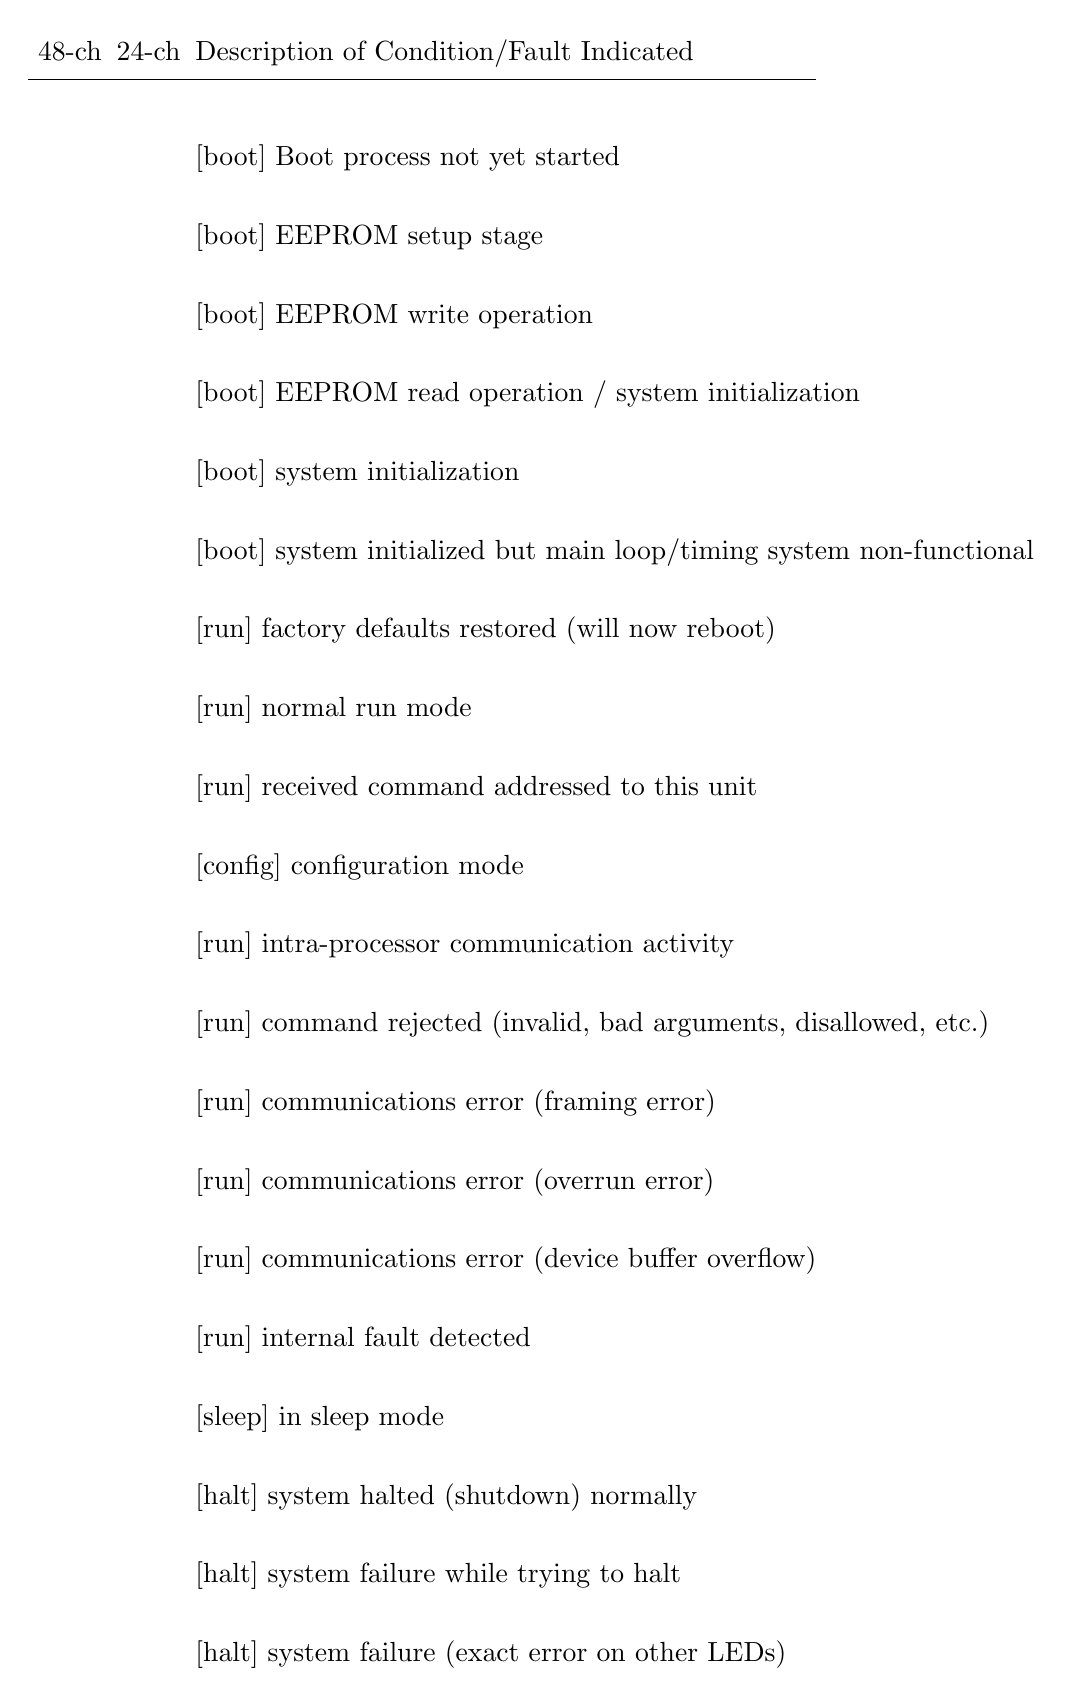
\begin{tikzpicture}
  \node [above right] at (2,11) {\strut Description of Condition/Fault Indicated};
  \node [above right] at (0,11) {\strut 48-ch};
  \node [above right] at (1,11) {\strut 24-ch};
  \draw (0,11) -- (10,11);
  \def\y{10}
  \light{A}{off}\light{G}{off}\light{Y}{off}\light{R}{off}\light{G2}{off}\light{Y2}{off}\light{R2}{off}
  \node [right] at (2,\y) {[boot] Boot process not yet started};
  \def\y{9}
  \light{A}{off}\light{G}{off}\light{Y}{off}\light{R}{on}\light{G2}{off}\light{Y2}{off}\light{R2}{off}
  \node [right] at (2,\y) {[boot] \acronym{EEPROM} setup stage};
  \def\y{8}
  \light{A}{off}\light{G}{off}\light{Y}{on}\light{R}{on}\light{G2}{off}\light{Y2}{off}\light{R2}{off}
  \node [right] at (2,\y) {[boot] \acronym{EEPROM} write operation};
  \def\y{7}
  \light{A}{off}\light{G}{off}\light{Y}{on}\light{R}{off}\light{G2}{off}\light{Y2}{off}\light{R2}{off}
  \node [right] at (2,\y) {[boot] \acronym{EEPROM} read operation / system initialization};
  \def\y{6}
  \light{A}{off}\light{G}{on}\light{Y}{on}\light{R}{off}\light{G2}{off}\light{Y2}{off}\light{R2}{off}
  \node [right] at (2,\y) {[boot] system initialization};
  \def\y{5}
  \light{A}{off}\light{G}{on}\light{Y}{off}\light{R}{off}\light{G2}{off}\light{Y2}{off}\light{R2}{off}
  \node [right] at (2,\y) {[boot] system initialized but main loop/timing system non-functional};
  \def\y{4}
  \light{A}{ffl}\light{G}{ffl}\light{Y}{ffl}\light{R}{ffl}\light{G2}{ffl}\light{Y2}{ffl}\light{R2}{ffl}
  \node [right] at (2,\y) {[run] factory defaults restored (will now reboot)};
  \def\y{3}
  \light{A}{off}\light{G}{sfd}\light{Y}{off}\light{R}{off}\light{G2}{off}\light{Y2}{off}\light{R2}{off}
  \node [right] at (2,\y) {[run] normal run mode};
  \def\y{2}
  \light{A}{blk}\light{G}{sfd}\light{Y}{x}\light{R}{x}\light{G2}{x}\light{Y2}{x}\light{R2}{x}
  \node [right] at (2,\y) {[run] received command addressed to this unit};
  \def\y{1}
  \light{A}{off}\light{G}{ffl}\light{Y}{off}\light{R}{off}\light{G2}{off}\light{Y2}{off}\light{R2}{off}
  \node [right] at (2,\y) {[config] configuration mode};
  \def\y{0}
  \light{A}{x}\light{G}{x}\light{Y}{blk}\light{R}{x}\light{G2}{x}\light{Y2}{blk}\light{R2}{x}
  \node [right] at (2,\y) {[run] intra-processor communication activity};
  \def\y{-1}
  \light{A}{x}\light{G}{x}\light{Y}{x}\light{R}{on}\light{G2}{x}\light{Y2}{x}\light{R2}{x}
  \node [right] at (2,\y) {[run] command rejected (invalid, bad arguments, disallowed, etc.)};
  \def\y{-2}
  \light{A}{x}\light{G}{x}\light{Y}{on}\light{R}{ffl}\light{G2}{x}\light{Y2}{x}\light{R2}{x}
  \node [right] at (2,\y) {[run] communications error (framing error)};
  \def\y{-3}
  \light{A}{x}\light{G}{x}\light{Y}{ffl}\light{R}{ffl}\light{G2}{x}\light{Y2}{x}\light{R2}{x}
  \node [right] at (2,\y) {[run] communications error (overrun error)};
  \def\y{-4}
  \light{A}{x}\light{G}{x}\light{Y}{sfd}\light{R}{ffl}\light{G2}{x}\light{Y2}{x}\light{R2}{x}
  \node [right] at (2,\y) {[run] communications error (device buffer overflow)};
  \def\y{-5}
  \light{A}{ffl}\light{G}{sfd}\light{Y}{ffl}\light{R}{off}\light{G2}{x}\light{Y2}{x}\light{R2}{x}
  \node [right] at (2,\y) {[run] internal fault detected};
  \def\y{-6}
  \light{A}{off}\light{G}{sfl}\light{Y}{sfl}\light{R}{sfl}\light{G2}{sfl}\light{Y2}{sfl}\light{R2}{sfl}
  \node [right] at (2,\y) {[sleep] in sleep mode};
  \def\y{-7}
  \light{A}{off}\light{G}{off}\light{Y}{off}\light{R}{sss}\light{G2}{off}\light{Y2}{off}\light{R2}{sss}
  \node [right] at (2,\y) {[halt] system halted (shutdown) normally};
  \def\y{-8}
  \light{A}{ffl}\light{G}{off}\light{Y}{ffl}\light{R}{ffl}\light{G2}{off}\light{Y2}{off}\light{R2}{off}
  \node [right] at (2,\y) {[halt] system failure while trying to halt};
  \def\y{-9}
  \light{A}{x}\light{G}{x}\light{Y}{x}\light{R}{ffl}\light{G2}{x}\light{Y2}{x}\light{R2}{x}
  \node [right] at (2,\y) {[halt] system failure (exact error on other \acronym{LED}s)};
  
    
%  \def\ON#1#2#3{\CO{#1}{#2}{#3} \draw (#1,#2) circle (.1);}
%  \def\CO#1#2#3{\draw [fill, color=#3] (#1,#2) circle (.1);}
%   \ON{.0}{.0}{yellow}\ON{.3}{.0}{green}\ON{.6}{.0}{yellow}\ON{.6}{.0}{red}
 \end{tikzpicture}
 \caption{Diagnostic \acronym{LED} Patterns\label{fig:leds}}
\end{figure}

\begin{figure}
 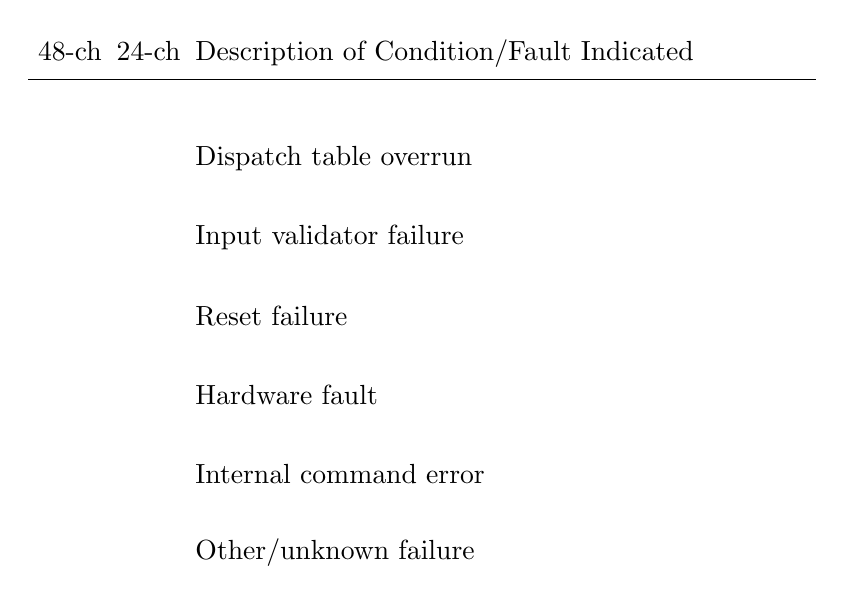
\begin{tikzpicture}
  \node [above right] at (2,10) {\strut Description of Condition/Fault Indicated};
  \node [above right] at (0,10) {\strut 48-ch};
  \node [above right] at (1,10) {\strut 24-ch};
  \draw (0,10) -- (10,10);
 \def\y{9}
  \light{A}{ffl}\light{G}{x}\light{Y}{ffl}\light{R}{off}\light{G2}{ffl}\light{Y2}{off}\light{R2}{off}
  \node [right] at (2,\y) {Dispatch table overrun};
 \def\y{8}
  \light{A}{ffl}\light{G}{x}\light{Y}{ffl}\light{R}{off}\light{G2}{x}\light{Y2}{off}\light{R2}{on}
  \node [right] at (2,\y) {Input validator failure};
 \def\y{7}
  \light{A}{ffl}\light{G}{x}\light{Y}{ffl}\light{R}{off}\light{G2}{ffl}\light{Y2}{ffl}\light{R2}{ffl}
  \node [right] at (2,\y) {Reset failure};
 \def\y{6}
  \light{A}{ffl}\light{G}{x}\light{Y}{ffl}\light{R}{off}\light{G2}{x}\light{Y2}{off}\light{R2}{ffl}
  \node [right] at (2,\y) {Hardware fault};
 \def\y{5}
  \light{A}{ffl}\light{G}{x}\light{Y}{ffl}\light{R}{off}\light{G2}{x}\light{Y2}{off}\light{R2}{sfd}
  \node [right] at (2,\y) {Internal command error};
 \def\y{4}
  \light{A}{ffl}\light{G}{x}\light{Y}{ffl}\light{R}{off}\light{G2}{off}\light{Y2}{ffl}\light{R2}{off}
  \node [right] at (2,\y) {Other/unknown failure};
 \end{tikzpicture}
 \caption{Internal Fault Condition Codes\label{fig:leds-errors}}
\end{figure}

\begin{figure}
 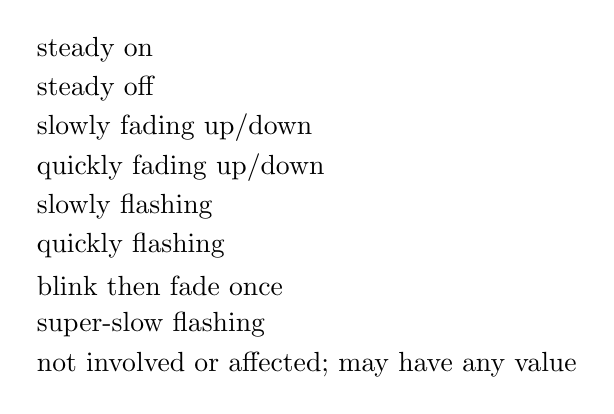
\begin{tikzpicture}
 \def\y{5}
  \light{Y2}{on} \node [right] at (1,\y) {steady on};
 \def\y{4.5}
  \light{Y2}{off} \node [right] at (1,\y) {steady off };
 \def\y{4}
  \light{Y2}{sfd} \node [right] at (1,\y) {slowly fading up/down};
 \def\y{3.5}
  \light{Y2}{ffd} \node [right] at (1,\y) {quickly fading up/down};
 \def\y{3}
  \light{Y2}{sfl} \node [right] at (1,\y) {slowly flashing};
 \def\y{2.5}
  \light{Y2}{ffl} \node [right] at (1,\y) {quickly flashing};
 \def\y{2}
  \light{Y2}{blk} \node [right] at (1,\y) {blink then fade once};
 \def\y{1.5}
  \light{Y2}{sss} \node [right] at (1,\y) {super-slow flashing};
 \def\y{1}
  \light{Y2}{x} \node [right] at (1,\y) {not involved or affected; may have any value};
 \end{tikzpicture}
 \caption{Key to LED Patterns\label{fig:leds-key}}
\end{figure}

\begin{figure}
 \begin{tabular}{rl}
  \z{0x01} & Command interpreter dispatch overrun \\
  \z{0x02} & Pass-down command in non-master \acronym{ROM} (set level)\\
  \z{0x03} & Pass-down command in non-master \acronym{ROM} (bulk update)\\
  \z{0x05} & Command interpreter dispatch overrun (in state 6)\\
  \z{0x06} & Pass-down command in non-master \acronym{ROM} (ramp level)\\
  \z{0x07} & Command interpreter dispatch overrun (in state 9)\\
  \z{0x08} & Command interpreter dispatch overrun (in state 10, non-slave)\\
  \z{0x0A} & Bad sentinel byte in internal command\\
  \z{0x0B} & Command interpreter dispatch overrun (internal commands)\\
  \z{0x0C} & Command interpreter dispatch overrun (internal commands)\\
  \z{0x0D} & Command interpreter dispatch overrun (state 13)\\
  \z{0x0E} & Command interpreter dispatch overrun (state 17)\\
  \z{0x0F} & Could not determine \acronym{ROM} type (query)\\
  \z{0x10} & Operation on wrong \acronym{ROM} type (query)\\
  \z{0x11} & Device does not support T/$\overline{\hbox{R}}$ operation \\
  \z{0x12} & Code executed on wrong \acronym{ROM} (M/S communication) \\
  \z{0x20} & Invalid command\\
  \z{0x21} & Configuration-mode command outside configuration mode\\
  \z{0x22} & Command not implemented\\
  \z{0x23} & Command incomplete\\
  \z{0x70} & Failed to reset following factory default restore\\
 \end{tabular}
 \caption{Error Condition Codes Reported Via Query Command\label{fig:errcodes}}
\end{figure}



%\section{Numeric Error Codes}
\chapter{Lumos CLI Command Manual Entries}\label{ch:lumosctl}
This chapter provides the documentation for the \z{lumosasm}, \z{lumosctl}, and \z{lumosupgrade} commands.  
This same information is also
provided to the \acronym{CLI} user on Unix, Linux, or Macintosh systems via the \z{man} command.  

In this documentation, the following typographical conventions are used:
\begin{itemize}
	\item	\Var*{Variables}, which indicate values to be replaced with suitable values when you
		invoke the program, are shown in Italic type inside angle brackets.  (The angle brackets
		are not typed as part of the command syntax.)
	\item	\z{Literal text} which should be typed as-is, as well as the names of commands, is set
		in fixed-width text.
	\item	\emph{File names} are set in Italics.  Italics are also used for general points of emphasis.
	\item	{}[Optional values] are enclosed in square brackets.  These may be omitted if appropriate.
		(The brackets themselves are not typed as part of the command syntax.)
\end{itemize}
References to other program manual entries look like ``\z{lumosctl}(1)'' which indicates that the
\z{lumosctl} command is documented in section~1 of the manual, which is the section for general 
user commands on Unix-like systems.
\newpage
\index{lumosasm@\z{lumosasm}}
\begin{NotImplemented*}{The \z{lumosasm} program is used to assemble descriptions of stored
sequences into the internal binary format recognized by the Lumos boards.  Since that feature is
not yet supported by Lumos boards, this section of the manual is blank until that feature is
fully defined.}
%\input lumosasm
\end{NotImplemented*}
\newpage
\index{lumosctl@\z{lumosctl}}
\input lumosctl
\newpage
\index{lumosupgrade@\z{lumosupgrade}}
\label{man:lumosupgrade}
\input lumosupgrade
\chapter{Troubleshooting}
While we anticipate the Lumos board will provide many hours of worry-free operation,
as with any device (particularly one built as a \acronym{DIY} project), sometimes things don't go
quite as planned.  Here are a few common problems and their solutions.

\begin{longtable}{|p{1.5in}|p{1.5in}|p{2in}|}\hline
\bfseries Symptom & \bfseries Likely Cause(s) & \bfseries Solution \\\hline\hline
\endhead
An entire block of outputs does not turn on 
	& No power to the block 
	& If the \mc{BLOCK PWR} light is off, check the fuse for that block, 
	  the connection from the power supply to the block, and that the power supply is powered on.\\
\cline{2-3}
	& Power supply not told to wake up (\mc{ATX}-style supplies only).
	& Check that the power supply's green wire is attached to the $\overline{\hbox{\mc{PWR CTL}}}$
	  terminal on J9. \\
\cline{3-3}
	&& If the \acronym{LED}s on the board show that it is in sleep mode,  send it a ``wake'' command
	from the PC or just command it to turn on any output channel.
\\\hline
Some outputs don't work, or are erratic.
	& Loose % opto-isolator 
chip.
	& Lightly press chips U0--U5 back into their sockets.\\
\cline{2-3}
	& Bad solder connection or loose chip.
	& Re-check all solder connections on the board, re-solder any which are cold, broken, or
	  incomplete.\\\hline
No units in serial network respond to commands.
	& Missing terminator
	& Replace terminators on both ends of the daisy chain (note the PC's RS485 converter
	  may include a built-in terminator for that position).\\\hline
One unit does not respond to commands.
	& Wrong address.
	& Use the \verb+lumosctl+ program to reconfigure the board to have
	  the correct address.\\
\cline{2-3}
	& Blown communication fuse.
	& Replace fuse F3.\\\hline
\end{longtable}

If all else fails, try performing a factory reset as described in section \ref{ss:factoryreset} (page~\pageref{ss:factoryreset}).

\chapter{Glossary}\label{ch:glossary}
\begin{description}
	\item[Address:]
		The \mc{ID} number assigned to a particular device to uniquely distinguish it from the other
		devices plugged into the same serial connection.  The commands sent to Lumos boards all contain
		a ``target address'' which identifies the particular Lumos board which is to act on that command.
		All the other Lumos boards will ignore it.
	\item[Baud Rate:]
		The speed, in bits per second, of data that is transferred over a serial cable.  The term
		``baud'' refers to the number of electrical state changes per second made to perform the signalling.
		For the kind of signalling done by Lumos boards, the baud rate is the same as the bit-per-second rate,
		although for other applications such as high-speed modems, it would be more correct to refer to the
		bit-per-second (\acronym{BPS}) rate only.  Depending on the exact protocol settings used, one character
		takes approximately 10~bits to send, so a data rate of 9600~baud would send about 960 characters (bytes)
		per second.
	\item[Active Low:]
		A logic signal which is considered ``on'' when the signal is ``low'' (binary 0 or 0\,V),
		and ``off'' when the signal is ``high'' (binary 1 or +5\,V).  Lumos relay circuits are 
		triggered with active-low signals.
	\item[\acronym{CLI}]
		Command-line interface.  A program launched on the command-line, or ``shell,'' interface of the computer---the
		\z{cmd} window on Microsoft Windows, or the shell in a Mac \acronym{OSX} or Unix/Linux terminal window or
		\z{xterm}.  Typically \acronym{CLI} tools interact with the user via keyboard, often using a combination of
		``options'' or ``switches'' to control the program's behavior rather than using a mouse or other graphical
		interfaces.  Generally, \acronym{CLI} tools are easier to automate (to have the computer run them autonomously
		on a schedule or as needed) since most of them are designed to be run unattended, specifying all of the parameters needed right on the command line.
	\item[\acronym{DIY}:] ``Do-It-Yourself.''
	\item[Duplex:]
		a feature of a serial line.  On a full-duplex connection, separate data wires are present
		to carry data in both directions, so one device can send and receive data at the same time.
		On a half-duplex connection, only a single set of data wires is present, so devices must
		take turns transmitting over them.
	\item[Factory reset:]
		The process of resetting all user-configurable options on a device to their original state, as the
		device presumably was shipped ``in the box'' from its factory.  Lumos boards can be reset in this manner
		as described on page~\pageref{ss:factoryreset}.
	\item[Jumper Block:]
		A series of pins mounted to the \acronym{PCB}.  Different options are configured for the
		circuit by placing a \ix{jumper} over certain pairs of pins, shorting them together.
	\item[\acronym{LED} (Light Emitting Diode):]
		A special kind of diode which emits light when current passes from its anode to its cathode.
	\item[\acronym{MOSFET}:]
		The type of transistor which forms the major part of a Lumos DC relay channel.  The name
		is an acronym for Metal Oxide Semiconductor Field Effect Transistor.
	\item[\acronym{PCB} (Printed Circuit Board):]
		The board where electronic components are mounted to form a complete circuit.  Metal
		traces are ``printed'' (actually etched) onto the surface of the board itself to make the
		connections between components.
	\item[Power Cycle:]
		To turn the power off, then on, thus resetting the state of the device.  On a Lumos board,
		the same effect can be had by pressing the \acronym{RESET} button momentarily, although
		power cycling works, too.  Note that this does not undo any permanent settings such as device
		address or baud rate.  To return all settings to their original values, you must perform a
		full factory reset.
	\item[RS-232:]
		A standard hardware protocol for sending serial data between two devices (such as a computer
		and a modem or a single Lumos board).  Shielded cable should be used for best results, and
		the cable length should not exceed 25\,ft.
	\item[RS-485:]
		A standard hardware protocol for sending serial data between multiple devices on a single
		cable length (electrically it is a single cable which each device ``taps into'' along the
		line; physically it is typically a ``daisy chain'' arrangement where a short cable connects
		one device to the next, another cable to the next, and so on). Unshielded twisted-pair cable
		is used (like Ethernet cable), and the cable lengths should not exceed a total of 4,000\,ft
		(1,200\,m).
	\item[\acronym{SSR} (Solid-State Relay):] A device which controls an external power load.  In
		contrast to a mechanical relay, an \acronym{SSR} has no moving parts, but does its switching
		electronically.
	\item[Terminator Plug:]
		An RS-485 network requires a terminator at each end.  This is a small plug which plugs into
		the last unit in the daisy chain.
	\item[\acronym{TTL} (Transistor-Transistor Logic):] One of the ways digital logic circuits can be
		constructed.  For our purposes here, we consider a ``\acronym{TTL}-level'' signal to be a
		logic input or output where a voltage near +5\,V is ``high'' (binary 1 or ``true'') and a
		voltage near 0\,V is ``low'' (binary 0 or ``false'').  The inputs should never be above
		+5 nor below 0 volts.
\end{description}

\input acknowledgements

\indexintoc
\printindex
\clearpage

\input colophon

\end{document}
